\documentclass[12pt]{report}

% ---------------- PACKAGES ----------------
\usepackage[spanish]{babel}
\usepackage{csquotes}
\usepackage[T1]{fontenc}
\usepackage{setspace}
\usepackage[
top=0.5cm,
bottom=2.5cm,
left=3cm,
right=2.5cm
]{geometry}
\usepackage{graphicx}
\usepackage[colorlinks=true, linkcolor=black]{hyperref}
\usepackage{longtable}
\usepackage{parskip} % Elimina la sangría y añade un espaciado automático y limpio entre párrafos
\setlength{\parindent}{0pt} % Asegura que la sangría sea cero en todo el documento si prefieres el estilo de bloque
\usepackage{siunitx}
\usepackage{ragged2e}
\usepackage{amsmath}
\usepackage{comment}
\usepackage{ragged2e}   % Para alineaciones fluidas sin guionizado extraño (\RaggedRight)
\usepackage{verbatim} %Permite hacer comentario de varios bloques de texto
\usepackage{booktabs} %Ayuda a hacer tablas bonitas
\usepackage{array} % Ayuda a las tablas bonitas
\usepackage{tabularx}
\usepackage{tikz} %Diagramas
\usetikzlibrary{shapes.geometric, arrows, positioning}
\usepackage{float}
\usepackage{xcolor}
\usetikzlibrary{calc}
\usepackage{multirow}
\usepackage{pifont}
\usepackage{amssymb}
\usepackage{adjustbox}
\usepackage{enumitem}
\usepackage{subcaption}

\newcolumntype{Y}{>{\raggedright\arraybackslash}X} %Es para las tablas, para evitar el error de overfull hbox, y que el texto se ajuste a la celda de la tabla

\addto\captionsspanish{
  \renewcommand{\contentsname}{Contenido}
}
% Definición de estilos para el diagrama
\tikzset{
    block/.style={rectangle, draw, fill=white, text width=3cm, text centered, rounded corners, minimum height=1.2cm},
    cloud/.style={ellipse, draw, fill=gray!10, text width=2.5cm, text centered, minimum height=0.8cm},
    decision/.style={diamond, draw, fill=white, text width=2cm, text centered, aspect=2},
    detail/.style={rectangle, draw, fill=white, text width=3.5cm, font=\footnotesize, text centered, dashed},
    myarrow/.style={thick, ->, >=stealth}
}
% ---------------- PAGE SETUP ----------------
\setlength{\emergencystretch}{3em} %Margen de ajuste
\overfullrule=5pt

\usepackage[backend=biber, style=ieee]{biblatex}
\addbibresource{Referencias.bib}
\usepackage{hyperref} 
\hypersetup{
    colorlinks=true,
    linkcolor=black,
    filecolor=magenta,      
    urlcolor=cyan,
    pdftitle={Tesis - Tu Nombre},
}


\usepackage{titlesec}

\titleformat{\chapter}[hang]
{\normalfont\Huge\bfseries}
{Capítulo \thechapter.}
{0.2em}
{}

\begin{document}

% ---------------- PAGE SETUP ----------------
\newgeometry{
  left=6.5cm,
  right=1.5cm,
  top=2.5cm,
  bottom=2.5cm
}
\thispagestyle{empty}
\begin{tikzpicture}[remember picture, overlay]

  % Línea vertical principal

  \node at (-3.3cm,-2cm)
    {
\includegraphics[width=4cm]{Escudo_Unison.png}};

    \node[align=center, font=\small]
  at (-3.3cm,-4.5cm)
  {“El saber de mis hijos \\
hará mi grandeza”
};

  \draw[line width=3pt,color=gray]
    (-2.9cm,-18cm) -- (-2.9cm,-5.5cm);


\draw[line width=3pt,color=gray]
    (-3.7cm,-18cm) -- (-3.7cm,-5.5cm);

    \node at (-3.3cm,-20.5cm)
    {
\includegraphics[width=4cm]{Logo-ITE.jpg}};
\end{tikzpicture}

% ---------------- DECORATIVE LINES ----------------


% ---------------- HEADER ----------------
\begin{center}
{\LARGE \textbf{UNIVERSIDAD DE SONORA}}\\[10pt]
{\color{gray}\rule{13cm}{3pt}}\\[6pt]
{\color{gray}\rule{13cm}{3pt}}\\[6pt]


{\large \textbf{DIVISIÓN DE CIENCIAS EXACTAS Y NATURALES}}\\[0.5cm]
\textbf{DEPARTAMENTO DE INVESTIGACIÓN EN FÍSICA}\\[0.5cm]
\textbf{Ingeniería en Tecnología Electrónica}
\end{center}

\vspace{2cm}

% ---------------- TITLE ----------------
\begin{center}
\textbf{“Diseño, modificación y evaluación de un sistema de manufactura aditiva tipo FDM con optimización del enfriamiento de capa y control térmico”}
\end{center}

\vspace{2cm}

% ---------------- AUTHOR ----------------
\begin{center}
\textbf{Tesis que presenta:}\\[8pt]
\textbf{JOSE ANGEL GONZALEZ MARTINEZ}
\\[8pt]
\end{center}

\vspace{1.8cm}

% ---------------- DEGREE ----------------
\begin{center}
Para obtener el título de\\[6pt]
\textbf{Ingeniero en Tecnología Electrónica}
\end{center}

\vspace{1.8cm}

% ---------------- DIRECTOR ----------------
\begin{center}
Director de tesis\\[6pt]
\textbf{Roberto Gomez Fuentes}
\end{center}

\vfill

% ---------------- FOOTER ----------------
\begin{center}
Hermosillo, Sonora \hfill mayo de 2026
\end{center}

% ---------------- LOGO ----------------

\vspace{0.5cm}




\newpage

\restoregeometry

\chapter*{Resumen}
\begin{comment}
Este proyecto se enfoca en diseñar y fabricar un sistema de fabricación aditiva tipo
FDM con enfoque académico. 

El control numérico computarizado ha estado en constante desarrollo en la industria manufacturera. Actualmente se ha popularizado en equipos FDM como
lo son las impresoras 3D, que han tenido adopción en el uso domestico. 
La industria manufacturera se centra en la automatización total y fabricación flexible, y estos equipos FDM han fomentado el crecimiento de esta 
tecnología en entornos educativos.

El objetivo es proporcionar a estudiantes una herramienta educativa, practica y asequible para poner en practica conocimientos adquiridos en el 
transcurso de su estadía en la licenciatura. Estos equipos FDM son totalmente modificables por el usuario, lo cual convierte a este proyecto en uno con alta
oportunidad de mejora constante respecto a equipos comerciales, que son sistemas mas cerrados. Este trabajo consta de objetivos
específicos como el diseño y armado, las piezas serán impresas con otro equipo FDM siguiendo la filosofía Reprap [1].
Se usó software libre "Marlin", el cual es un firmware dedicado a equipos de impresión 3D. Se realizó
calibración de los módulos que conforman el equipo, ajuste final y verificación del comportamiento. Asi también, se diseñó 
el sistema de enfriamiento del extrusor y fue comparado con uno comercial, tanto en eficiencia de enfriamiento y calidad de impresión final.
Se obtuvieron resultados superiores en ciertos aspectos a equipos comerciales, tanto en calidad como velocidad de impresión.
En conclusión, se logró un diseño que tiene mejoras con un equipo comercial, que tiene ventajas como ser completamente modificable y ser un sistema mas abierto,
lo que permite la integración en un entorno académico.
\end{comment}

Este proyecto presenta el diseño y fabricación de una impresora 3D basada en tecnología de Modelado por Deposición Fundida (FDM) orientada a aplicaciones académicas y de prototipado. El desarrollo del sistema se fundamentó en una arquitectura de hardware abierto inspirada en la filosofía RepRap, permitiendo la fabricación de múltiples componentes mediante manufactura aditiva y facilitando la modificación mecánica, electrónica y de firmware.

El diseño mecánico fue desarrollado mediante modelado CAD paramétrico en SolidWorks, mientras que el control electrónico se implementó utilizando una plataforma basada en Arduino Mega 2560, electrónica RAMPS 1.4 y firmware Marlin. Como parte del proyecto, se rediseñó el sistema de extrusión, logrando una reducción del 24.2\% en su masa, y se desarrolló un sistema de enfriamiento de capa que permitió reducir la temperatura del disipador del hotend en un 42.25\%. Posteriormente, se realizaron procesos de ensamblaje, calibración y ajuste experimental de parámetros de impresión, incluyendo la sintonización del controlador térmico PID del hotend. 

El desempeño del sistema se evaluó mediante pruebas de precisión dimensional 
(obteniendo errores inferiores al 0.3\%), pruebas de torre de temperatura para 
determinar la ventana térmica óptima (205~$^\circ$C), y el diagnóstico 
experimental de absorción de humedad en el filamento. Finalmente, se concluye 
que el sistema representa una plataforma funcional, modular y de bajo costo 
(\$4189 MXN), con alto potencial como herramienta didáctica para la enseñanza 
de manufactura aditiva, control numérico y sistemas embebidos.


\addcontentsline{toc}{chapter}{Resumen} 


\chapter*{Abstract}
\begin{comment}
This project focuses on the design and fabrication of an FDM (Fused Deposition Modeling) additive manufacturing system with an academic approach.

Computer numerical control (CNC) has undergone continuous development in the manufacturing industry and has recently become widespread in FDM equipment such as 3D printers, which have seen adoption in domestic environments. The manufacturing industry is increasingly focused on full automation and flexible manufacturing, and these FDM systems have contributed to the growth of this technology in educational settings.

The objective of this work is to provide students with an educational, practical, and affordable tool to apply the knowledge acquired throughout their undergraduate studies. These FDM systems are fully modifiable by the user, which makes this project one with a high potential for continuous improvement compared to commercial equipment, which typically consists of more closed systems. This work includes specific objectives such as the design and assembly of the system, with components manufactured using another FDM system following the RepRap philosophy [1].

Open-source software, specifically the Marlin firmware, was used for system control. Calibration of the system modules, final adjustments, and performance verification were carried out. Additionally, a custom extruder cooling system was designed and compared with a commercial counterpart in terms of cooling efficiency and final print quality.

The results obtained were superior in certain aspects compared to commercial equipment, particularly in print quality and printing speed. In conclusion, the developed system demonstrates improvements over commercial alternatives and offers advantages such as full modifiability and an open architecture, facilitating its integration into academic environments.
\end{comment}

This project presents the design and fabrication of a 3D printer based on 
Fused Deposition Modeling (FDM) technology oriented towards academic and 
prototyping applications. The system's development was based on an open-source 
hardware architecture inspired by the RepRap philosophy, allowing the 
manufacturing of multiple components through additive manufacturing and 
facilitating mechanical, electronic, and firmware modifications.

The mechanical design was developed using parametric CAD modeling in 
SolidWorks, while the electronic control was implemented using a platform 
based on an Arduino Mega 2560, RAMPS 1.4 electronics, and Marlin firmware. 
As part of the project, the extrusion system was redesigned, achieving a 
24.2\% reduction in its mass, and a layer cooling system was developed that 
reduced the hotend heatsink temperature by 42.25\%. Subsequently, assembly, 
calibration, and experimental tuning of printing parameters were carried out, 
including the tuning of the hotend's PID thermal controller.

System performance was evaluated through dimensional accuracy tests 
(obtaining errors below 0.3\%), temperature tower tests to determine the 
optimal thermal window (205~$^\circ$C), and the experimental diagnosis of 
moisture absorption in the filament. Finally, it is concluded that the system 
represents a functional, modular, and low-cost platform (\$4189 MXN) with 
high potential as an educational tool for teaching additive manufacturing, 
computer numerical control (CNC), and embedded systems.
\addcontentsline{toc}{chapter}{Abstract} 

\tableofcontents
\onehalfspacing

\listoffigures
\listoftables

\section*{Lista de Abreviaturas}
\addcontentsline{toc}{section}{Lista de Abreviaturas}

\begin{description}[font=\bfseries]
    \item[ABS:] Acrilonitrilo Butadieno Estireno
    \item[AM:] Additive Manufacturing (Manufactura Aditiva)
    \item[ASTM:] American Society for Testing and Materials
    \item[CAD:] Computer-Aided Design (Diseño Asistido por Computadora)
    \item[CNC:] Control Numérico Computarizado
    \item[FDM:] Fused Deposition Modeling (Modelado por Deposición Fundida)
    \item[G-Code:] Código de control numérico para impresoras 3D
    \item[GT2:] Tipo de correa dentada y polea
    \item[ISO:] International Organization for Standardization
    \item[NEMA:] National Electrical Manufacturers Association (estándar para motores paso a paso)
    \item[PETG:] Tereftalato de Polietileno Glicol
    \item[PID:] Proporcional-Integral-Derivativo
    \item[PLA:] Ácido Poliláctico
    \item[PTFE:] Politetrafluoroetileno (Teflón)
    \item[PWM:] Pulse Width Modulation (Modulación por Ancho de Pulso)
    \item[RAMPS:] RepRap Arduino Mega Pololu Shield (placa de control)
    \item[RepRap:] Replicating Rapid Prototyper (Proyecto de impresora 3D autorreplicable)
    \item[SLA:] Estereolitografía
    \item[SLS:] Sinterizado Selectivo por Láser
    \item[STL:] Standard Tessellation Language (Formato de archivo para impresión 3D)
\end{description}

\section*{Glosario}
\begin{itemize}
\item \textbf{Adhesión interlaminar}: Unión entre capas en una impresión 3D.
\item \textbf{Altura de capa}: Espesor de cada capa depositada en el proceso FDM.
\end{itemize}


\chapter{Introducción}
\begin{comment}
El proyecto presentado tiene como objetivo el diseño y fabricación de una impresora 3D de modelado por deposición fundida (FDM) optimizada para el uso de filamento PLA en entornos estudiantiles. El enfoque principal es proporcionar a los alumnos una plataforma de experimentación práctica y asequible que permita comprender a fondo la tecnología de Control Numérico por Computadora (CNC) y la manufactura aditiva.
 
Mediante el uso de herramientas de diseño asistido por computadora (CAD) como SolidWorks y plataformas de desarrollo de hardware abierto como Arduino, se ha desarrollado un sistema capaz de ser fabricado, en gran medida, por otra impresora 3D. Este concepto de "máquina autorreplicante" no solo reduce costos, sino que destaca la importancia del ensamblaje, la calibración y el ajuste mecánico como factores determinantes en la precisión final del equipo.

El desarrollo de esta impresora permite al estudiante involucrarse directamente en procesos de diseño, manufactura y calibración de sistemas de manufactura aditiva. Al enfrentarse al desafío de diseñar y fabricar la máquina desde sus componentes base, el estudiante desarrolla habilidades técnicas críticas y una capacidad de resolución de problemas que va más allá del uso de herramientas comerciales cerradas.
\end{comment}

La manufactura aditiva mediante Modelado por Deposición Fundida (FDM) representa hoy una de las tecnologías de mayor impacto en entornos educativos y de prototipado, debido a su bajo costo de implementación y a la flexibilidad que ofrece para la fabricación rápida de componentes funcionales. En particular, las impresoras 3D basadas en arquitecturas abiertas han permitido que estudiantes y desarrolladores puedan intervenir directamente en aspectos mecánicos, electrónicos y de control, favoreciendo el aprendizaje práctico de sistemas de manufactura automatizada.

El presente proyecto tiene como objetivo el diseño y fabricación de una impresora 3D tipo FDM orientada a aplicaciones académicas, utilizando filamento PLA como material principal de manufactura. El sistema fue desarrollado a partir de una arquitectura de hardware abierto inspirada en la filosofía RepRap. Para ello, 
se partió de la rehabilitación de un equipo institucional fuera de servicio, el cual no solo sirvió como referencia para identificar las limitaciones de las configuraciones comerciales, sino que se utilizó como herramienta de apoyo para fabricar los múltiples componentes estructurales de la nueva impresora, facilitando así futuras modificaciones mecánicas y electrónicas.

Para el desarrollo del equipo se emplearon herramientas de diseño asistido por computadora (CAD), específicamente SolidWorks, así como plataformas de control electrónico basadas en Arduino y firmware Marlin. Adicionalmente, se realizó un rediseño del módulo de extrusión y del sistema de enfriamiento de capa con el propósito de mejorar la estabilidad térmica y la calidad superficial de las piezas.Este desarrollo respondió a criterios de adaptación al contexto académico, incluyendo consideraciones de costo, disponibilidad de materiales y mejora del comportamiento térmico.

El desarrollo de esta plataforma permite al estudiante involucrarse directamente en el ciclo completo de un sistema de manufactura aditiva: desde el diseño mecánico y la integración electrónica hasta la calibración, el diagnóstico de fallas (como la absorción de humedad en el filamento) y el control numérico. De esta manera, el proyecto no solo representa una alternativa de bajo costo frente a equipos comerciales cerrados, sino también una herramienta didáctica capaz de fortalecer competencias técnicas relacionadas con sistemas embebidos, automatización y manufactura digital.

Finalmente, el presente documento se organiza de la siguiente manera: en el Capítulo 2 se expone el planteamiento del problema; en el Capítulo 3 se 
presentan los antecedentes y la justificación del proyecto; en el Capítulo 4 se definen los objetivos generales, específicos y las metas planteadas. 
Posteriormente, el Capítulo 5 desarrolla el marco teórico. En el Capítulo 6 se describe la metodología, que incluye la rehabilitación del equipo, el diseño del módulo de extrusión y los procesos de calibración. El Capítulo 7 presenta los resultados obtenidos y el Capítulo 8 expone la discusión de dichos resultados, contrastándolos con la literatura y reconociendo las 
limitaciones del trabajo. Finalmente, el Capítulo 9 presenta las conclusiones del proyecto, y el Capítulo 10 incluye las referencias bibliográficas que sustentan la investigación.



\chapter{Planteamiento del problema}
 En los últimos años, la impresión 3D ha pasado de ser una tecnología exclusiva de laboratorios especializados a convertirse en una herramienta presente en entornos industriales, educativos y domésticos. Esta popularidad ha generado una amplia oferta de arquitecturas comerciales orientadas al consumo general.

Sin embargo, gran parte de las impresoras 3D comerciales disponibles actualmente están orientadas a usuarios no especializados y priorizan una operación inmediata con mínima intervención técnica. Como consecuencia, muchos de estos equipos utilizan arquitecturas cerradas, firmware restringido y componentes propietarios que limitan las posibilidades de modificación y reparación del sistema por parte del usuario.

En entornos académicos y de investigación, esta dependencia tecnológica genera diversas problemáticas. La necesidad de utilizar refacciones específicas del fabricante incrementa los costos de mantenimiento y dificulta la reparación del equipo ante fallas menores. De igual manera, los tiempos asociados a procesos administrativos de adquisición pueden provocar largos periodos de inactividad en laboratorios universitarios. Desde el punto de vista formativo, el uso de sistemas cerrados limita la capacidad del estudiante para comprender e intervenir directamente en aspectos mecánicos, electrónicos y de control relacionados con la manufactura aditiva.

Frente a esta problemática, las plataformas basadas en hardware y software de código abierto representan una alternativa viable para el desarrollo de sistemas modificables, reparables y de bajo costo. La posibilidad de fabricar componentes propios y adaptar tanto el firmware como la arquitectura mecánica permite extender la vida útil del equipo y fortalecer el aprendizaje práctico en áreas relacionadas con control numérico computarizado (CNC), electrónica y diseño mecánico. Esta alternativa es especialmente pertinente en instituciones con recursos limitados, pues permite al estudiante interactuar con cada subsistema del equipo, diagnosticar fallas y proponer mejoras documentadas.

Por lo tanto, surge la necesidad de desarrollar una impresora 3D tipo FDM con arquitectura abierta y fácilmente mantenible, orientada a aplicaciones académicas, capaz de servir como plataforma didáctica para la experimentación y el aprendizaje práctico. Abordar esta necesidad es la parte central del presente proyecto, que busca no solo la construcción de un equipo funcional, sino también la creación de un entorno didáctico que permita a los estudiantes adquirir competencias en diseño, manufactura y control de sistemas de manufactura aditiva.


\begin{comment}
La impresión 3D, en todas sus presentaciones, emergió como una de las 
tecnologías mas emocionantes en la actualidad, mejorando el alcance de la 
fabricación y creación de objetos de manera automatizada. Con origen en 
laboratorios de investigación, llegó a convertirse en una 
herramienta omnipresente en industria e incluso en talleres y hogares de 
aficionados a la fabricación de todo el mundo. Debido a su aumento de 
popularidad, su oferta en el mercado aumentó, por lo cual vemos 
arquitecturas comerciales al alcance de cualquiera, conformándose como un
producto no solo para un sector sino que se proyecta como una maquina que
puede llegar a ser común en los hogares.

¿Cual es el problema?
El hecho de que estas maquinas están destinadas a usuarios un tanto mas 
casuales, como lo seria un investigador en un laboratorio o a personal 
de una fabrica, provoca que estos dispositivos sean mas cerrados al 
usuario; poco personalizables; usando tanto hardware y software de su 
propiedad.
\end{comment}
\begin{comment}
    La impresión 3D se ha consolidado como una de las tecnologías de mayor crecimiento en entornos industriales, educativos y de prototipado rápido. Lo que comenzó en laboratorios de investigación especializados se ha transformado en una herramienta omnipresente en la industria, talleres y hogares de aficionados. Esta popularidad ha generado una amplia oferta de arquitecturas comerciales que se proyectan como dispositivos comunes para el consumo masivo.

Sin embargo, esta masificación ha traído consigo un problema de diseño: la mayoría de estos equipos están destinados a un usuario no especializado que busca una experiencia de operación inmediata con mínima intervención técnica. Esto provoca que los dispositivos sean sistemas cerrados, poco personalizables y basados en hardware y software propietario.

Para una institución educativa o un laboratorio de investigación, este modelo de "caja negra" acarrea dificultades operativas graves:

Dependencia de repuestos oficiales: Cualquier avería obliga a la compra de componentes costosos y específicos del fabricante.

Dependencia administrativa: En el contexto de una universidad, depender de garantías oficiales o procesos de compra lentos a menudo condena a los equipos al desuso ante fallas menores.

Limitación del aprendizaje: Al no poder modificar el firmware o intervenir el hardware, el estudiante se limita a ser un operador de la máquina, perdiendo la oportunidad de entender la ingeniería detrás del proceso.

La transición hacia un equipo basado en tecnología de código abierto (Open Source) permite que las reparaciones y mejoras sean constantes, de bajo costo y accesibles mediante la modificación del firmware y la fabricación de piezas propias.

Por lo tanto, surge la necesidad de desarrollar una plataforma de impresión 3D abierta, modular y reparable que permita tanto el aprendizaje técnico como la reducción de costos operativos en entornos académicos.
\end{comment}


\chapter{Antecedentes y justificación}
\begin{comment}
Las maquinas comúnmente llamadas CNC no son más que un tipo de control utilizado para que una herramienta haga las operaciones que se le ordenen, puede ser adaptada a una gran variedad de herramientas, viene de las siglas en ingles “Computarized Numerical Control” o “Control Numérico Computarizado”.



Hacia los años 60 se podría decir que nace el control numérico computarizado gracias al avance y miniaturización de los componentes que utilizaba. Se pueden hablar de tres generaciones de control numérico de acuerdo con el avance que fue teniendo la electrónica: Válvulas electrónicas y relees (1950), Transistores (1960), Circuitos integrados (1965), Microprocesadores (1975) y actualmente se puede hacer con cualquier computadora ya sea de sobremesa o portátil. Ya que esta tan avanzado y estandarizado su uso que existe mucho software, incluso software libre para poder hacer una de estas máquinas casera. 

Las tendencias actuales en la industria manufacturera se centran en la automatización total y la fabricación flexible, utilizando máquinas CNC conectadas a un ordenador central para la programación y ejecución de tareas. El objetivo es eliminar la intervención humana en los procesos de producción, lo que mejora la eficiencia, calidad y reduce costos.
Al ser actualmente una forma de control muy utilizado en la industria manufacturera existen variados artículos que tocan este tema en particular. Un pequeño repaso a algunos artículos encontrados nos sirve para identificar que podemos hacer para mejorar la máquina que se quiere fabricar.

\end{comment}
\begin{comment}
Aunque la impresión 3D parece una tecnología reciente, sus bases se establecieron en la década de 1980. En 1984, Chuck Hull inventó la estereolitografía (SLA), fundando posteriormente 3D Systems. Años después, en 1989, se patentó el modelado por deposición fundida (FDM), tecnología que hoy domina el mercado de bajo costo. Durante décadas, estas ventajas estuvieron reservadas exclusivamente a la gran industria debido a costos que superaban los 30,000 dólares por equipo.

Esta exclusividad terminó en febrero de 2004, cuando Adrian Bowyer publicó el proyecto RepRap en la Universidad de Bath. La esencia de RepRap es la creación de una máquina de bajo costo capaz de replicarse a sí misma bajo la licencia GNU (General Public License). Este movimiento permitió que la tecnología se distribuyera globalmente, derivando en diseños emblemáticos como la Prusa i3, creada por Josef Prusa en 2012.

El presente proyecto se justifica en la necesidad de evolucionar estos diseños abiertos. Tomando como base la arquitectura de la Prusa i3, se ha implementado un rediseño del módulo de extrusión y el sistema de enfriamiento. Esta modificación busca no solo mantener la filosofía de bajo costo y reparabilidad del proyecto RepRap, sino también optimizar la calidad de impresión y la estabilidad térmica, adaptando el equipo a las exigencias del entorno académico actual.
\end{comment}



A pesar de su reciente popularización, las bases de la impresión 3D se establecieron durante la década de 1980 \cite{gibson2021,salazar2024}. En 1984, Chuck Hull desarrolló la estereolitografía (SLA), fundando posteriormente la empresa 3D Systems \cite{gibson2021}. Años más tarde, en 1989, se patentó el modelado por deposición fundida (FDM), tecnología que actualmente constituye una de las principales arquitecturas de impresión 3D de escritorio de bajo costo \cite{salazar2024}. Durante varios años, estas tecnologías permanecieron restringidas principalmente al sector industrial debido al elevado costo de los equipos y materiales especializados.

Esta limitación comenzó a reducirse en febrero de 2004, cuando Adrian Bowyer presentó el proyecto RepRap en la Universidad de Bath \cite{bowyer2004reprap}. La esencia de este proyecto consiste en desarrollar una impresora 3D de bajo costo capaz de fabricar parte de sus propios componentes, distribuyendo sus diseños y firmware bajo licencias abiertas. Este movimiento impulsó la expansión global de la manufactura aditiva de código abierto, dando origen a arquitecturas ampliamente adoptadas como la Prusa i3, desarrollada por Josef Prusa en 2012 \cite{prusa2012}.

Este recorrido histórico es relevante para el presente proyecto porque evidencia que la accesibilidad de la manufactura aditiva ha dependido históricamente de la apertura de sus diseños y de la capacidad de los usuarios para modificar y mejorar los sistemas existentes. Bajo esa misma filosofía, el presente trabajo toma como base la configuración mecánica cartesiana de la Prusa i3 y la adapta a las condiciones y criterios específicos del contexto académico en que fue desarrollado, incluyendo el rediseño del módulo de extrusión y del sistema de enfriamiento de capa.

En la actualidad, el ecosistema de hardware abierto derivado del proyecto RepRap continúa evolucionando. Arquitecturas como la Prusa MK4 han incorporado sistemas de extrusión directa, sensores de nivelación automática y marcos de aluminio extruido como respuesta a las limitaciones dinámicas y térmicas identificadas en generaciones anteriores \cite{prusaMK4}. Paralelamente, impresoras comerciales de gama media como la Bambu Lab A1 \cite{bambu_a1} o la Creality Ender 3 V3 \cite{creality_ender3v3} han popularizado sistemas de enfriamiento de capa con ventilación radial de múltiples salidas, mejorando la calidad en voladizos y puentes. Sin embargo, estos equipos mantienen arquitecturas parcial o totalmente cerradas, limitando su aplicabilidad como plataformas de experimentación académica. El presente proyecto se inserta en esta tendencia de evolución abierta, adoptando soluciones de diseño similares y adaptándolas a las condiciones y recursos de un entorno universitario.

Esta adaptación mantiene la filosofía de bajo costo, modularidad y reparabilidad propuesta por el proyecto RepRap, además de optimizar el desempeño del sistema y fortalecer su aplicación como herramienta didáctica para el aprendizaje de manufactura aditiva, control numérico computarizado y diseño mecánico.




\chapter{Objetivos y metas}
\section{Objetivo general}
Diseñar y fabricar una impresora 3D basada en tecnología FDM orientada a aplicaciones académicas, mediante el rediseño del sistema de extrusión y enfriamiento de capa, con el propósito de mejorar la calidad de impresión y evaluar su desempeño frente a equipos comerciales equivalentes.

\section{Objetivos específicos}
\begin{itemize}
  \item Diseñar la estructura mecánica y los componentes del sistema de impresión 3D mediante software CAD.
  \item Fabricar las piezas estructurales y funcionales utilizando procesos de manufactura aditiva.
  \item Integrar los sistemas mecánicos, electrónicos y térmicos de la impresora 3D.
  \item Configurar y calibrar el firmware de control para garantizar el correcto funcionamiento del equipo.
  \item Evaluar el comportamiento térmico del hotend y del sistema de enfriamiento de capa durante el proceso de impresión.
  \item Analizar la precisión dimensional y calidad superficial de las piezas fabricadas.
  \item Comparar el desempeño técnico y el costo del sistema desarrollado con impresoras comerciales de características similares.
  \item Validar la aplicabilidad del equipo como herramienta didáctica para entornos educativos y de prototipado.
\end{itemize}

\section{Metas}
Para dar cumplimiento a los objetivos planteados, se establecieron las 
siguientes metas concretas y medibles

\begin{enumerate}

\item Obtener una impresora 3D funcional basada en arquitectura abierta y tecnología FDM, lista para la impresión de piezas de prueba.

\item Lograr una reducción significativa en la masa del módulo de extrusión 
para disminuir la inercia sobre el carro del eje \(X\) y mejorar la dinámica 
del sistema.

\item Mejorar la disipación térmica del hotend y garantizar la integridad de 
los componentes del extrusor, evitando fallas por sobrecalentamiento o 
deformación.

\item Reducir la aparición de defectos de impresión como \textit{stringing}, \textit{warping} y \textit{ghosting} mediante la optimización de parámetros mecánicos y térmicos.

\item Obtener piezas con precisión dimensional y calidad superficial adecuadas para aplicaciones didácticas y de prototipado funcional.

\item Implementar un equipo con arquitectura abierta que permita futuras 
mejoras mecánicas, electrónicas y de firmware, así como la fácil sustitución 
de componentes.

\item Demostrar la viabilidad técnica y económica de la impresora, logrando 
un costo de fabricación inferior al de las alternativas comerciales 
equivalentes de gama baja.


\end{enumerate}





\chapter{Marco Teórico}
% =========================================================================
% 2.1 FUNDAMENTOS DE LA MANUFACTURA ADITIVA
% =========================================================================
\section{Fundamentos Básicos de la Tecnología FDM}
De acuerdo con la norma ISO/ASTM 52900:2021, la manufactura aditiva se define formalmente como la unión secuencial de materiales para fabricar objetos físicos tridimensionales a partir de datos digitales \cite{ISO52900}. A diferencia de los procesos sustractivos tradicionales, donde el material es removido de un bloque sólido mediante herramientas de corte, esta tecnología construye la geometría capa por capa. Aunque existen distintos métodos de manufactura aditiva, como la estereolitografía (SLA) y el sinterizado selectivo por láser (SLS), el Modelado por Deposición Fundida (FDM) es uno de los métodos más utilizados debido a su viabilidad económica, seguridad operacional, facilidad de mantenimiento y la amplia disponibilidad de plataformas de código abierto derivadas del proyecto RepRap \cite{jones2011reprap}, entre las cuales destaca la arquitectura Prusa i3 por su adopción global \cite{salazar2024}.

El proceso FDM utiliza filamento termoplástico continuo, el cual es introducido a un sistema de extrusión térmica denominado hotend. En este sistema, el material es calentado hasta alcanzar un estado semifundido y posteriormente depositado de manera controlada sobre una superficie de impresión siguiendo trayectorias definidas por código numérico (G-Code). Una vez depositado, el polímero se enfría y solidifica, formando capas sucesivas hasta completar la geometría deseada. Entre las principales ventajas de esta tecnología destacan la facilidad de fabricación de prototipos funcionales directamente desde modelos CAD, la accesibilidad económica de sus componentes y la amplia disponibilidad de materiales termoplásticos como PLA, ABS y PETG.

Sin embargo, el proceso presenta limitaciones inherentes a la fabricación por capas. La resistencia mecánica en el eje $Z$ suele ser inferior a la del plano horizontal ($X$-$Y$) debido a la unión interlaminar por difusión térmica parcial. Asimismo, la precisión dimensional y el acabado superficial pueden verse afectados por fenómenos de contracción térmica, vibraciones estructurales y variaciones en el flujo de extrusión.

Debido a estas limitaciones, el diseño del sistema de extrusión, la disipación térmica del hotend y el enfriamiento de capa representan factores críticos para mejorar la estabilidad del proceso y la calidad final de impresión en sistemas FDM de arquitectura abierta.

% =========================================================================
% 2.2 MATERIALES: EL ÁCIDO POLILÁCTICO
% =========================================================================
\section{Materiales: Ácido Poliláctico (PLA)}
% Esta sección es crítica para justificar el fallo térmico del primer intento.

El Ácido Poliláctico (PLA) es un poliéster termoplástico lineal derivado de la fermentación de fuentes de carbohidratos renovables, como el almidón de maíz o la caña de azúcar. En el ámbito de la manufactura aditiva por FDM, el PLA representa el material de mayor adopción debido a sus propiedades reológicas favorables, las cuales incluyen una baja tasa de contracción térmica y una excelente estabilidad dimensional durante el proceso de deposición. No obstante, sus propiedades térmicas intrínsecas imponen restricciones severas cuando se emplea en componentes estructurales expuestos a esfuerzos mecánicos y gradientes de temperatura moderados.



\subsection{Propiedades térmicas y mecánicas}
% Detallar los puntos de fusión y la temperatura de transición vítrea (Tg ~ 60°C).


A diferencia de los materiales cristalinos puramente definidos, los polímeros amorfos o semicristalinos como el PLA no poseen un punto de fusión térmico discreto, sino que exhiben transiciones de fase complejas en función de la temperatura \cite[Cap.~15]{callister2020}. Para el diseño de elementos mecánicos y estructurales, el parámetro termodinámico más crítico es la \textbf{Temperatura de Transición Vítrea ($T_g$)}.

\begin{itemize}
    \item \textbf{Temperatura de transición vítrea ($T_g$):} Para el PLA estándar, este valor se sitúa típicamente entre 55°C y 60°C \cite{chanda2006}. Al superar este umbral, el material pierde rigidez estructural y transita de un estado vítreo a un comportamiento viscoelástico, aumentando su susceptibilidad a deformaciones mecánicas.
    \item \textbf{Temperatura de Fusión ($T_m$):} Se localiza típicamente entre los \textbf{145°C y 160°C} \cite{chanda2006}. En esta región de transición de primer orden, los dominios cristalinos se desorganizan por completo, permitiendo que el polímero fluya con la viscosidad adecuada para ser forzado a través de una boquilla.
\end{itemize}

En lo que respecta a su comportamiento mecánico a temperatura ambiente, el PLA es un material rígido con buena estabilidad estructural y resistencia mecánica \cite{chanda2006}. Sin embargo, su principal desventaja es su fragilidad, ya que posee una baja capacidad de deformación antes de fracturarse (elongación a la rotura menor al 5\%)\cite{callister2020}. Físicamente, esto significa que ante un esfuerzo excesivo el material no se doblará de forma gradual, sino que se quebrará de manera repentina. Por esta razón, el diseño geométrico de las piezas de la impresora requirió consideraciones estructurales robustas, tales como esquinas redondeadas (filetes) y refuerzos en las zonas que soportan la mayor parte de las tensiones mecánicas para evitar rupturas prematuras.


\begin{comment}

La manufactura aditiva comprende un conjunto de tecnologías de fabricación capaces de producir objetos tridimensionales mediante la adición sucesiva de material a partir de información digital. A diferencia de los procesos de manufactura sustractiva, donde el material es removido de una pieza sólida mediante herramientas de corte, la manufactura aditiva construye la geometría capa por capa, permitiendo fabricar componentes complejos con menor desperdicio de material y mayor flexibilidad de diseño.

De acuerdo con la norma ISO/ASTM 52900:2021 \cite{ISO52900}, este proceso se define formalmente como la unión de materiales para fabricar objetos físicos tridimensionales a partir de datos digitales. Dentro de esta clasificación existen diversas tecnologías, tales como la estereolitografía (SLA), el sinterizado selectivo por láser (SLS) y el Modelado por Deposición Fundida (FDM), siendo esta última una de las más utilizadas debido a su bajo costo de implementación y facilidad de mantenimiento.



\subsection{Tecnología FDM}
El Modelado por Deposición Fundida (FDM, por sus siglas en inglés) utiliza materiales termoplásticos en forma de filamento continuo, los cuales son introducidos a un sistema de extrusión térmica denominado \textit{hotend}. En este sistema, el filamento es calentado hasta alcanzar un estado semifundido y posteriormente depositado de manera controlada sobre una superficie de impresión, siguiendo trayectorias definidas por código numérico (G-Code). Una vez depositado, el material se enfría y solidifica, formando capas sucesivas hasta completar la geometría deseada.

La tecnología FDM ha adquirido gran relevancia en entornos educativos y de prototipado rápido debido a la disponibilidad de plataformas abiertas como RepRap y Prusa i3, las cuales permiten al usuario modificar tanto la estructura mecánica como el firmware de control \cite{reprapWiki,prusaHistory}. Esta característica ha favorecido el desarrollo de sistemas de bajo costo orientados a la experimentación académica y al aprendizaje de tecnologías de control numérico computarizado.

% =========================================================================
% 5.1.1. FUNCIONAMIENTO DEL PROCESO FDM
% =========================================================================


\subsection{Funcionamiento del proceso FDM}
% Explicar el ciclo de extrusión, deposición y enfriamiento.
El funcionamiento de una impresora FDM puede dividirse en tres etapas fundamentales: alimentación del material, fusión térmica y solidificación controlada.
\begin{enumerate}
    \item\textbf{Alimentación del filamento:} Un motor de pasos acoplado a un sistema de engranajes ejerce una fuerza de empuje constante sobre el filamento termoplástico, guiándolo hacia la zona de calentamiento.
    \item \textbf{Fusión y extrusión:} El filamento atraviesa el \textit{hotend}, donde es calentado. El polímero alcanza un estado viscoelástico y es forzado a salir a través de una boquilla de diámetro reducido, generalmente de 0.4 mm.
    \item \textbf{Deposición y solidificación:} El material fundido es depositado sobre la superficie de impresión o sobre capas previamente solidificadas. Durante el enfriamiento ocurre la unión interlaminar entre filamentos adyacentes, fenómeno indispensable para garantizar la resistencia mecánica y estabilidad geométrica de la pieza final.
\end{enumerate}


\subsubsection{Ventajas y limitaciones tecnológicas}
% Breve análisis de costo/velocidad vs anisotropía (debilidad en eje Z).

La tecnología FDM presenta ventajas importantes en aplicaciones de prototipado y manufactura de bajo volumen; sin embargo, también posee limitaciones inherentes al proceso de deposición por capas.

\begin{description}
    \item[Ventajas:] Destaca principalmente por su accesibilidad económica y la facilidad de implementación. Permite fabricar prototipos funcionales directamente a partir de modelos CAD sin necesidad de herramientas especializadas o moldes de manufactura. Asimismo, la amplia disponibilidad de materiales termoplásticos como PLA, ABS, PETG y TPU permite adaptar las propiedades mecánicas y térmicas de las piezas a distintas aplicaciones.
    
    \item[Limitaciones:] La principal limitación del proceso es la anisotropía mecánirca generada por la fabricación capa por capa. Debido a que la unión entre filamentos depende de la difusión térmica parcial del polímero, la resistencia mecánica en el eje vertical ($Z$) suele ser inferior a la resistencia en el plano horizontal ($X-Y$). Además, la precisión dimensional puede verse afectada por fenómenos de contracción térmica, vibraciones estructurales y variaciones en el flujo de extrusión. Finalmente, el acabado superficial presenta una rugosidad escalonada característica (\textit{staircase effect}) determinada principalmente por la altura de capa seleccionada.
\end{description}

Debido a estas limitaciones, la estabilidad estructural, el control térmico y la correcta calibración de los parámetros de impresión representan factores críticos para mejorar la precisión dimensional y la repetibilidad en sistemas FDM de arquitectura abierta.

\end{comment}

%=========================================================================
% 5.3 ARQUITECTURA Y CINEMÁTICA DE IMPRESORAS FDM 
% ========================================================================
\section{Arquitectura Prusa i3 y Limitaciones Mecánicas}
La arquitectura mecánica de una impresora FDM determina la forma en que el sistema posiciona el cabezal de extrusión dentro del volumen de trabajo. En las impresoras de tipo cartesiano, el movimiento se realiza mediante tres ejes lineales ortogonales ($X$, $Y$ y $Z$), cada uno controlado de forma independiente mediante motores paso a paso y sistemas de guiado lineal \cite{groover2015}.

En la arquitectura Prusa i3, la distribución de componentes móviles se realiza de la siguiente manera: la cama calefactada se desplaza a lo largo del eje $Y$, el carro del extrusor se mueve a lo largo del eje $X$ sobre un puente vertical, y dicho puente se eleva en el eje $Z$ mediante dos husillos sincronizados que determinan la resolución de altura de capa.

Esta configuración introduce una limitación mecánica relevante: la cama es un elemento de masa considerable que cambia de dirección constantemente durante el proceso de impresión. Las fuerzas de inercia generadas producen vibraciones y momentos de flexión que se transmiten al marco estructural. Si la estructura carece de rigidez torsional suficiente, los microdesplazamientos resultantes se manifiestan en las piezas como ondulación superficial (\textit{ghosting}) y pérdida de precisión dimensional.

El diseño original de la Prusa i3 emplea un marco monolítico fabricado mediante corte de placa. No obstante, este tipo de estructura presenta limitaciones relacionadas con la dificultad de manufactura, menor modularidad y restricciones para implementar modificaciones mecánicas posteriores. 

Por esta razón, el diseño adoptado se baso en perfiles de aluminio tipo V-Slot de $20 \times 20$ mm, con el objetivo de incrementar la rigidez estructural, facilitar el ensamblaje modular y mejorar la estabilidad dinámica del sistema, así como la integración del módulo de extrusión rediseñado.




\begin{comment}
\section{Arquitectura y Cinemática de Impresoras FDM}

La fabricación de un objeto tridimensional en la tecnología FDM depende directamente de la capacidad del sistema mecánico para posicionar la boquilla de extrusión de forma precisa en un espacio tridimensional. La disposición de los actuadores, guías lineales y la estructura soporte determinan la estabilidad dinámica de la máquina durante el proceso de fabricación.

% =========================================================================
% 5.3.1 CINEMÁTICA CARTESIANA (TU SUBSECCIÓN)
% =========================================================================
\subsection{Cinemática Cartesiana y el modelo Prusa i3}

La mayoría de las impresoras 3D de escritorio de código abierto emplean un sistema de \textbf{cinemática cartesiana}. Este principio se fundamenta en la teoría de control numérico computarizado (CNC), donde la posición de cualquier punto en el espacio de trabajo se define mediante tres ejes lineales mutuamente perpendiculares entre sí ($X$, $Y$ y $Z$) \cite{groover2020}. Mecánicamente, esto implica que la máquina cuenta con actuadores independientes encargados de controlar el movimiento de forma dedicada en cada dirección dimensional.

Dentro de las configuraciones cartesianas, la arquitectura \textbf{Prusa i3} (perteneciente al proyecto RepRap) implementa un diseño específico donde los componentes móviles se dividen de la siguiente manera:

\begin{itemize}
    \item \textbf{Eje Y (Movimiento de la plataforma):} La superficie de impresión (cama calefactada) se desplaza longitudinalmente hacia adelante y hacia atrás sobre un par de guías lineales fijas a la base. En esta configuración, los motores deben desplazar constantemente el peso conjunto de la cama, el sistema de soporte y la pieza que se está fabricando.
    \item \textbf{Eje X (Movimiento del cabezal):} El carro del extrusor se desplaza de forma transversal de izquierda a derecha a lo largo de un eje montado sobre un puente vertical.
    \item \textbf{Eje Z (Movimiento vertical de elevación):} El puente completo que sostiene al eje X se desplaza de manera vertical mediante un sistema sincronizado de dos tornillos de avance (husillos) accionados por motores independientes. Este eje determina la resolución de la altura de capa.
\end{itemize}



Esta distribución de los componentes móviles introduce retos mecánicos críticos debido a las fuerzas de inercia generadas en el eje Y. Al ser la cama un elemento con un peso considerable que cambia de dirección constantemente a altas aceleraciones para depositar el material, se producen momentos de flexión y vibraciones que son transmitidos directamente hacia el marco vertical de la impresora.

Si el marco estructural original carece de la rigidez torsional suficiente, estas fuerzas provocan micro-desplazamientos y vibraciones en el puente del eje X. En la pieza final, esto se manifiesta visualmente como defectos geométricos de ondulación superficial (\textit{ghosting}) y una pérdida severa en la precisión dimensional. Por lo tanto, la sustitución del marco estructural por perfiles de aluminio V-Slot de alta rigidez estructural representa una solución de ingeniería orientada a mitigar las deficiencias dinámicas inherentes al constante movimiento del peso de la cama en la arquitectura Prusa i3.


\section{Sistema de movimimiento CNC}
- - - - - - UNA BREVE DESCRIPCION DEL FUNCIONAMIENTO BASICO DEL CONTROL NUMERICO COMPUTARIZADO Y LOS MOTORES A PASOS JUNTO CON LA CALIBRACION 
NECESARIA DE LOS DRIVERS UTILIZAOS $($ UN ESQUMATICO Y LA FOMRULA NECESARIA PARA OBTENER EL VOLTAJE DE REFERENCIA$)$ - - - - - - 
\end{comment}
% =========================================================================
% 5.4 SISTEMAS TÉRMICOS 
% =========================================================================
\section{Sistemas de extrusión y transferencia térmica}

El control de los cambios de temperatura en una impresora FDM es un factor determinante para garantizar la continuidad de la extrusión y la precisión dimensional de la pieza fabricada. El sistema térmico del cabezal de impresión se divide en dos regiones con requerimientos opuestos que coexisten en un espacio muy reducido: la zona de fusión y la zona de transición.

\subsection{Anatomía y dinámica del Hotend}

El hotend es el conjunto mecánico encargado de transferir energía térmica al filamento para derretirlo. Sus componentes principales operan bajo la siguiente dinámica:

\begin{itemize}
    \item \textbf{\textit{Heater block} (Bloque calefactor):} Bloque de aluminio o cobre que aloja un cartucho de resistencia eléctrica controlado mediante un lazo cerrado PID a través del firmware de la impresora. Este componente concentra el calor necesario para alcanzar la temperatura de fusión ($T_m$) del material.
    \item \textbf{\textit{Nozzle} (Boquilla):} Elemento roscado al \textit{heater block} que restringe el flujo del plástico fundido para depositarlo con un diámetro específico.
    \item \textbf{\textit{Heatbreak} (Garganta térmica):} Es el componente estructural más crítico del sistema. Funciona como un aislante térmico que separa el \textit{heater block} (zona caliente) del disipador de calor del \textit{coldend} (zona fría) \cite{salazar2024}. Su objetivo es generar un corte térmico abrupto en una distancia de apenas unos milímetros, evitando que el calor se propague hacia arriba a través del filamento sólido.
\end{itemize}

Si el \textit{heatbreak} falla y no disipa el calor remanente, el filamento de PLA alcanza su temperatura de transición vítrea ($T_g$) antes de entrar al bloque de fusión. Esto provoca que el filamento se ablande prematuramente dentro de la zona de guía y se expanda por la fuerza de empuje mecánica. Este fenómeno, conocido comúnmente como taponamiento térmico (\textit{heat creep}), incrementa drásticamente la fricción interna y bloquea por completo la impresión.

La temperatura del bloque calefactor es regulada mediante un lazo cerrado de control PID implementado en el firmware Marlin, cuya sintonización se describe en detalle en la sección de metodología.

\subsubsection{Control PID}

El control de la temperatura en el bloque calefactor se realiza mediante un 
lazo cerrado de control Proporcional-Integral-Derivativo (PID). Este sistema 
utiliza la lectura de un termistor para calcular el error entre la temperatura 
deseada y la real, ajustando dinámicamente la potencia suministrada al 
cartucho calefactor para mantener la temperatura lo más estable posible. La 
correcta sintonización de las constantes PID evita fluctuaciones térmicas que 
podrían afectar la viscosidad del polímero y la calidad de la extrusión. 
Marlin, el firmware utilizado, incorpora una función de autotuning que permite 
calcular estos valores de manera automática, como se detallará en la 
metodología.


\subsection{Ventilador de capa y enfriamiento del polímero}

Inmediatamente después de que el material fundido sale por el \textit{nozzle}, requiere un proceso de enfriamiento rápido dirigido por el \textbf{ventilador de capa}. Dado que el PLA retiene el calor de forma prolongada, es indispensable un flujo de aire forzado constante enfocado justo por debajo de la punta de la boquilla. 

Este enfriamiento continuo es necesario para acelerar la solidificación de la capa recién depositada, permitiendo que conserve su forma frente a la gravedad, especialmente al fabricar secciones en el aire (\textit{overhangs}) o puentes estructurales. Un flujo de aire insuficiente mantiene el PLA en un estado pastoso, resultando en deformaciones por contracción térmica y pérdida de calidad superficial.


\begin{comment}
\subsection{Disipación térmica en actuadores (Motores NEMA 17)}

Las restricciones térmicas de la impresora no se limitan exclusivamente al bloque de extrusión. Los motores de pasos encargados de empujar el filamento (específicamente el motor NEMA 17 instalado en el \textit{coldend}) disipan calor durante su operación continua.


Bajo condiciones de trabajo normales, la superficie metálica de un motor NEMA 17 puede alcanzar temperaturas estables de entre \textbf{45°C y 55°C}. Si el soporte estructural que une este motor con el extrusor se fabrica en PLA sin un aislamiento o disipador térmico intermedio, el material base operará de forma crítica justo en los límites de su $T_g$ ($55^\circ\text{C}$). 

Bajo estas condiciones, el esfuerzo y la tensión constante ejercidos por los resortes del mecanismo de empuje provocarán que el soporte de PLA comience a doblarse y deformarse lentamente. Esta deformación altera la alineación del mecanismo de empuje, provocando pérdida de pasos, desgaste irregular del filamento y fallas en la alimentación del sistema.


\end{comment}

\begin{comment}
    
% =================================================================
% 2.4 FLUJO DE TRABAJO DIGITAL
%==================================================================
\section{Flujo de Trabajo Digital: Del Modelado al Control}

El paso de una idea geométrica a un elemento físico funcional requiere de una cadena de procesamiento de software orientada al control numérico computarizado. Este flujo de trabajo digital actúa como el puente traductor entre el diseño abstracto en tres dimensiones y las señales eléctricas que los controladores envían a los actuadores mecánicos de la impresora FDM.


\begin{figure}[H]
\centering

\begin{tikzpicture}[
    node distance=1.5cm,
    block/.style={
        rectangle,
        draw=black,
        rounded corners,
        minimum width=6.5cm,
        minimum height=1.1cm,
        align=center
    }
]

\node (cad) [block] {
\textbf{Modelado CAD}\\
SolidWorks (.SLDPRT / .SLDASM)
};

\node (stl) [block, below=of cad] {
\textbf{Exportación de geometría}\\
Malla de triángulos (.STL / .3MF)
};

\node (cura) [block, below=of stl] {
\textbf{Laminado (\textit{Slicing})}\\
Software Ultimaker Cura
};

\node (gcode) [block, below=of cura] {
\textbf{Generación de trayectorias}\\
Código numérico (G-Code)
};

\node (marlin) [block, below=of gcode] {
\textbf{Control electrónico}\\
Firmware Marlin
};

\node (motion) [block, below=of marlin] {
\textbf{Movimiento y manufactura}\\
Deposición física de material
};

% Aquí usamos 'myarrow' que es tu estilo global
\draw [myarrow] (cad) -- (stl);
\draw [myarrow] (stl) -- (cura);
\draw [myarrow] (cura) -- (gcode);
\draw [myarrow] (gcode) -- (marlin);
\draw [myarrow] (marlin) -- (motion);

\end{tikzpicture}

\caption{Flujo de trabajo digital en impresión FDM.}
\label{fig:flujo_digital}
\end{figure}


Como se ilustra en la Figura \ref{fig:flujo_digital}, el proceso se compone de las siguientes etapas consecutivas:

\begin{enumerate}
    \item \textbf{Modelado Geométrico (CAD):} Consiste en la generación matemática de los volúmenes en un entorno de diseño asistido por computadora. Para las modificaciones estructurales de este proyecto, esta etapa permitió simular el acoplamiento mecánico entre los perfiles de aluminio y las nuevas piezas del extrusor antes de su manufactura.
    \item \textbf{Discretización de la Malla (STL):} La geometría continua del CAD se exporta a un formato de malla poligonal, típicamente STL (\textit{Stereolithography}). Este formato aproxima la superficie externa del modelo mediante una red tridimensional de triángulos interconectados, perdiendo la información de operaciones paramétricas pero conservando la fidelidad de la forma exterior.
    \item \textbf{Procesamiento de Laminado (\textit{Slicing}):} El archivo de malla es procesado por un software laminador (en este caso, Ultimaker Cura). El programa rebana virtualmente el objeto en capas horizontales de altura constante y calcula los parámetros de manufactura esenciales: velocidad de desplazamiento, porcentaje de relleno (\textit{infill}), estructuras de soporte y multiplicadores de extrusión.
    \item \textbf{Generación de G-Code:} Como resultado del laminado, el software exporta un archivo de texto plano con instrucciones en código estándar ISO G-Code. Este archivo contiene comandos secuenciales de coordenadas lineales ($G1 \, X_x \, Y_y \, Z_z \, E_e$) que dictan la posición espacial del cabezal y el volumen exacto de filamento que debe ser extruido.
    \item \textbf{Interpretación del Firmware (Marlin):} El archivo G-Code es transferido a la tarjeta de control de la impresora. El firmware (Marlin) actúa como el núcleo del sistema embebido; procesa el código línea por línea, ejecuta los algoritmos de aceleración y planeación de movimientos (\textit{look-ahead}), y traduce las coordenadas espaciales en trenes de pulsos coordinados para los controladores de los motores de pasos.
\end{enumerate}

Por esta razón, el control preciso del flujo digital desde el modelado CAD hasta la ejecución del firmware representa un elemento crítico para asegurar la precisión dimensional y la estabilidad mecánica del sistema desarrollado.

\end{comment}
\begin{comment}
    \subsection{Modelado paramétrico (CAD) y laminado (\textit{Slicing})}

La primera etapa del proceso consiste en diseñar la pieza en un software CAD paramétrico, como SolidWorks. A diferencia de un dibujo digital común, el modelado paramétrico permite definir las dimensiones de las piezas mediante relaciones matemáticas y restricciones mecánicas. Para este proyecto, esta herramienta fue indispensable para diseñar el nuevo sistema de extrusión, ya que permitió verificar de forma virtual que el eje del motor de pasos, el engranaje de empuje y la entrada del \textit{heatbreak} estuvieran perfectamente alineados antes de fabricar los componentes reales.

Una vez que el diseño del ensamble es correcto, la geometría se exporta al formato estándar STL. Este formato traduce las superficies sólidas del diseño en una malla compuesta por miles de triángulos interconectados. Como la tarjeta electrónica de la impresora no puede leer este archivo de tres dimensiones directamente, se requiere un software intermedio llamado laminador (o \textit{slicer}), utilizando para este trabajo el programa Ultimaker Cura \cite{gillespie2015}.

El laminador se encarga de rebanar el modelo 3D en capas horizontales delgadas según la altura de capa seleccionada. Al mismo tiempo, el software calcula las trayectorias de movimiento que debe seguir el cabezal, las velocidades de traslado y la cantidad exacta de plástico que se debe inyectar. Finalmente, toda esta información se traduce y se guarda en un archivo de texto plano con instrucciones secuenciales en formato G-Code, listo para ser ejecutado por la máquina.

\end{comment}




% =========================================================================
% 2.5 PARÁMETROS DE CALIDAD Y PRECISIÓN
% =========================================================================

\section{Calidad de Impresión y Precisión Dimensional}

La evaluación del desempeño de una impresora FDM no depende únicamente del funcionamiento mecánico de sus componentes, sino también de la calidad dimensional y superficial de las piezas fabricadas. Factores como la estabilidad estructural, el control térmico del hotend y el enfriamiento del material influyen directamente en la precisión geométrica obtenida durante el proceso de impresión.

En materiales termoplásticos como el PLA, la deposición y solidificación sucesiva del polímero generan fenómenos de contracción térmica que producen variaciones dimensionales respecto al modelo CAD original \cite{gibson2021}. Debido a ello, el diseño de componentes funcionales requiere considerar tolerancias mecánicas adecuadas, especialmente en piezas destinadas al montaje de elementos rígidos como rodamientos lineales, motores o sistemas de guiado.

Adicionalmente, las condiciones térmicas y dinámicas del sistema pueden provocar defectos característicos del proceso FDM. Entre los más relevantes para este trabajo se encuentran:

\begin{itemize}
    \item \textbf{Deformación térmica (\textit{Warping}):} causada por contracciones diferenciales durante el enfriamiento de la pieza.
    
    \item \textbf{Hilado (\textit{Stringing}):} generado por un control inadecuado de retracción o exceso de temperatura en el sistema de extrusión\cite{creality_stringing_guide}.
    
    \item \textbf{Ondulación superficial (\textit{Ghosting}):} asociada a vibraciones mecánicas y falta de rigidez estructural durante cambios bruscos de dirección.
\end{itemize}

Estos defectos funcionan como indicadores experimentales del comportamiento térmico y mecánico de la impresora, permitiendo evaluar la efectividad del rediseño estructural y del sistema de extrusión desarrollado en el presente trabajo.


\begin{comment}
\section{Parámetros de Calidad y Precisión Dimensional}

La evaluación del éxito en una modificación estructural o en el rediseño de un sistema de extrusión no se limita al funcionamiento mecánico de los componentes, sino que se mide de forma cuantitativa en la calidad de las piezas manufacturadas. En la tecnología FDM, la fidelidad con la que una impresora replica el modelo CAD original está sujeta a variables térmicas y dinámicas propias del proceso.

\subsection{Resolución geométrica y tolerancias en FDM}

La precisión dimensional en FDM se ve afectada principalmente por fenómenos térmicos. Cuando el polímero es extruido a su temperatura de fusión ($T_m$) y se deposita sobre la superficie, experimenta un proceso de enfriamiento rápido hasta alcanzar la temperatura ambiente. Durante esta transición térmica, el material experimenta una contracción térmica durante el enfriamiento \cite{gibson2021}. 

Físicamente, esto significa que las dimensiones de la pieza final siempre serán ligeramente menores que las especificadas en el diseño CAD original. En el caso del PLA, aunque su tasa de contracción es baja (típicamente entre el 0.2\% y el 0.5\%), esta variación exige que el diseñador considere tolerancias mecánicas de ajuste (holguras de entre 0.1 mm y 0.3 mm) en el modelado paramétrico. Esto es especialmente crítico en piezas funcionales que deben albergar componentes rígidos, tales como los rodamientos lineales o el cuerpo metálico de los motores NEMA 17 del extrusor.

\subsection{Defectos volumétricos comunes}

El comportamiento dinámico del marco estructural y el control del sistema térmico impactan directamente en la aparición de defectos que degradan las propiedades de la pieza. Los tres defectos más comunes relevantes para este proyecto son:

\begin{itemize}
    \item \textbf{Deformación térmica (\textit{Warping}):} Defecto geométrico causado por la contracción térmica diferencial entre las primeras capas de la pieza y las capas superiores en enfriamiento \cite{gibson2021}. Las tensiones internas acumuladas provocan que las esquinas de la base se desprendan de la cama caliente y se curven hacia arriba, arruinando la planeidad de la pieza.
    \item \textbf{Hilado (\textit{Stringing}):} Aparición de filamentos delgados, similares a telarañas, en las zonas donde el cabezal de impresión realiza movimientos de traslado sin extruir material. Este defecto ocurre por un control deficiente en la retracción del filamento dentro del \textit{coldend} o por una temperatura excesiva en el \textit{hotend} que hace que el plástico fluya por gravedad (goteo o \textit{oozing}).
    \item \textbf{Ondulación superficial (\textit{Ghosting} o \textit{Ringing}):} Defecto visual y geométrico que se manifiesta como un patrón de ondas eco en las paredes verticales de la pieza, usualmente cerca de esquinas pronunciadas o perforaciones. Este problema es puramente mecánico y es causado por las vibraciones y la falta de rigidez torsional del marco estructural ante los cambios bruscos de dirección del peso de la cama móvil.
\end{itemize}


Estos defectos no solo afectan la apariencia visual de la pieza final, sino que también funcionan como indicadores experimentales del comportamiento térmico, dinámico y estructural de la impresora durante el proceso de manufactura.
\end{comment}



\chapter{Metodología}
\vspace{-30pt}
El desarrollo experimental se organizó en cuatro etapas: diagnóstico de la plataforma disponible, diseño y fabricación de las modificaciones, integración del sistema y configuración y calibración de los subsistemas. El procedimiento se planteó de forma iterativa, de manera que cada modificación pudiera verificarse antes de incorporarse a la configuración final.

Como etapa preliminar se rehabilitó una impresora 3D de arquitectura cartesiana perteneciente a la institución, que se encontraba fuera de servicio. Una vez operativa, se utilizó como plataforma de referencia para identificar limitaciones del sistema original y como equipo de apoyo para fabricar los prototipos y componentes poliméricos desarrollados durante el proyecto. La evaluación experimental del sistema final se presenta en el capítulo siguiente


\section{Descripción y diagnóstico de la impresora inicial}
La impresora utilizada como punto de partida corresponde a un sistema de fabricación aditiva por extrusión de material construido sobre perfiles de aluminio. El movimiento de los ejes X y Y se realiza mediante correas dentadas, mientras que el eje Z utiliza dos husillos. Los tres mecanismos son accionados mediante motores paso a paso NEMA 17. La configuración es cartesiana: la cama se desplaza sobre el eje Y y el conjunto de extrusión se posiciona sobre los ejes X y Z.

En su estado original, el equipo utilizaba filamento de diámetro nominal de 3 mm y una boquilla de 0.4 mm. Los componentes del módulo de extrusión estaban sujetos mediante piezas poliméricas y el control se realizaba con una tarjeta RAMPS 1.4. Las dimensiones nominales previstas para el volumen de impresión eran 200 mm en X, 200 mm en Y y 200 mm en Z.

\subsection{Rehabilitación de la impresora}
Debido a que el equipo se encontraba fuera de servicio, se realizó una inspección mecánica, eléctrica y térmica antes de utilizarlo. Los perfiles estructurales, motores, correas y husillos se encontraron en condiciones de operación y se conservaron. En cambio, los controladores de motor no funcionaban y uno de los termistores estaba dañado, por lo que estos componentes fueron sustituidos.

También se identificaron piezas poliméricas deterioradas por envejecimiento. El tensor de la correa del eje Y se fracturó durante la manipulación y fue reemplazado junto con su rodamiento. En el sistema de extrusión se sustituyeron el hotend y la boquilla para utilizar filamento de 1.75 mm. El mecanismo de alimentación original se conservó inicialmente con el propósito de poner en operación el equipo y evaluar su comportamiento.

La versión y configuración del firmware instalado originalmente no pudieron identificarse. Por ello se instaló Marlin 2.1.2.1 y se configuraron nuevamente los parámetros básicos de movimiento, temperatura, extrusión y referencia de los ejes. Después de estas intervenciones, la impresora quedó operativa y pudo utilizarse para el diagnóstico y la fabricación de prototipos.

\subsection{Limitaciones funcionales observadas}

Una vez rehabilitado el equipo se evaluaron las condiciones que podían limitar su ajuste, funcionamiento y posterior utilización como plataforma experimental. La Tabla~\ref{tab:diagnostico_inicial} resume los problemas identificados y el requisito de diseño derivado de cada uno.

\begin{table*}[htbp]
    \centering
    \small
    \caption{Problemas identificados en la configuración inicial.}
    \label{tab:diagnostico_inicial}

    \begin{tabularx}{\textwidth}{
        >{\raggedright\arraybackslash}p{0.16\textwidth}
        Y
        Y
        Y
    }
        \toprule
        \textbf{Subsistema} &
        \textbf{Problema identificado} &
        \textbf{Consecuencia observada o probable} &
        \textbf{Necesidad de diseño} \\
        \midrule

        Módulo de extrusión &
        Deformación del soporte próximo al hotend &
        Pérdida de posición o alineación de los componentes &
        Separar térmicamente el hotend de las piezas poliméricas \\

        \addlinespace

        Enfriamiento &
        Enfriamiento insuficiente o sin conducción dirigida &
        Posible calentamiento de la zona fría del hotend &
        Incorporar ventilación dirigida al disipador \\

        \addlinespace

        Enfriamiento de capa &
        Ausencia de ventilación dirigida hacia la pieza &
        Limitación para controlar el enfriamiento del material depositado &
        Integrar un sistema independiente de enfriamiento de capa \\

        \addlinespace

        Geometría &
        Interferencia del módulo con la estructura &
        Reducción del recorrido y del volumen útil &
        Disminuir las dimensiones exteriores del módulo \\

        \addlinespace

        Estructura &
        Juego mecánico en determinadas uniones &
        Variación en la posición relativa de los componentes &
        Incorporar refuerzos en puntos críticos \\

        \addlinespace

        Transmisión &
        Ausencia de un mecanismo accesible para tensar la correa &
        Dificultad para realizar y reproducir el ajuste &
        Desarrollar un mecanismo de tensión ajustable \\

        \addlinespace

        Referencia de posición &
        Finales de carrera con ajuste limitado &
        Dificultad para establecer el origen y aprovechar el recorrido &
        Permitir el reposicionamiento de los sensores \\

        \bottomrule
    \end{tabularx}

\end{table*}

\section{Proceso de diseño y desarrollo}
\label{sec:diseno_desarrollo}

A partir del diagnóstico se desarrollaron diferentes propuestas para el módulo de extrusión y sus componentes auxiliares. Los modelos tridimensionales y ensamblajes se realizaron en SolidWorks. El proceso fue iterativo: cada propuesta se revisó dimensionalmente y, cuando fue necesario, se fabricó un prototipo para comprobar montaje, interferencias y comportamiento térmico.

Durante el desarrollo se distinguieron tres iteraciones principales. En la primera se utilizó un soporte para el hotend cuya geometría provenía de una referencia concebida para ABS. Al fabricarlo en PLA, la proximidad con el motor y el bloque calefactor produjo deformación progresiva del soporte. La segunda iteración incorporó una pieza intermedia de aluminio para aumentar la separación térmica; sin embargo, sus dimensiones generaron interferencia con la estructura y redujeron el recorrido disponible. En la tercera iteración se adoptó una configuración más compacta, con separación física entre las fuentes de calor y las piezas poliméricas, base metálica y ventilación forzada.

Además de estas modificaciones estructurales se realizaron correcciones dimensionales, ajustes de relleno de las piezas impresas y cambios menores en la geometría de los conductos. Las iteraciones continuaron hasta obtener una configuración compatible con los requisitos de montaje, separación térmica, recorrido y enfriamiento.

\subsection{Diseño final del módulo de extrusión}
La configuración final se diseñó alrededor de una base estructural de aluminio, un motor NEMA 17, un mecanismo de alimentación tipo MK8, un hotend para filamento de 1.75 mm y dos sistemas de ventilación con funciones independientes.
\subsubsection{Base estructural de aluminio}
La base estructural se fabricó a partir de un perfil angular de aluminio. Su función es proporcionar una superficie rígida para el montaje del conjunto y mantener una separación física entre el hotend, el motor y las piezas poliméricas. La geometría utilizada se muestra en la Figura~\ref{fig:perfil_angular_aluminio}.

\begin{figure}[H]
    \centering
    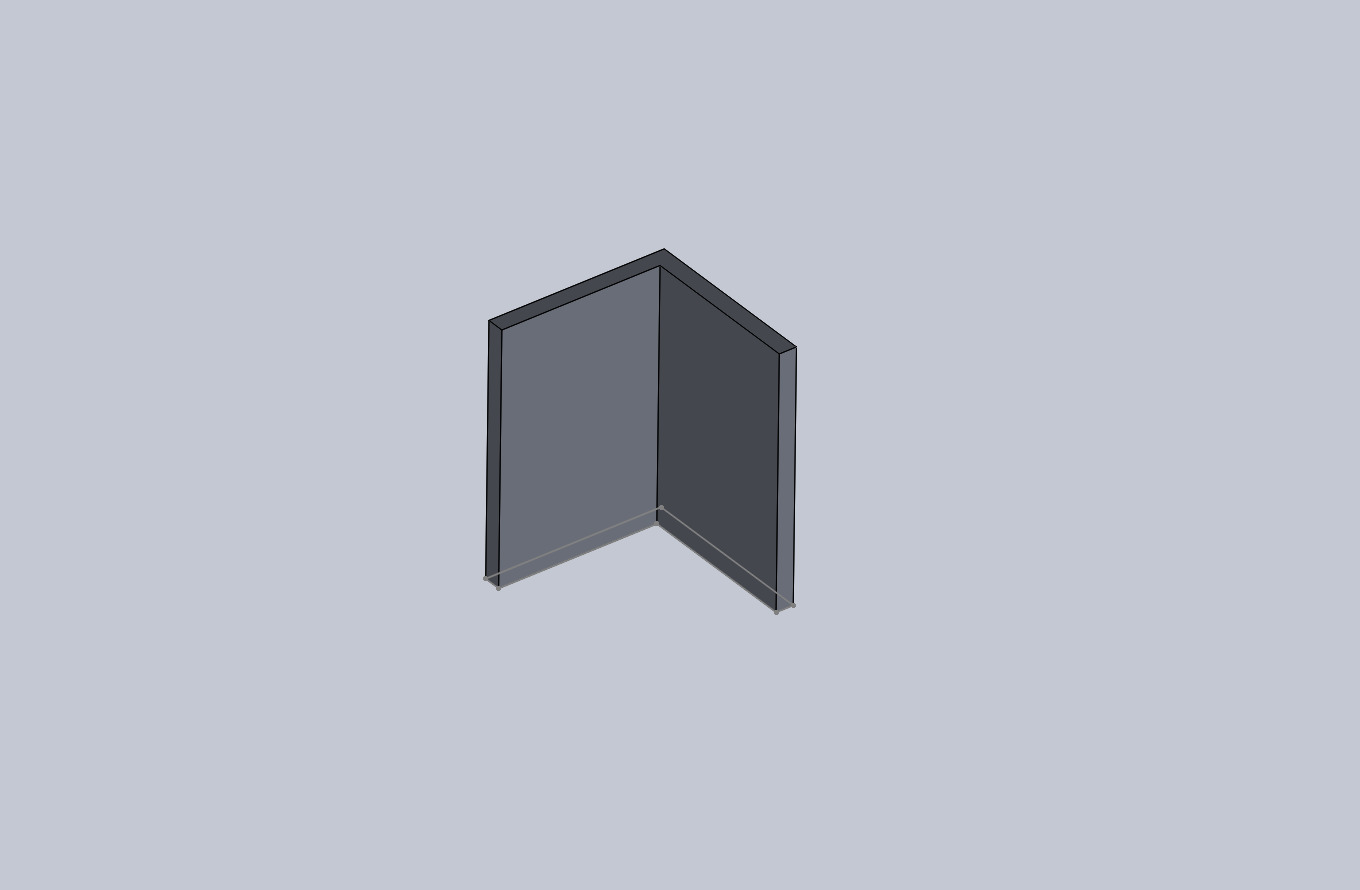
\includegraphics[width=0.5\linewidth]{Angulo aluminio.JPG}
    \caption{Perfil angular de aluminio utilizado como base estructural del módulo.}
    \label{fig:perfil_angular_aluminio}
\end{figure}


\subsubsection{Soporte del motor}
Se conservó el motor NEMA 17 de la configuración original. A partir de sus dimensiones se diseñó un soporte para fijarlo a la base estructural y mantener su alineación con el extrusor MK8. Debido a que el motor y el mecanismo de alimentación se desplazan junto con el carro del eje X, la configuración corresponde a un sistema de extrusión directa. La interfaz diseñada se muestra en la Figura~\ref{fig:soporte_extrusor}.

\begin{figure}[H]
    \centering
    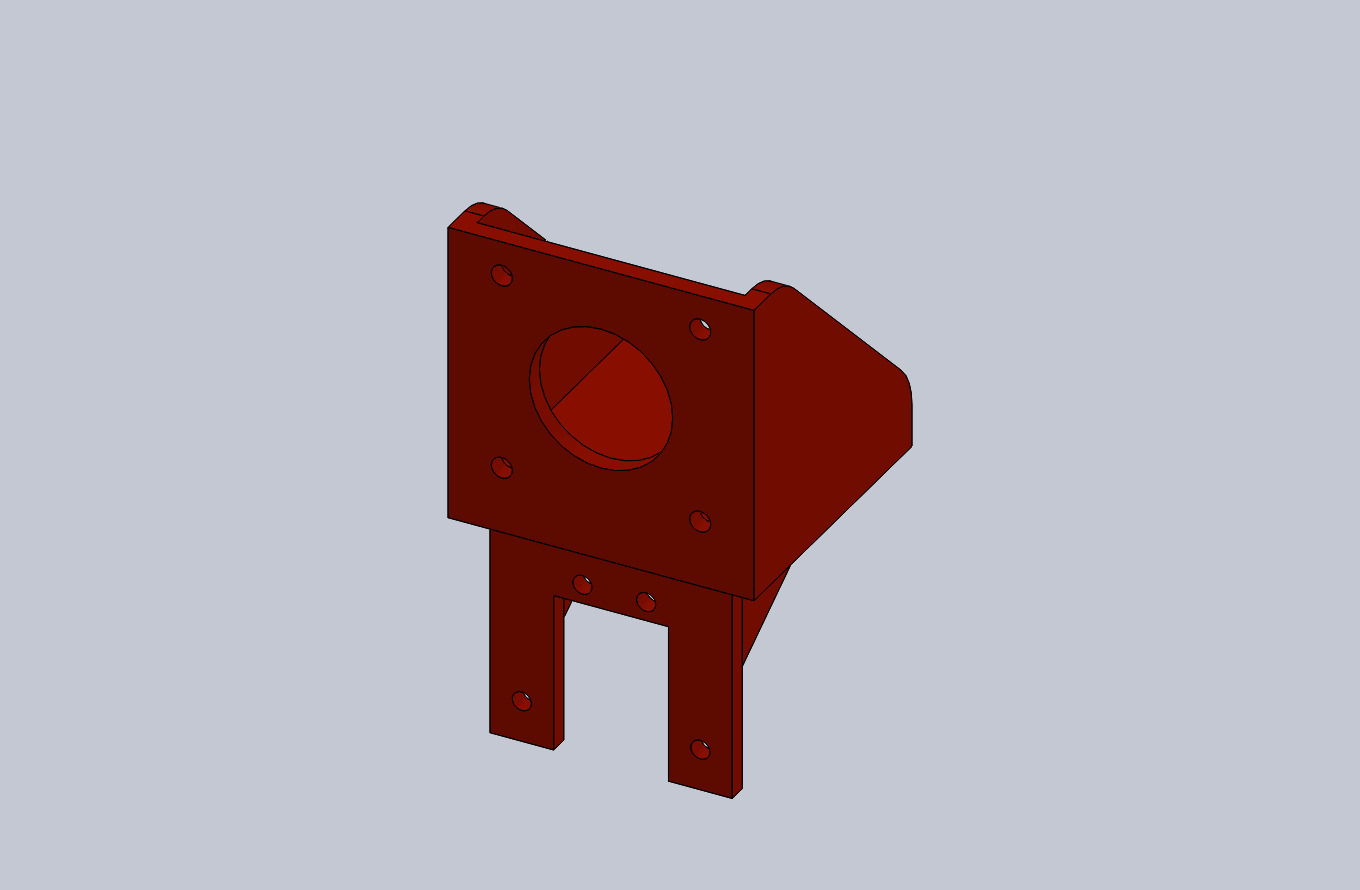
\includegraphics[width=0.5\linewidth]{Soporte ExtrusorV2.JPG}
    \caption{Soporte e interfaz diseñados para el extrusor MK8}
    \label{fig:soporte_extrusor}
\end{figure}
 
\subsubsection{Enfriador de hotend}
\label{subsec:enfriador_hotend}
Para limitar la propagación de calor hacia la zona fría del hotend se diseñó un conducto que dirige aire forzado sobre el disipador. La geometría se definió de manera que el flujo alcanzara las superficies del disipador sin interferir con el desplazamiento de los ejes ni con el sistema independiente de enfriamiento de capa.

\begin{figure}[H]
    \centering
    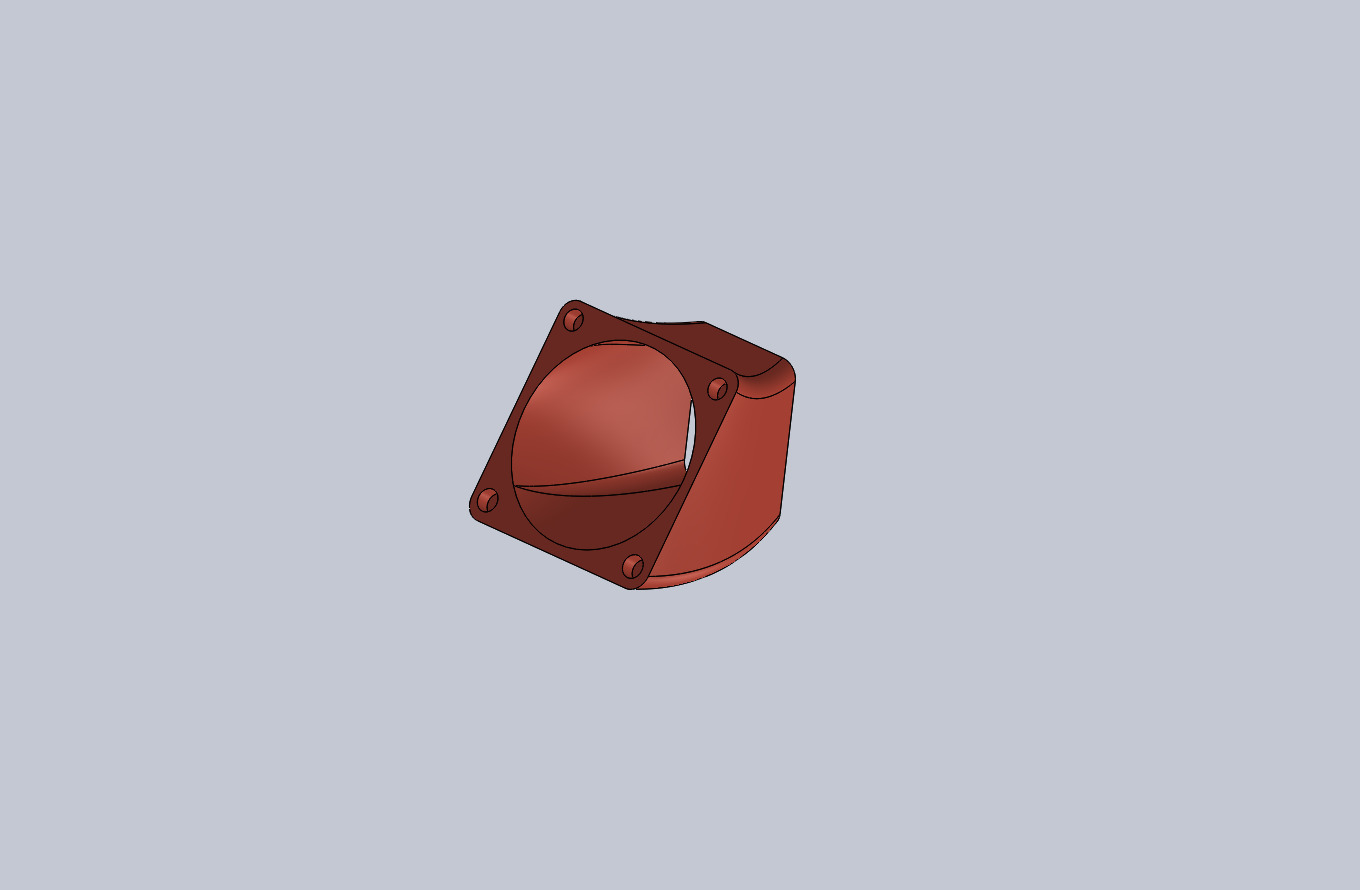
\includegraphics[width=0.5\linewidth]{Enfriador _HotendV2.JPG}
    \caption{Conducto diseñado para el enfriamiento del disipador del hotend.}
    \label{fig:enfriador_hotend}
\end{figure}

\subsubsection{Sistema de enfriamiento de capa}
\label{subsec:enfriamiento_capa}
La configuración original no disponía de ventilación dirigida hacia el material recién depositado Figura~\ref{fig:enfriador_capa}. Por ello se desarrolló un sistema independiente de enfriamiento de capa formado por un ventilador radial de 12 V y un conducto con dos salidas. La geometría dirige el aire hacia la región próxima a la boquilla desde dos lados, procurando evitar la incidencia directa sobre el bloque calefactor.

\begin{figure}[H]
    \centering
    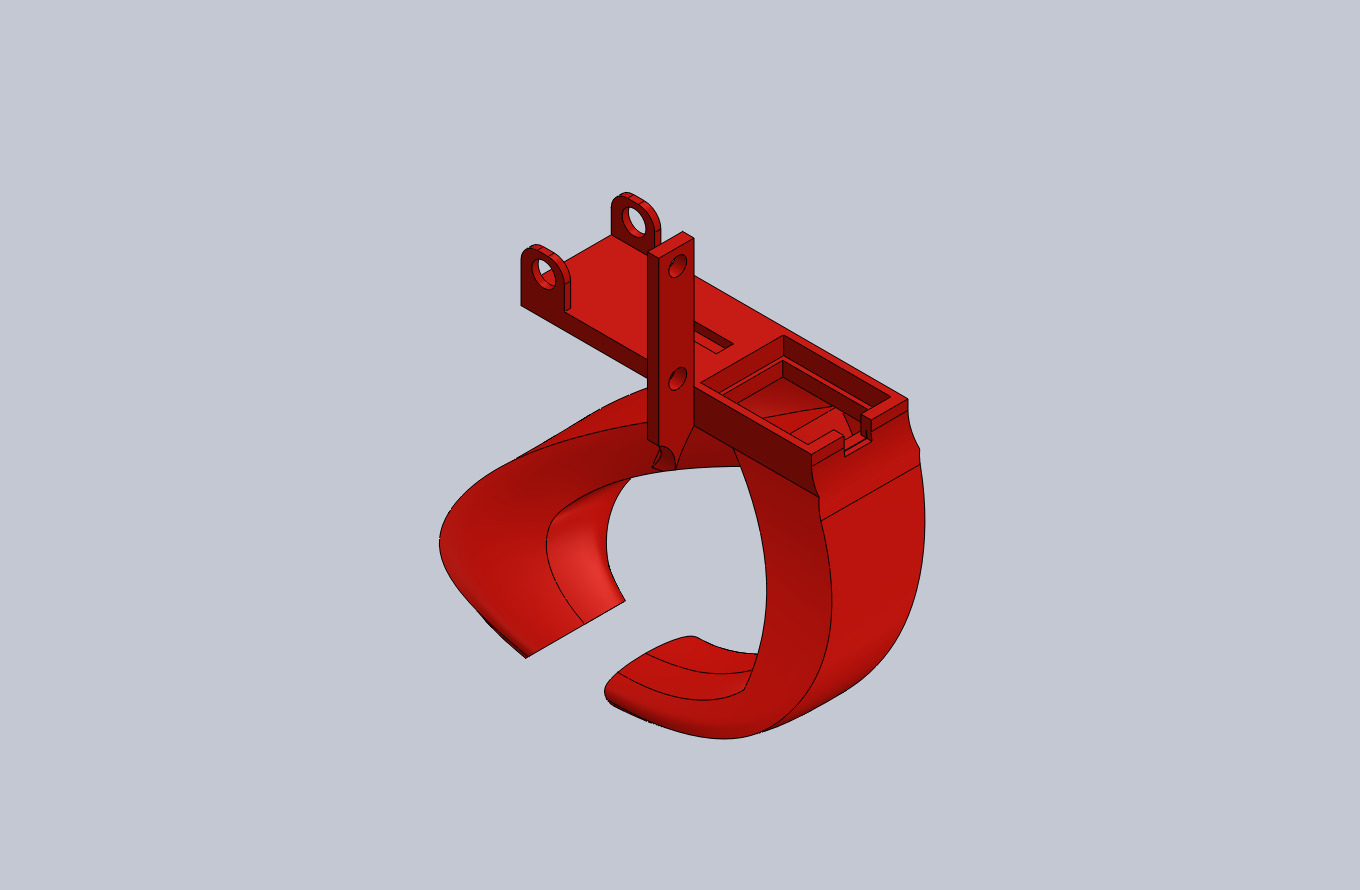
\includegraphics[width=0.5\linewidth]{enfriador de capa2.JPG}
    \caption{Diseño del sistema de enfriamiento de capa}
    \label{fig:enfriador_capa}
\end{figure}

\subsubsection{Modelado y ensamblaje virtual}
Una vez definidos los componentes se realizó un ensamblaje virtual del módulo en SolidWorks. El modelo integró la base de aluminio, el motor, el extrusor MK8, el hotend y ambos sistemas de ventilación. Esta etapa se utilizó para comprobar la posición relativa de los elementos, la alineación del recorrido del filamento y las separaciones necesarias antes de la fabricación e integración física. La
configuración obtenida se muestra en la Figura~\ref{fig:ensamblaje_final_extrusor}.

\begin{figure}[H]
    \centering
    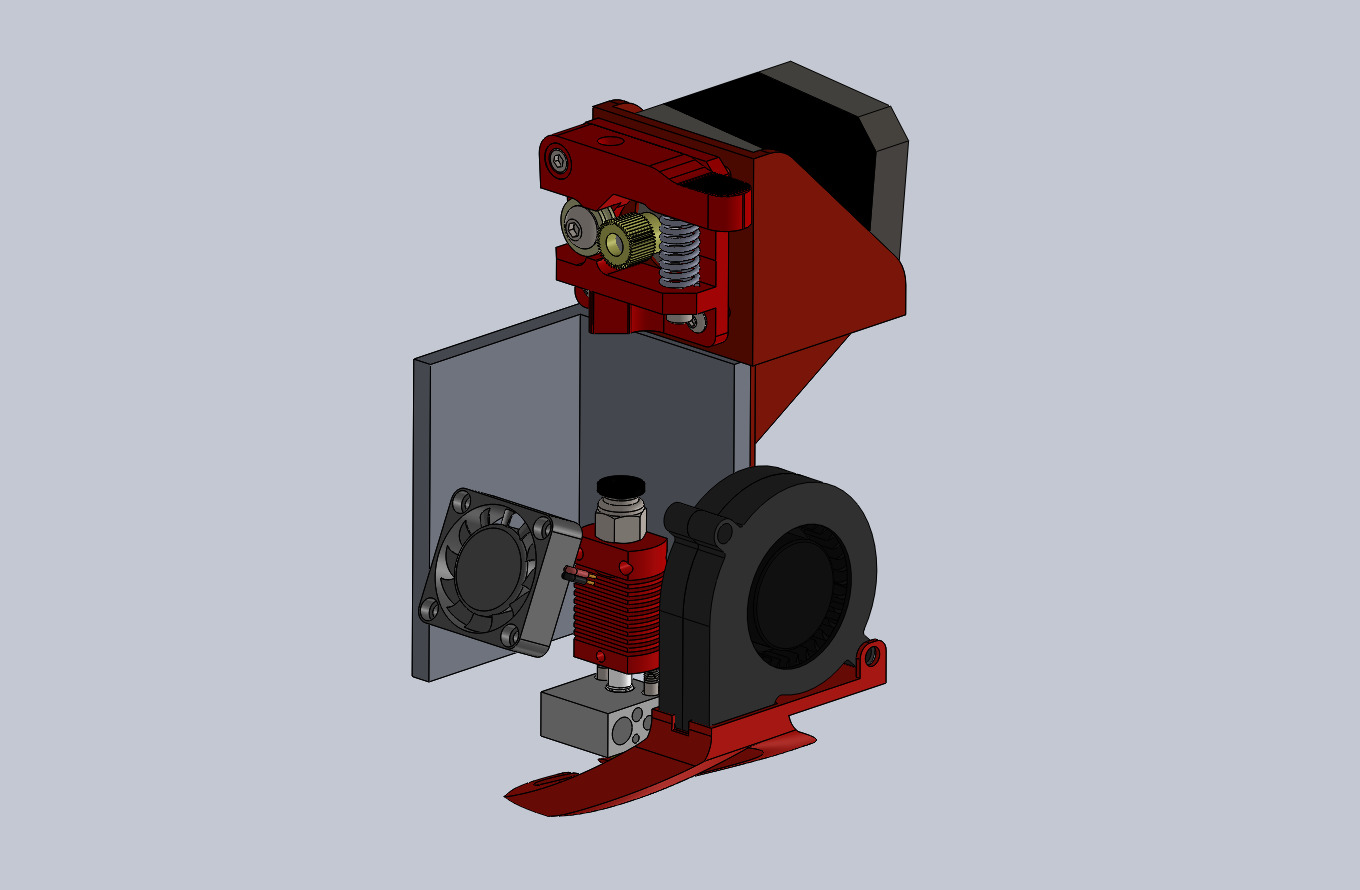
\includegraphics[width=0.5\linewidth]{ensamblaje_final_extrusor.jpg}
    \caption{Ensamble virtual del módulo de extrusión}
    \label{fig:ensamblaje_final_extrusor}
\end{figure}


\subsection{Diseño de componentes auxiliares}
El diagnóstico también mostró limitaciones mecánicas no asociadas directamente con el hotend. Para atenderlas se diseñaron piezas auxiliares orientadas a incrementar la rigidez de determinadas uniones y facilitar los procedimientos de ajuste. Estos componentes se modelaron en SolidWorks y se fabricaron en PLA mediante FDM.

\subsubsection{Escuadras de refuerzo}
En algunas uniones de los perfiles de aluminio se observó juego mecánico. Se diseñaron escuadras de refuerzo para instalarse en los puntos identificados como menos rígidos. La geometría empleada se muestra en la Figura~\ref{fig:estabilizador}.

\begin{figure}[H]
    \centering
    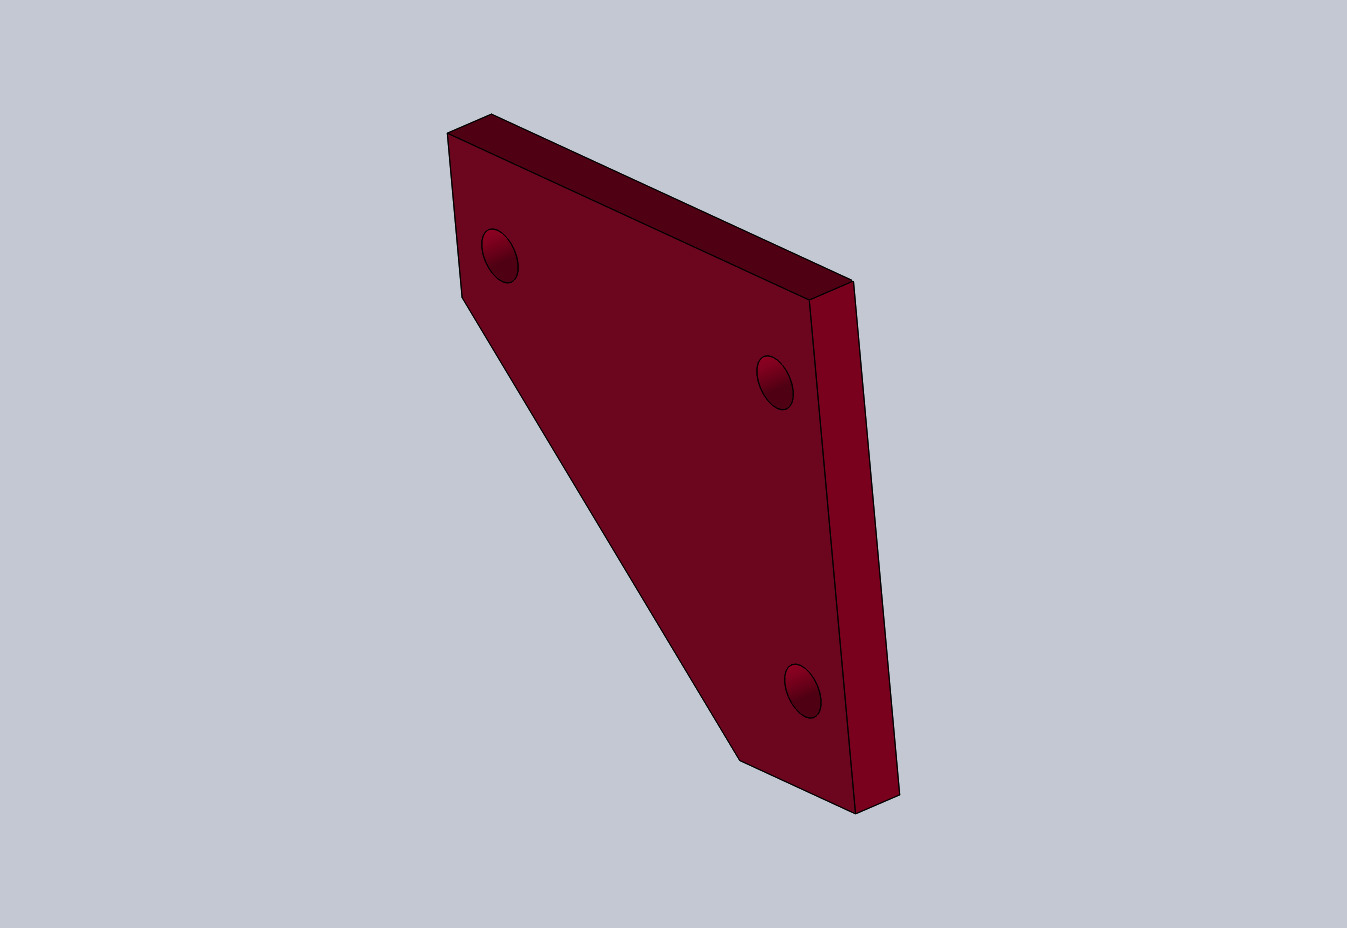
\includegraphics[width=0.5\linewidth]{estabilizador.JPG}
    \caption{Escuadra de refuerzo diseñada para la estructura.}
    \label{fig:estabilizador}
\end{figure}

\subsubsection{Tensor de la correa del eje X}
El ajuste original de la correa del eje X requería modificar manualmente su posición durante el ensamblaje. Para facilitar esta operación se desarrolló un tensor ajustable que permite variar la tensión con el sistema ya montado. La geometría se adaptó a las dimensiones de la plataforma a partir de mecanismos utilizados en proyectos de hardware abierto \cite{placeholder_proyecto_open_source}. El mecanismo diseñado se muestra en la Figura~\ref{fig:tensor_eje_x}.

\begin{figure}[H]
    \centering
    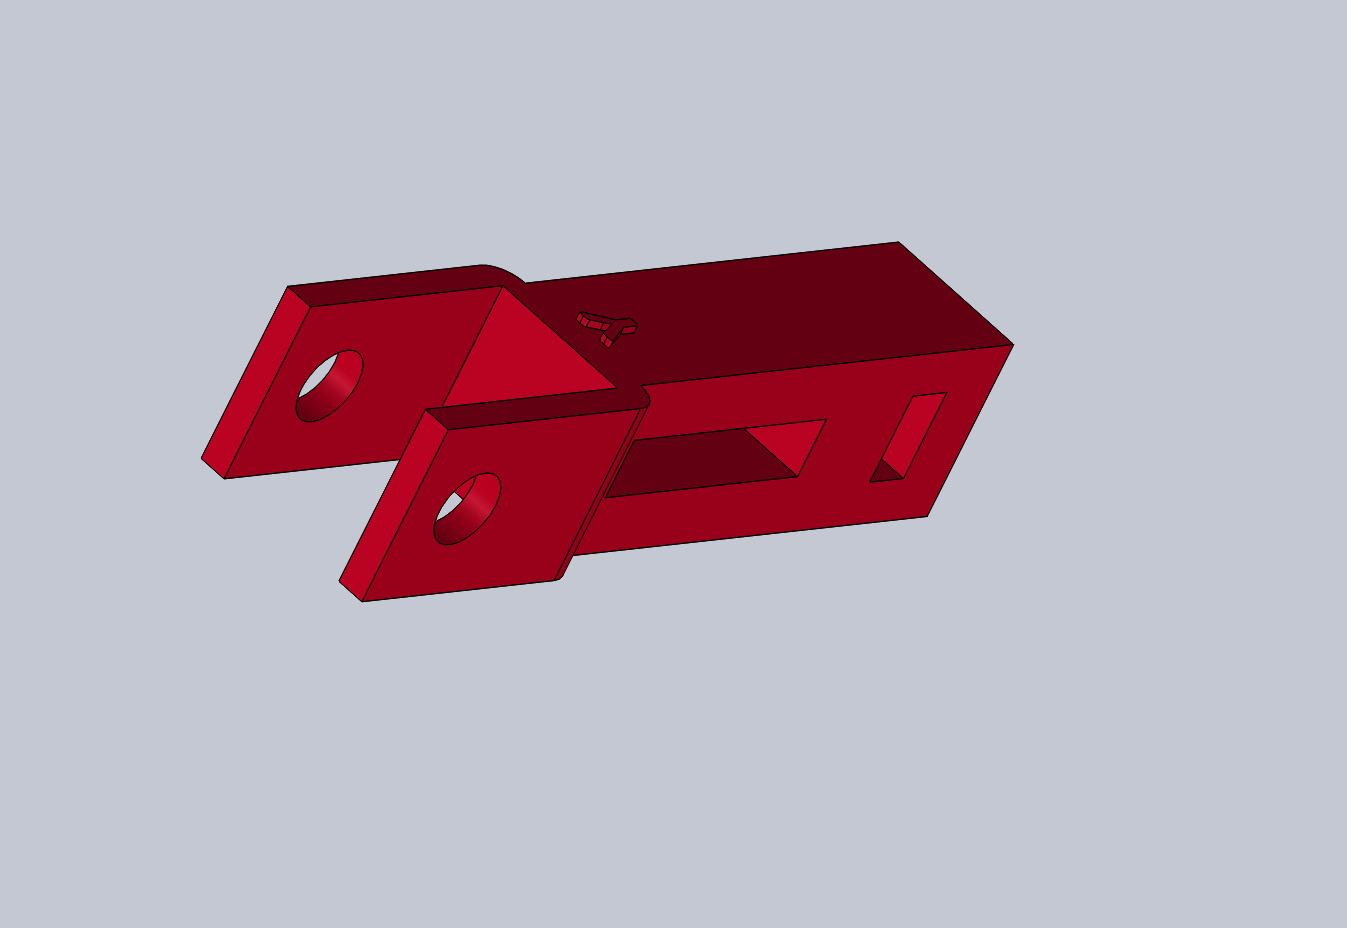
\includegraphics[width=0.5\linewidth]{Estructura de rodamiento Y.JPG}
    \caption{Tensor Eje X}
    \label{fig:tensor_eje_x}
\end{figure}

\subsubsection{Sistema de ajuste para finales de carrera}
También se diseñó un soporte ajustable para los interruptores de límite. El objetivo fue permitir el reposicionamiento del sensor sin desmontar elementos estructurales, de modo que la referencia de origen pudiera corregirse durante la calibración y el mantenimiento. El mecanismo diseñado se muestra en la Figura~\ref{fig:calibrador_altura}.

\begin{comment}
    Como solución se desarrolló un mecanismo de ajuste que permite modificar la posición de los finales de carrera sin necesidad de desmontar componentes estructurales. Este sistema facilita la calibración inicial de la máquina y permite realizar correcciones posteriores de manera rápida y repetible.

La implementación de este elemento contribuyó a mejorar la precisión del proceso de homing y redujo significativamente el tiempo requerido para la puesta en marcha del sistema.
\end{comment}


\begin{figure}[H]
    \centering
    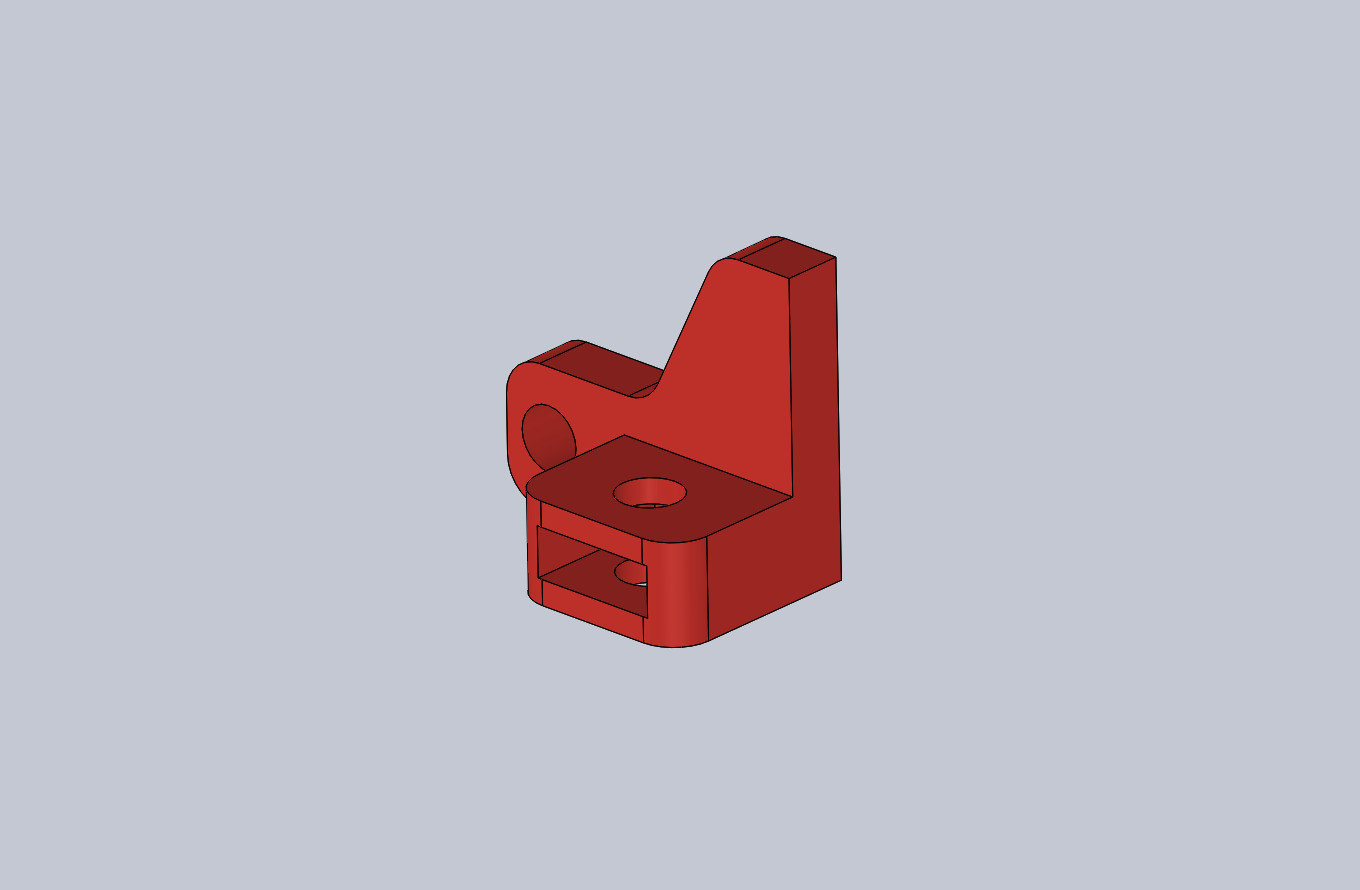
\includegraphics[width=0.5\linewidth]{Calibrador de altura.JPG}
    \caption{Sistema de ajuste para finales de carrera}
    \label{fig:calibrador_altura}
\end{figure}


%%%%%%%%%%%%%%%%%%%%%%%%%%%%%%%%%%%%%%%%%%%%%%%%%%%%%%%%%%%%%%%%%%%%%%%%%%%%%%%%%%%%%%%%%%%%%%%%%%%%%%%%%%%%%%%%%%%%%%%%%%%%%%%%%%%%%%%%%%%%%%%%%%%%%%%%%%%%%%%%%%%%%%%%%%%%%%%%%%%%%%%%%%%%%%%%%%%%%%%%%%%%%%%%%%%%%%%%%%%%%%%%%%%%%%%%%%%%%%%%%%%%%%%%%%%%%%%%%%%%%%%%%%%%%%%%%%%%%%%%%%%%%%%%%%%%%%%%%%%%%%%%%%%%%%%%%%%%%%%%%%%%%%%%%%%%

\section{Materiales y métodos de fabricación}
\subsection{Componentes principales}
Los componentes empleados para la integración de la plataforma se presentan en la Tabla~\ref{tab:materiales_componentes}. La selección del hotend y del sistema de alimentación respondió a su compatibilidad con filamento de \SI{1.75}{\milli\metre}, disponibilidad comercial y facilidad de reemplazo.
\begin{table}[htbp]
    \centering
    \small % Disminuye un poco la fuente para evitar desbordamientos
    \caption{Materiales y componentes utilizados en la fabricación de la impresora.}
    \label{tab:materiales_componentes}
    % \textwidth fuerza a la tabla a no salirse del margen de la página
    \begin{tabularx}{\textwidth}{>{\raggedright\arraybackslash}p{3.8cm} Y l}
        \toprule
        \textbf{Componente} & \textbf{Especificación} & \textbf{Cantidad} \\
        \midrule
        Microcontrolador & Arduino Mega & 1 pza. \\
        Placa de potencia & RAMPS 1.4 & 1 pza. \\
        Motores paso a paso & NEMA 17 (\qty{1.7}{\A}) & 4 pzas. \\
        Cables para motor & Longitud de \qty{1}{\m} & 4 pzas. \\
        Hotend & Ender Creality CR-10, boquilla \qty{0.4}{\mm}, filamento \qty{1.75}{\mm} & 1 pza. \\
        Cama caliente & Dimensión \qty{214}{\mm} $\times$ \qty{214}{\mm}; \qty{12}{\V} / \qty{24}{\V} & 1 pza. \\
        Fuente de poder & \qty{12}{\V} - \qty{30}{\A} (\qty{360}{\W}) & 1 pza. \\
        Controlador de motor & A4988 con disipador térmico & 4 pzas. \\
        Ventilador & \qty{12}{\V}, \qty{40}{\mm} & 2 pzas. \\
        Extrusor & Ender Creality CR-10S & 1 pza. \\
        Resortes para cama & Acero; DE: \qty{9.8}{\mm}, DI: \qty{5.45}{\mm}, Altura: \qty{25.3}{\mm} & 4 pzas. \\
        Tubo de teflón & PTFE translúcido ID: \qty{2}{\mm}, OD: \qty{4}{\mm}, Longitud: \qty{2}{\m} & 1 pza. \\
        Microswitch endstop & Con cable conector, \qty{24}{\V}, \qty{1.6}{\mm} $\times$ \qty{3}{\mm} $\times$ \qty{4}{\mm} & 3 pzas. \\
        Banda dentada & GT2 \qty{6}{\mm} (\qty{1}{\m}) & 2 pzas. \\
        Polea dentada & GT2 20T para banda de \qty{6}{\mm} & 2 pzas. \\
        Termistor & NTC 100K con cable & 2 pzas. \\
        Tubo termorretráctil & Diámetros variados & 1 lote \\
        \bottomrule
    \end{tabularx}
\end{table}





\subsection{Fabricación de piezas poliméricas}

Las piezas de geometría específica se fabricaron mediante FDM utilizando la impresora rehabilitada. Los modelos CAD se exportaron en formato STL y se procesaron en Ultimaker Cura 5.12. Se utilizó filamento PLA de 1.75 mm y boquilla de 0.4 mm.

La orientación de cada pieza se seleccionó considerando las superficies de apoyo, la geometría y la dirección principal de las cargas durante su funcionamiento. Cuando la geometría lo requirió se utilizaron estructuras de soporte. Después de la impresión se inspeccionaron las piezas para detectar deformaciones, separación entre capas o formación excesiva de hilos; posteriormente se retiraron soportes y se limpiaron las superficies y orificios destinados al montaje.

Los valores definitivos de altura de capa, temperatura de extrusión, temperatura de cama y patrón de relleno deben registrarse a partir de los archivos de laminado empleados durante la fabricación. No se incorporan valores no documentados en los registros del proyecto. La densidad de relleno registrada para las piezas finales fue de 40 $\%$ y la velocidad de impresión de 50 mm/s.

\subsection{Fabricación de la base metalica}

La base estructural del módulo se fabricó a partir de un perfil angular de aluminio de 4 mm de espesor. Se cortó una sección de 100 mm y posteriormente se trazaron y perforaron los puntos de montaje correspondientes a tornillos M3. Después del corte y perforado se eliminaron rebabas y se ajustaron los bordes mediante esmerilado. Antes del montaje final se verificó la correspondencia de los orificios con el motor, el hotend y los soportes.

\subsection{Integración del módulo de extrusión }

La base de aluminio se instaló sobre el carro del eje X. Sobre ella se montaron el motor NEMA 17, el mecanismo MK8 y el hotend, verificando la alineación del recorrido del filamento. Posteriormente se instalaron el ventilador axial destinado al disipador del hotend y el ventilador radial utilizado para el enfriamiento de capa, junto con sus respectivos conductos.

También se incorporaron el cartucho calefactor, el termistor y los conductores eléctricos necesarios para la conexión con la tarjeta de control. Antes de energizar los calentadores se verificó manualmente el avance del filamento, la sujeción de los componentes y la ausencia de interferencias entre el módulo y la estructura durante el desplazamiento del carro.

\section{Configuración y calibración}

Concluido el ensamblaje se configuró el sistema de control y se calibraron los mecanismos de movimiento, la alimentación de filamento y el control térmico. Estas actividades se realizaron antes de las pruebas de impresión con el propósito de establecer parámetros de operación reproducibles.

\subsection{Configuración del firmware REVISAR}
La electrónica utiliza un Arduino Mega con tarjeta RAMPS 1.4. Sobre esta plataforma se instaló Marlin 2.1.2.1 \cite{marlinfw} y se configuraron desde cero los parámetros correspondientes a los ejes X, Y y Z, el extrusor, los sensores de temperatura, los calentadores, los ventiladores y los interruptores de límite.

Los valores iniciales de pasos por unidad se calcularon a partir de las características de los motores y de los mecanismos de transmisión. Antes de activar los calentadores se comprobaron individualmente los movimientos de los ejes, verificando el sentido de desplazamiento, la actuación de los finales de carrera y la ausencia de interferencias mecánicas.

\subsection{Calibración del sistema de movimiento}
\label{sec:calibracion_del_sistema_de_movimiento}

Para verificar la correspondencia entre desplazamiento programado y desplazamiento real se realizaron pruebas independientes en X, Y y Z. En cada eje se ordenaron diez desplazamientos consecutivos de 10 mm en el mismo sentido, equivalentes a 100 mm programados. La distancia total recorrida se midió y se comparó con la solicitada.
Cuando se detectó una diferencia, el parámetro de pasos por milímetro se corrigió mediante la relación:

\begin{equation}
E_{\mathrm{nuevo}} = E_{\mathrm{actual}} \cdot 
\frac{L_{\mathrm{programada}}}{L_{\mathrm{medida}}}
\label{eq:pasos_mm_movimiento}
\end{equation}



donde $E_{\mathrm{nuevo}}$ corresponde al nuevo valor de pasos por milímetro 
del eje, $E_{\mathrm{actual}}$ al valor utilizado durante la prueba, 
$L_{\mathrm{programada}}$ a la distancia solicitada y $L_{\mathrm{medida}}$ a 
la distancia realmente recorrida. Los valores finales y el
error medido se presentan en el capítulo de resultados.

\subsection{Calibración del extrusor}
\label{sec:calibracion_extrusor}
La calibración del extrusor se realizó para establecer la correspondencia entre la longitud de filamento solicitada y la longitud realmente suministrada. Para aislar la respuesta del mecanismo de alimentación se retiró el hotend durante esta prueba. Se marcó una referencia sobre el filamento y se ordenaron diez desplazamientos de 10 mm, equivalentes a una alimentación total programada de 100 mm.

La longitud desplazada se midió desde la referencia inicial y el valor de pasos por milímetro se corrigió mediante la ecuación~\ref{eq:pasos_mm_movimiento}, sustituyendo el desplazamiento del eje por la longitud de filamento. Después de incorporar el nuevo valor al firmware se realizó una prueba adicional de verificación.

\subsection{Ajuste del control térmico}
\label{sec:calibracion_termica}
La regulación térmica se ajustó para el hotend y la cama calefactada utilizando la función de autosintonización PID disponible en Marlin. El procedimiento se ejecutó de manera independiente para cada elemento a las temperaturas de operación utilizadas para PLA. Las constantes obtenidas se incorporaron a la configuración del firmware.

Después de la sintonización se verificó el comportamiento térmico durante la operación de la impresora. Las constantes finales, las temperaturas alcanzadas, los tiempos de calentamiento y la variación en estado estable se presentan en el capítulo de resultados.

\section{Protocolo de evacuación experimental}
Una vez configurada y calibrada la plataforma se estableció un conjunto de pruebas para evaluar el sistema final. Los resultados se reservan para el capítulo siguiente; en esta sección se definen únicamente las variables y procedimientos de medición.

\subsection{Evaluación del posicionamiento y la extrusión}
La precisión de movimiento se evaluó comparando distancias programadas con distancias medidas en cada eje. Para el extrusor se comparó una longitud programada de filamento con la longitud efectivamente suministrada. En ambos casos se calculó el error absoluto y el error relativo porcentual respecto al valor programado. 

\subsection{Evacuación térmica}
Para el hotend y la cama se registraron la temperatura programada, la temperatura alcanzada, el tiempo necesario para alcanzar la condición de operación y la variación observada una vez alcanzado el régimen estable. Para evaluar el sistema de disipación del hotend se realizaron mediciones de temperatura en el disipador manteniendo constante la temperatura del bloque calefactor y modificando la configuración de ventilación. La posición del sensor se mantuvo fija entre pruebas para conservar condiciones comparables.

\subsection{Evaluación dimensional y de calidad de impresión}
La precisión dimensional se evaluó mediante piezas de geometría conocida. Las dimensiones obtenidas se midieron sobre los ejes X, Y y Z y se compararon con las dimensiones nominales del modelo. El análisis se complementó con una inspección visual de defectos de impresión, incluyendo presencia de hilos, deformación de la base y patrones asociados con vibración.

También se contemplaron pruebas geométricas destinadas a observar el comportamiento en voladizos, puentes y movimientos con retracción. Las condiciones de laminado utilizadas en cada ensayo deben mantenerse registradas para permitir una comparación reproducible entre las piezas.

\subsection{Evacuación económica}
La evaluación económica se planteó a partir del costo de los componentes utilizados en la construcción e integración de la plataforma. Para la comparación con alternativas comerciales se considerarán equipos con volumen de impresión y aplicación general comparables. El costo de mano de obra no se incorpora al costo de fabricación, ya que el diseño, ensamblaje y calibración fueron realizados por el autor como parte del trabajo académico. Los precios, modelos comerciales y fecha de consulta se presentan en el capítulo de resultados.

\section{Resumen del capitulo}
El procedimiento descrito permitió pasar de una plataforma fuera de servicio a una configuración rehabilitada, diagnosticada y posteriormente modificada mediante un proceso iterativo de diseño. Las intervenciones se concentraron en el módulo de extrusión, el manejo térmico, el enfriamiento de capa y los mecanismos auxiliares de ajuste. Después de la integración se configuraron y calibraron los subsistemas mecánicos, de extrusión y térmicos, y se definió un protocolo para evaluar el desempeño del sistema. El capítulo siguiente presenta los resultados obtenidos mediante estos procedimientos




\chapter{Resultados}
\section{Ensamblaje final del sistema}
Como resultado del proceso de diseño, fabricación y ensamblaje, se obtuvo el sistema de impresión 3D mostrado en la Figura \ref{fig:ensamblaje_final}. El equipo quedó conformado por la estructura de perfiles de aluminio, el sistema de movimiento cartesiano, el módulo de extrusión rediseñado y el sistema de control basado en Arduino Mega y RAMPS 1.4.

\begin{figure}[H]
    \centering
    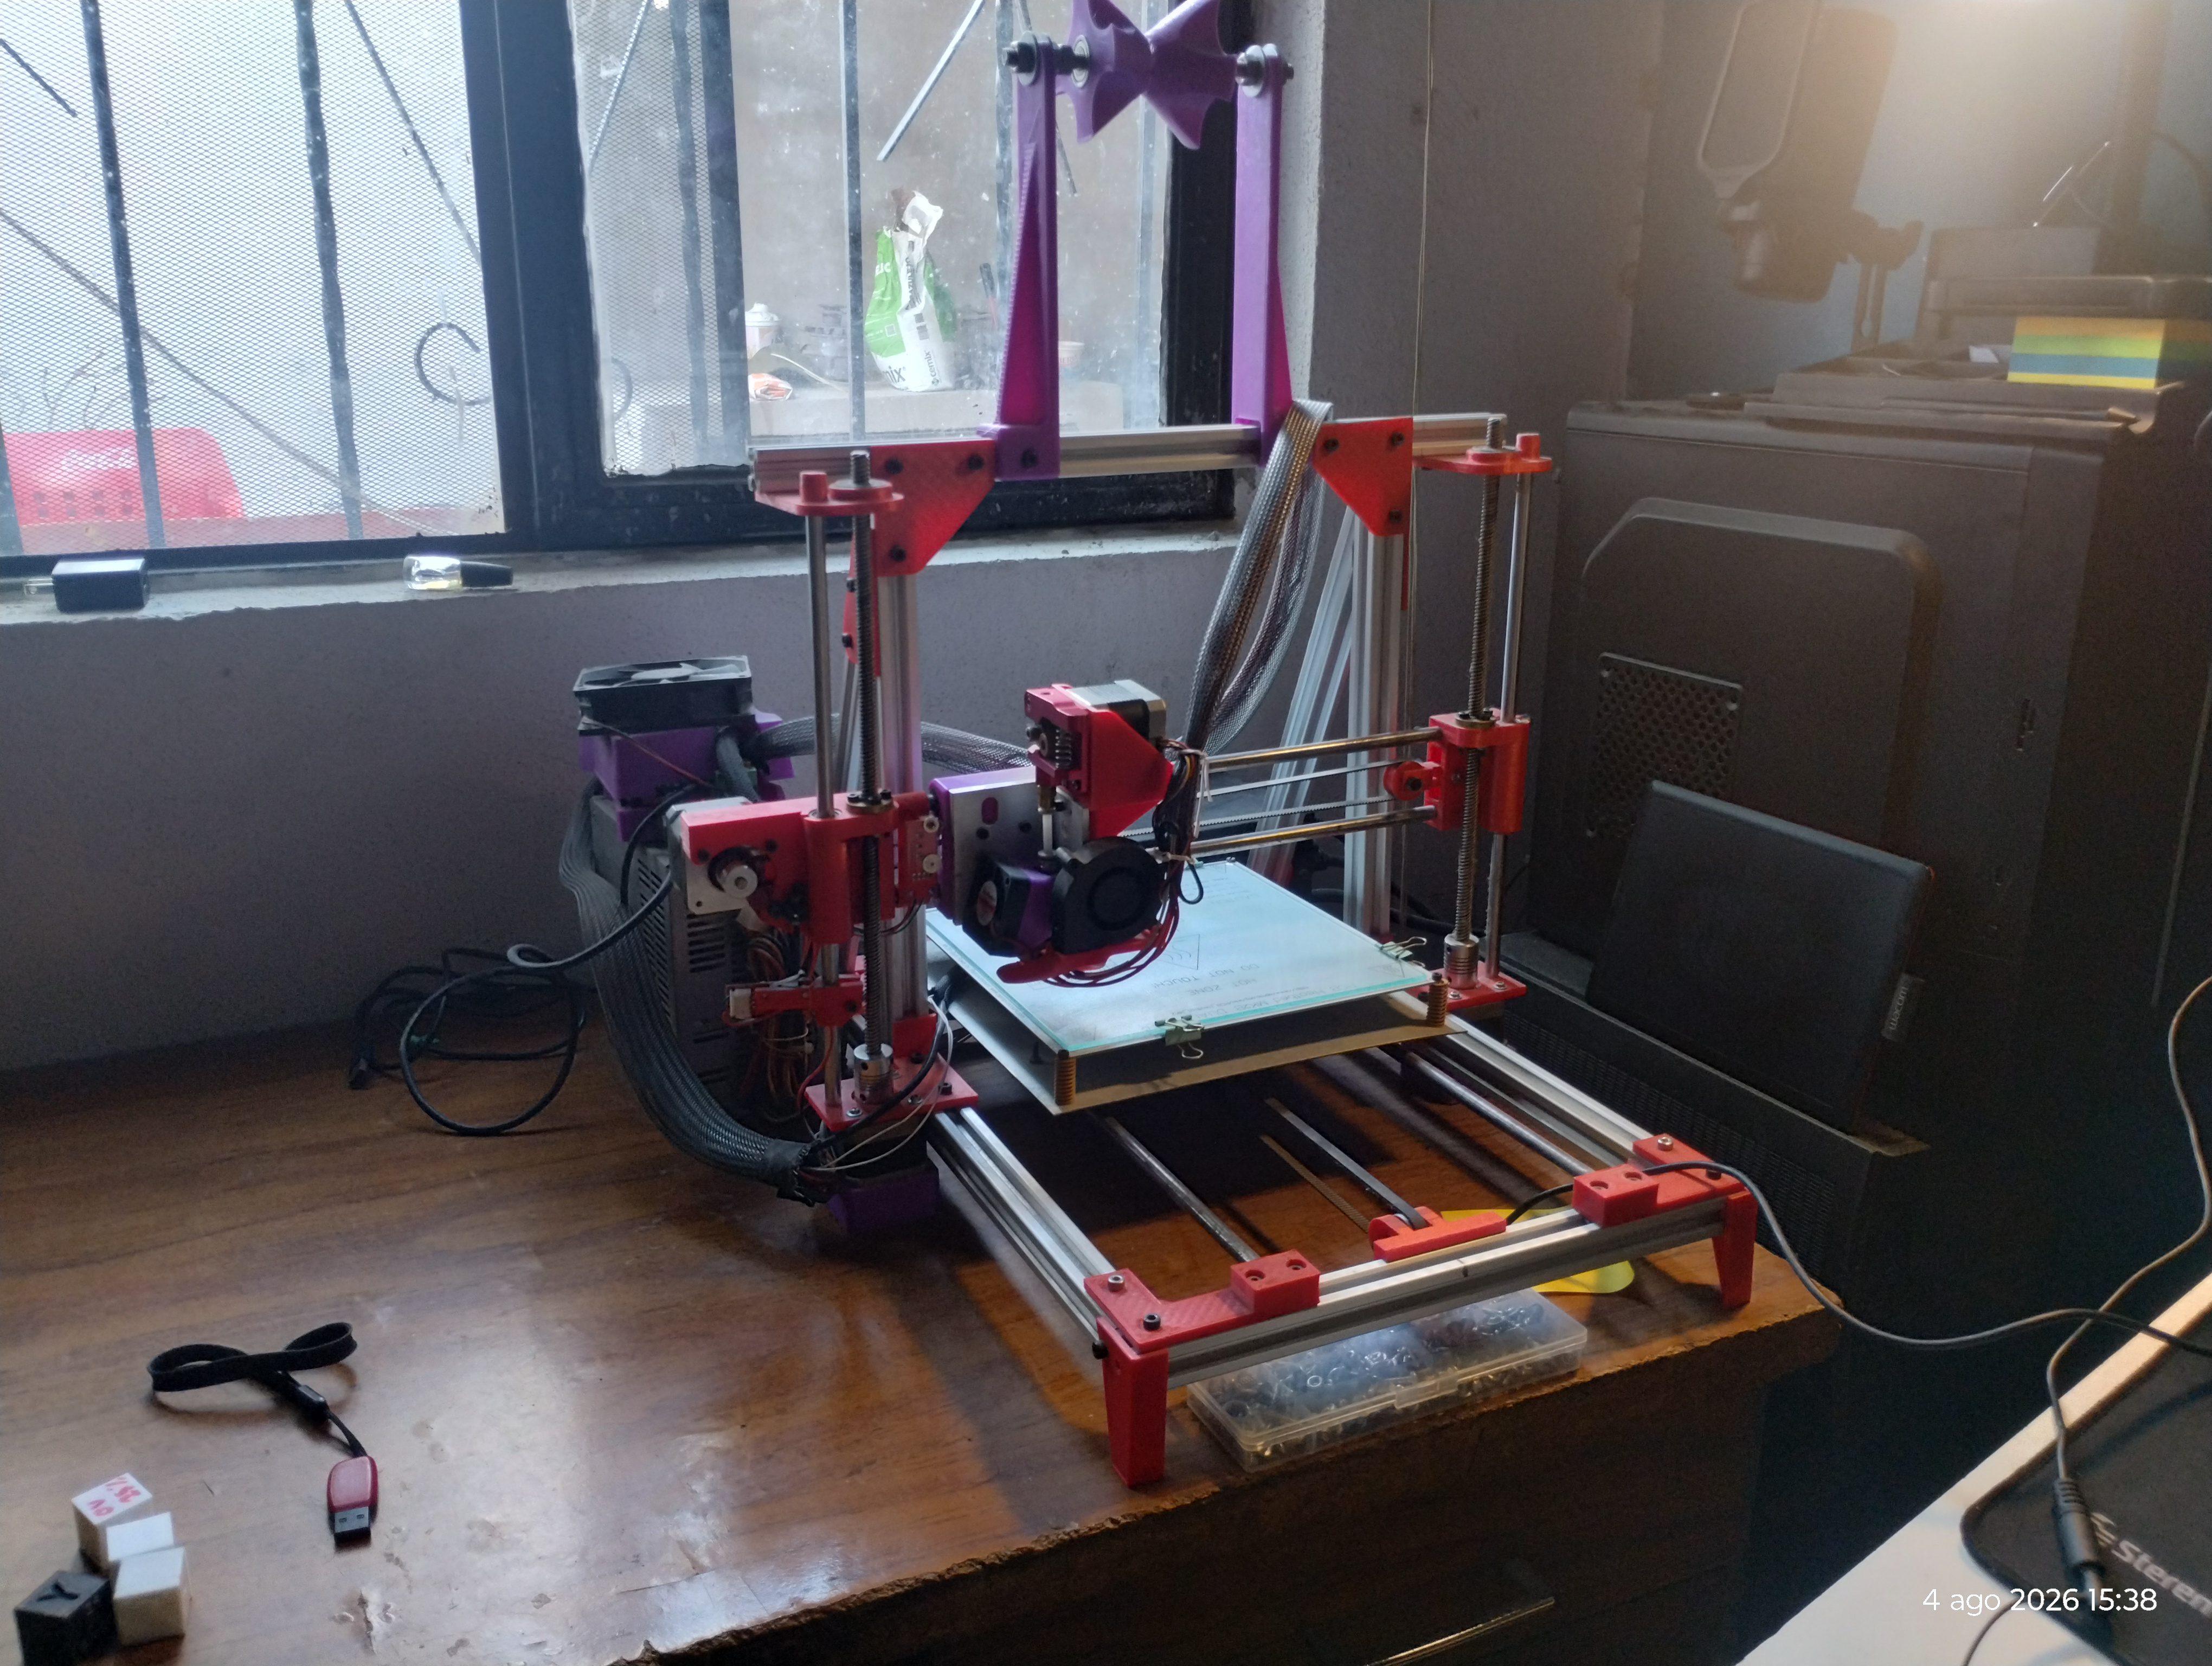
\includegraphics[width=0.5\linewidth]{Ensamblaje final.jpg}
    \caption{Ensamblaje final}
    \label{fig:ensamblaje_final}
\end{figure}

\subsection{Dimensiones y masa del equipo}
Las dimensiones generales y la masa total del equipo se presentan en la Tabla~\ref{tab:dimensiones_equipo}. Estos valores corresponden al equipo completamente ensamblado, incluyendo la estructura, la electrónica, el sistema de extrusión y la cama calefactada.

\begin{table}[htbp]
    \centering
    \caption{Dimensiones generales y masa total del equipo.}
    \label{tab:dimensiones_equipo}
    \begin{tabular}{lc}
        \toprule
        \textbf{Característica} & \textbf{Valor} \\
        \midrule
        Largo      & \qty{47}{\cm} \\
        Ancho      & \qty{52}{\cm} \\
        Alto       & \qty{57}{\cm} \\
        Masa total & \qty{7.2}{\kg} \\
        \bottomrule
    \end{tabular}
   
\end{table}

El equipo presenta dimensiones exteriores de \qty{47}{\cm} de largo, 
\qty{52}{\cm} de ancho y \qty{57}{\cm} de alto, con una masa total de 
\qty{7.2}{\kg}. Estas dimensiones permiten ubicar el equipo sobre una mesa 
de trabajo convencional y son compatibles con el espacio disponible en un 
laboratorio de prototipado.

\subsection{Componentes auxiliares integrados}

Además del módulo de extrusión, el equipo incorpora los siguientes 
componentes auxiliares:

\begin{itemize}
    \item \textbf{Escuadras de refuerzo:} instaladas en las uniones de menor 
    rigidez para reducir el juego mecánico (Figura~\ref{fig:estabilizador}).
    \item \textbf{Tensor de la correa del eje \(X\):} permite ajustar la 
    tensión de la correa después del ensamblaje 
    (Figura~\ref{fig:tensor_eje_x}).
    \item \textbf{Sistema de ajuste de finales de carrera:} permite 
    reposicionar los interruptores de límite sin desmontar la estructura 
    (Figura~\ref{fig:calibrador_altura}).
    \item \textbf{Soporte de carrete:} sostiene el carrete de filamento 
    durante la impresión.
    \item \textbf{Case del controlador:} protege la electrónica de control.
\end{itemize}


\section{Sistema de extrusión desarrollado}
\label{sec:sistema_extrusion_desarrollado}
Como resultado del proceso de diseño y fabricación, se obtuvo el módulo de extrusión mostrado en la Figura~\ref{fig:extrusor_final}, correspondiente a la configuración final integrada en la impresora. El módulo integró la base estructural de aluminio, el motor NEMA 17, el extrusor MK8, el hotend y los dos sistemas de enfriamiento del hotend y capa. La configuración corresponde a un sistema de accionamiento directo (\textit{direct drive}), en el que el motor y el mecanismo de alimentación se desplazan junto con el hotend sobre el carro del eje \(X\).
 

\begin{figure}[H]
    \centering
    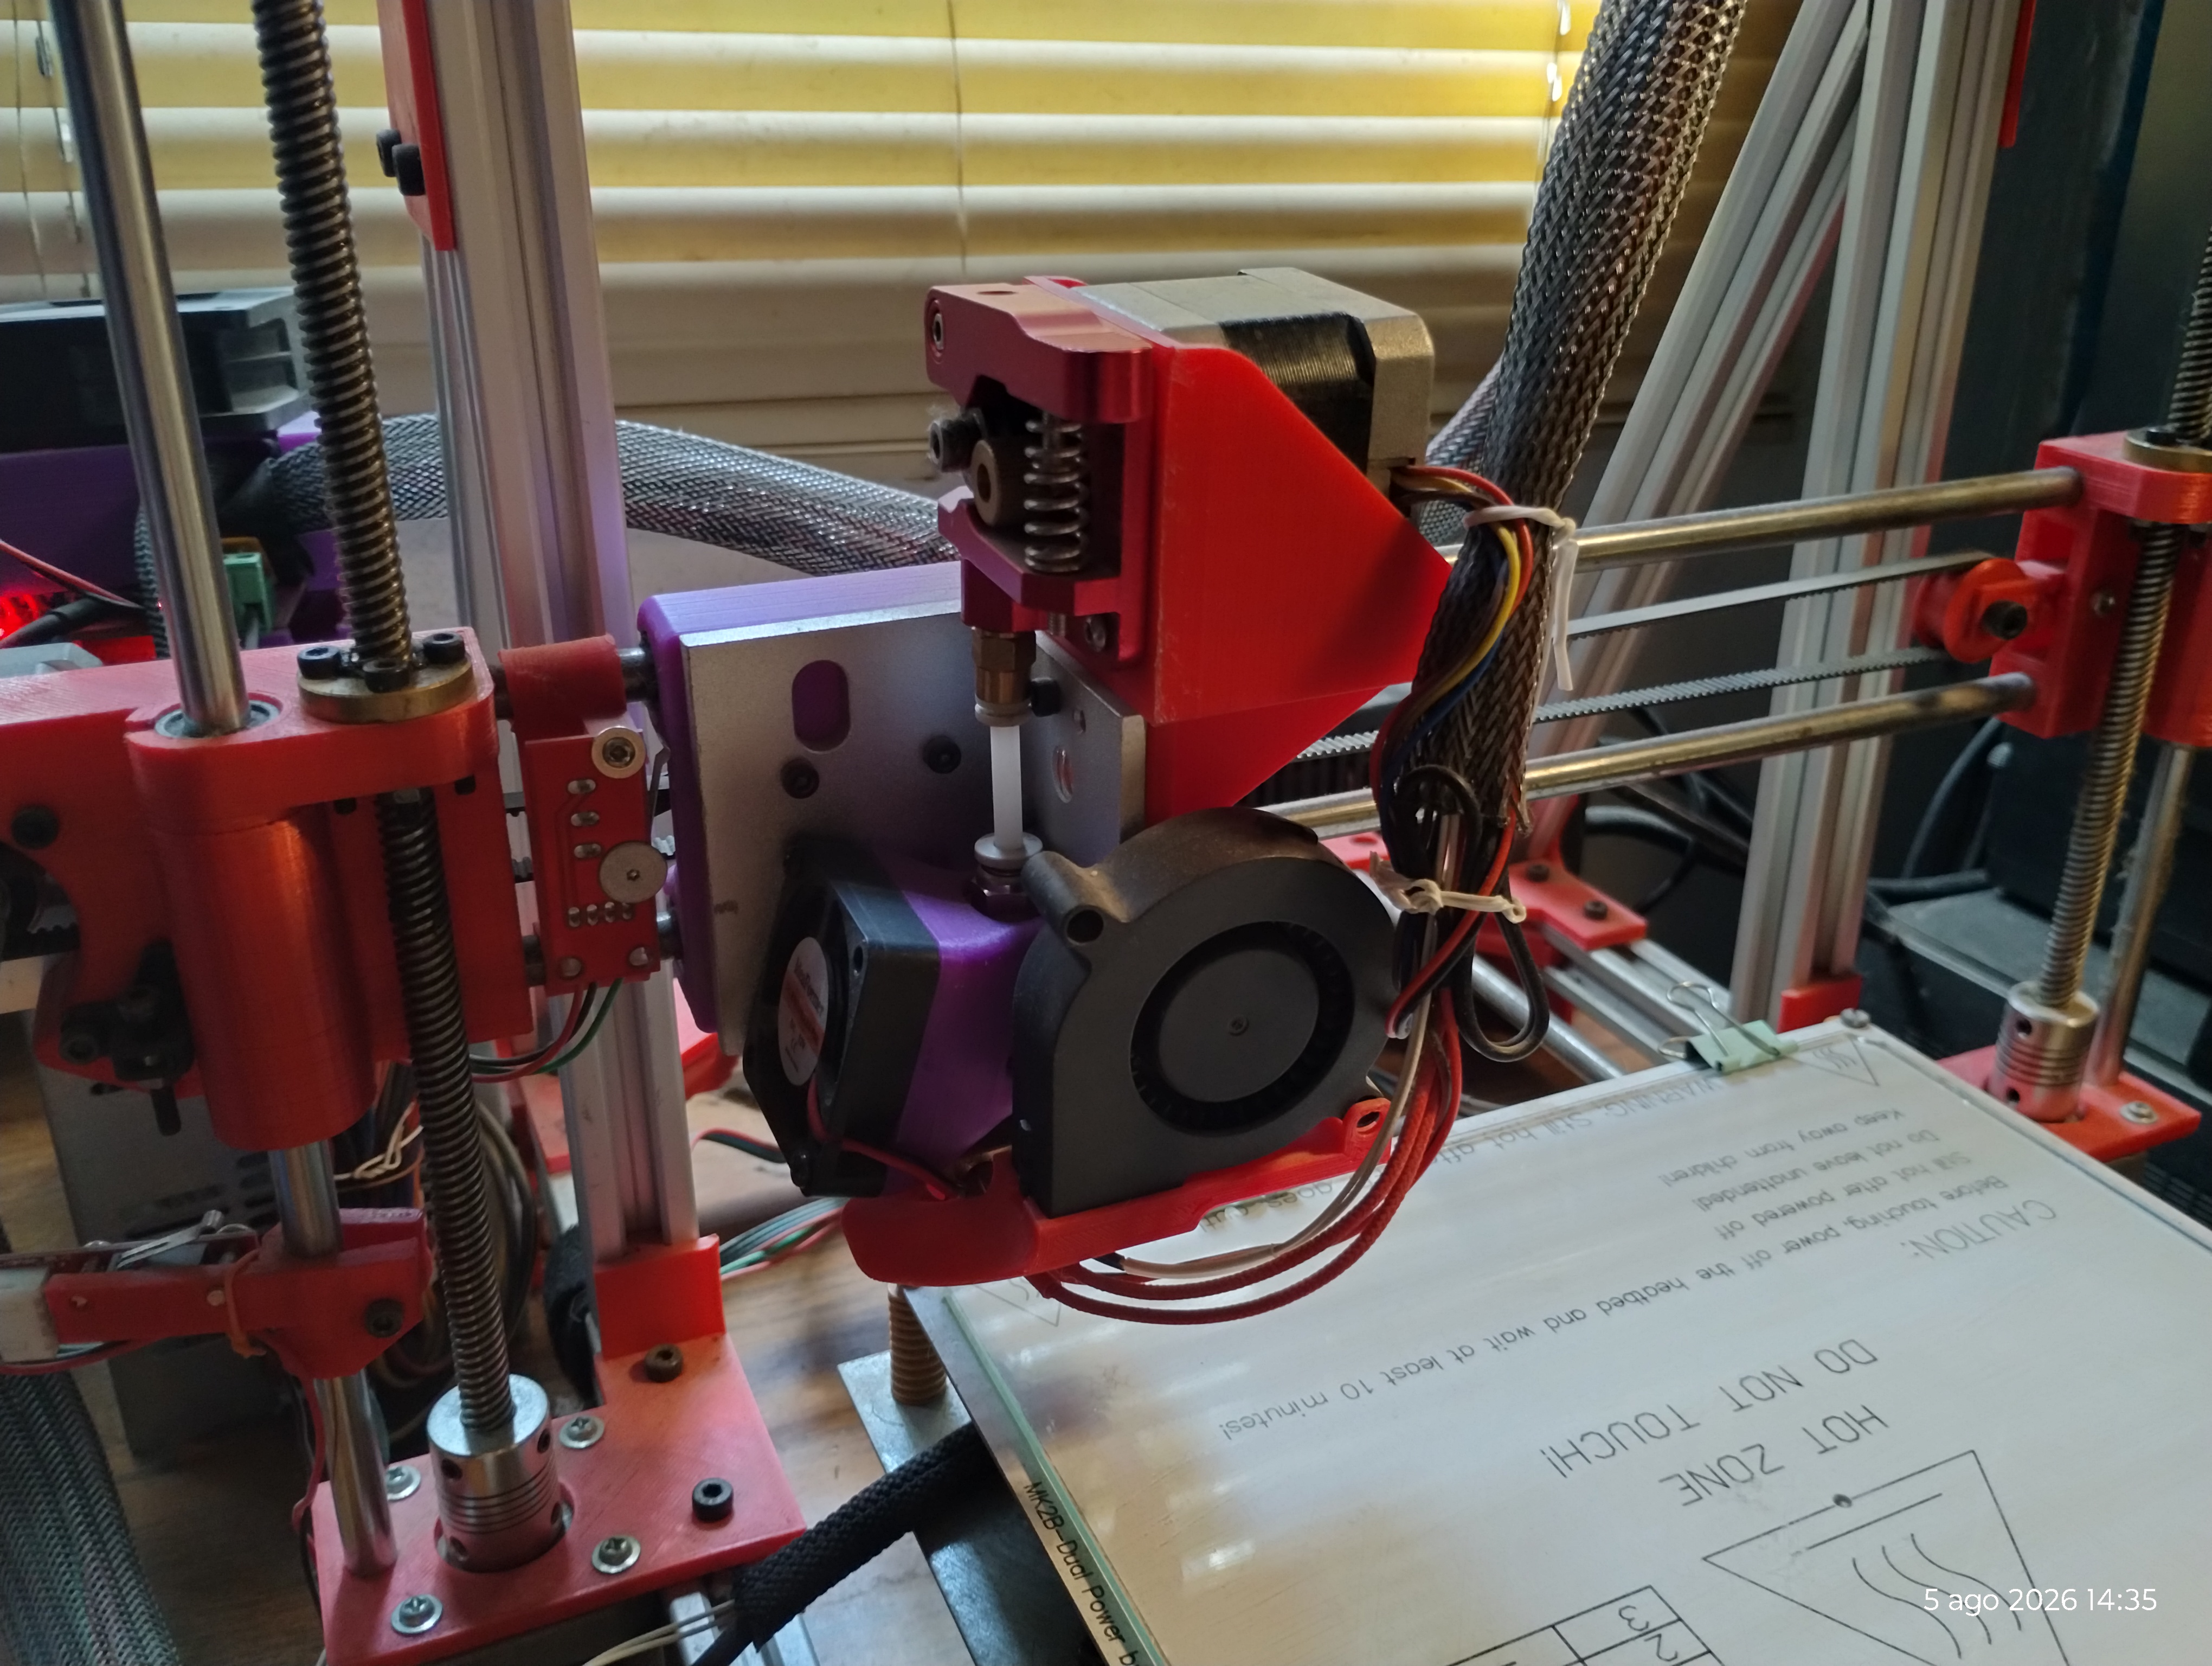
\includegraphics[width=0.5\linewidth]{Extrusor final.jpg}
    \caption{Módulo de extrusión en su configuración final.}
    \label{fig:extrusor_final}
\end{figure}


Las dimensiones generales y la masa del sistema de extrusión se presentan en la Tabla \ref{tab:comparacion_extrusion2}. Para facilitar la comparación, se incluyen los valores correspondientes a la configuración original y a la configuración rediseñada.


\begin{table}[htbp]
    \centering
    \caption{Comparación dimensional y de masa del sistema de extrusión.}
    \label{tab:comparacion_extrusion2}
    \begin{tabular}{lccc}
        \toprule
        \textbf{Característica} & \textbf{Original} & 
        \textbf{Rediseñado} & \textbf{Variación} \\
        \midrule
        Alto          & \qty{18}{\cm} & \qty{14}{\cm} & \qty{-4}{\cm} \\
        Ancho         & \qty{12}{\cm} & \qty{10}{\cm} & \qty{-2}{\cm} \\
        Largo         & \qty{9}{\cm}  & \qty{7}{\cm}  & \qty{-2}{\cm} \\
        Masa total    & \qty{650}{\g} & \qty{493}{\g} & \qty{-157}{\g} \\
        \midrule
        Recorrido Z disponible & \qty{180}{\mm} & \qty{250}{\mm} 
        & \qty{70}{\mm} \\
        \bottomrule
    \end{tabular}
\end{table}

El módulo rediseñado presentó una reducción de \qty{4}{\cm} en altura, 
\qty{2}{\cm} en ancho y \qty{2}{\cm} en largo respecto a la configuración 
original. La masa total se redujo de \qty{650}{\g} a \qty{493}{\g}, lo que 
representa una disminución de \qty{157}{\g}, equivalente al 24.2\% de la masa 
original.

\section{Validación del sistema de movimiento}
\label{sec:validacion_movimiento}

Tras aplicar el procedimiento de calibración descrito en la subsección \ref{sec:calibracion_del_sistema_de_movimiento}, se verificó la correspondencia entre el desplazamiento programado y el desplazamiento real de cada eje. Los resultados obtenidos se presentan en la Tabla \ref{tab:precision_ejes}.


\begin{table}[htbp]
    \centering
    \small
    \caption{Evaluación de la precisión dimensional y error por eje.}
    \label{tab:precision_ejes}
    \begin{tabularx}{\textwidth}{c X X X X}
        \toprule
        \textbf{Eje} & 
        \textbf{Distancia programada} & 
        \textbf{Distancia medida} & 
        \textbf{Error absoluto} & 
        \textbf{Error (\%)} \\
        \midrule
        \(X\) & \qty{100.0}{\mm} & \qty{100.2}{\mm} & \qty{0.2}{\mm} & 0.20\,\% \\
        \(Y\) & \qty{100.0}{\mm} & \qty{99.7}{\mm}  & \qty{0.3}{\mm} & 0.30\,\% \\
        \(Z\) & \qty{100.0}{\mm} & \qty{100.2}{\mm} & \qty{0.2}{\mm} & 0.20\,\% \\
        \bottomrule
    \end{tabularx}
\end{table}

Los tres ejes presentaron errores absolutos inferiores a \qty{0.5}{\mm}, 
lo que corresponde a errores relativos menores al 0.5\%. El eje \(Y\) 
presentó el error más alto (\qty{0.3}{\mm}), mientras que los ejes \(X\) y 
\(Z\) presentaron errores de \qty{0.2}{\mm} cada uno.

\subsection{Validación del sistema térmico}
\label{sec:validacion_termica}
Tras aplicar el procedimiento de calibración descrito en la 
sección~\ref{sec:calibracion_termica}, se obtuvieron las constantes de 
control PID para el hotend y para la cama calefactada. La 
Tabla~\ref{tab:pid_final} presenta los valores finales incorporados al 
firmware.

% ============================================================
% CÓMO OBTENER LAS CONSTANTES PID:
% 
% Opción A (desde la impresora):
%   1. Conectar la impresora a Pronterface, OctoPrint o similar.
%   2. Enviar el comando M503 (reporta la configuración actual).
%   3. Buscar las líneas:
%      M301 P... I... D...   (para el hotend)
%      M304 P... I... D...   (para la cama calefactada)
%   4. Anotar los valores de P, I, D.
%
% Opción B (ejecutar autotune de nuevo):
%   1. Enviar M303 E0 S200 C8   (hotend a 200°C, 8 ciclos)
%   2. Enviar M303 E-1 S60 C8   (cama a 60°C, 8 ciclos)
%   3. Marlin reporta los valores al final de cada autotune.
%   4. Anotar los valores y guardarlos con M500.
% ============================================================


\begin{table}[htbp]
    \centering
    \caption{Constantes PID obtenidas para el hotend y la cama calefactada.}
    \label{tab:pid_final}
    \begin{tabular}{lccc}
        \toprule
        \textbf{Componente} & \textbf{$K_p$} & 
        \textbf{$K_i$} & \textbf{$K_d$} \\
        \midrule
        Hotend        & [dato] & [dato] & [dato] \\
        Cama calefactada & [dato] & [dato] & [dato] \\
        \bottomrule
    \end{tabular}
\end{table}

% ============================================================
% CÓMO OBTENER LAS TABLAS DE TEMPERATURA PROGRAMADA VS ALCANZADA:
%
% Estas pruebas verifican la precisión del control en estado estable.
% 
% Procedimiento para el hotend:
%   1. Enviar M104 S200  (o usar el menú de la impresora para fijar 200°C)
%   2. Esperar 2 minutos a que se estabilice.
%   3. Leer la temperatura actual desde la pantalla o con M105.
%   4. Anotar el valor.
%   5. Repetir con 210°C y 220°C.
%
% Procedimiento para la cama:
%   Igual, pero con M140 S60, luego S70 y S80.
%   La cama tarda más en estabilizarse, esperar 5 minutos.
%
% Toma al menos 3 lecturas por temperatura y promedia.
% ============================================================

La Tabla~\ref{tab:temp_hotend} presenta las temperaturas programadas y 
alcanzadas en el hotend para tres valores de referencia, mientras que la 
Tabla~\ref{tab:temp_cama} presenta los resultados equivalentes para la cama 
calefactada.

\begin{table}[htbp]
    \centering
    \caption{Temperatura programada frente a alcanzada en el hotend.}
    \label{tab:temp_hotend}
    \begin{tabular}{ccc}
        \toprule
        \textbf{Prueba / Ensayo} & \textbf{Temp. Programada} & \textbf{Temp. Alcanzada} \\
        \midrule
        1 & \qty{200}{\celsius} & \qty{200.2}{\celsius} \\
        2 & \qty{210}{\celsius} & \qty{210.1}{\celsius} \\
        3 & \qty{220}{\celsius} & \qty{220.0}{\celsius} \\
        \bottomrule
    \end{tabular}
\end{table}

\begin{table}[htbp]
    \centering
    \caption{Temperatura programada frente a alcanzada en la cama caliente.}
    \label{tab:temp_cama}
    \begin{tabular}{ccc}
        \toprule
        \textbf{Prueba / Ensayo} & \textbf{Temp. Programada} & \textbf{Temp. Alcanzada} \\
        \midrule
        1 & \qty{60}{\celsius} & \qty{59.8}{\celsius} \\
        2 & \qty{70}{\celsius} & \qty{70.1}{\celsius} \\
        3 & \qty{80}{\celsius} & \qty{80.2}{\celsius} \\
        \bottomrule
    \end{tabular}
\end{table}

% ============================================================
% CÓMO OBTENER LA GRÁFICA DE TEMPERATURA VS TIEMPO:
%
% Esta prueba mide la estabilidad dinámica durante la impresión real.
%
% Método 1 (con Pronterface / OctoPrint):
%   1. Cargar una pieza de prueba (ej. cubo de 20x20x20 mm).
%   2. En Pronterface: pestaña "Temperature Graph" o 
%      en OctoPrint: pestaña "Temperature".
%   3. Iniciar la impresión.
%   4. La gráfica se genera automáticamente.
%   5. Capturar la pantalla después de 10-15 min de impresión.
%
% Método 2 (registro manual):
%   1. Durante la impresión, enviar M105 cada 30 segundos.
%   2. Anotar: tiempo, temperatura actual, temperatura objetivo.
%   3. Repetir durante 10-15 minutos.
%   4. Graficar en Excel o Python (tiempo vs temperatura).
%
% Análisis a reportar:
%   - Variación máxima (temp. máx - temp. mín).
%   - Desviación estándar.
%   - Si la variación es ≤ ±2°C, el control es estable.
% ============================================================

La Figura~\ref{fig:grafica_temperatura} presenta el comportamiento de la temperatura del hotend durante una impresión de prueba de 15 minutos. El registro se realizó con el software [COMPLETAR: Pronterface/OctoPrint/Otro].

\begin{comment}
\begin{figure}[H]
    \centering
    \includegraphics[width=0.8\linewidth]{Grafica_temperatura_hotend.png}
    \caption{Respuesta térmica del hotend durante la impresión.}
    \label{fig:grafica_temperatura}
\end{figure}
\end{comment}


Durante el período registrado, la temperatura del hotend se mantuvo dentro de un rango de \qty{\pm 0000}{\celsius} respecto a la temperatura de referencia, con una desviación estándar de \qty{0000}{\celsius}. Este resultado indica que el lazo de control mantiene la temperatura estable incluso ante las demandas dinámicas del proceso de extrusión.

% ============================================================
% CÓMO OBTENER EL TIEMPO DE CALENTAMIENTO:
%
% Procedimiento:
%   1. Con la impresora a temperatura ambiente (registrar la temp. inicial).
%   2. Enviar M104 S200 y arrancar un cronómetro.
%   3. Detener el cronómetro cuando la temperatura alcance 200°C.
%   4. Anotar el tiempo.
%   5. Repetir con la cama: M140 S60, medir tiempo hasta 60°C.
% ============================================================

La Tabla~\ref{tab:tiempo_calentamiento} presenta el tiempo requerido por 
cada componente para alcanzar su temperatura de operación desde temperatura 
ambiente, así como la variación en estado estable una vez alcanzada la 
referencia.

\begin{comment}
    

\begin{table}[htbp]
    \centering
    \caption{Tiempo de calentamiento y variación en estado estable.}
    \label{tab:tiempo_calentamiento}
    \begin{tabular}{lcc}
        \toprule
        \textbf{Componente} & \textbf{Tiempo de calentamiento} & 
        \textbf{Variación en estado estable} \\
        \midrule
        Hotend        & [dato] s & \(\pm\)[dato]\celsius \\
        Cama calefactada & [dato] s & \(\pm\)[dato]\celsius \\
        \bottomrule
    \end{tabular}
\end{table}


\begin{comment}
    

     \begin{table}[htbp]
    \centering
    \caption{Tabla de tiempo de calentamiento y variación en estado estable para hotend y cama.}
    \label{tab:temp_cama3}
    \begin{tabular}{ccc}
        \toprule
        \textbf{Prueba / Ensayo} & \textbf{Temp. Programada} & \textbf{Temp. Alcanzada} \\
        \midrule
        1 & \qty{60}{\celsius} & \qty{59.8}{\celsius} \\
        2 & \qty{70}{\celsius} & \qty{70.1}{\celsius} \\
        3 & \qty{80}{\celsius} & \qty{80.2}{\celsius} \\
        \bottomrule
    \end{tabular}
\end{table}

\end{comment}   


\section{Validación del sistema de extrusión}
\label{sec:validacion_extrusion}

Tras aplicar el procedimiento de calibración descrito en la 
sección~\ref{sec:calibracion_extrusor}, se verificó la cantidad de filamento 
suministrada por el mecanismo de alimentación. La 
Tabla~\ref{tab:calibracion_extrusor} presenta los resultados de la prueba de 
verificación.

% ============================================================
% CÓMO OBTENER LOS DATOS:
%
% Esta prueba ya la hiciste durante la calibración (sección 6.6.3).
% Solo necesitas recuperar los valores que anotaste:
%   - Longitud programada: 100 mm
%   - Longitud medida: [el valor real que mediste]
%   - Error absoluto: [programada - medida]
%   - Error (%): [(error absoluto / programada) × 100]
%   - Pasos/mm finales: [el valor que quedó en el firmware]
% ============================================================

\begin{table}[htbp]
    \centering
    \caption{Verificación de la calibración del extrusor.}
    \label{tab:calibracion_extrusor}
    \begin{tabular}{lcc}
        \toprule
        \textbf{Parámetro} & \textbf{Valor} \\
        \midrule
        Longitud programada          & \qty{100}{\mm} \\
        Longitud medida              & [dato] \unit{\mm} \\
        Error absoluto               & [dato] \unit{\mm} \\
        Error relativo               & [dato]\,\% \\
        Pasos por milímetro finales  & [dato] \\
        \bottomrule
    \end{tabular}
\end{table}

% ============================================================
% CÓMO VERIFICAR LA AUSENCIA DE DEFORMACIÓN DEL SOPORTE:
%
% Procedimiento:
%   1. Imprimir una pieza de prueba de al menos 30 minutos de duración.
%   2. Al terminar, revisar visualmente el soporte del motor y la base 
%      de aluminio.
%   3. Verificar que no haya deformación, decoloración ni 
%      desprendimiento.
%   4. Opcional: medir la temperatura del soporte con termopar 
%      después de 30 min de impresión.
%
% Si el soporte no presentó deformación, indícalo. Si presentó 
% alguna, descríbela.
% ============================================================

Adicionalmente, se monitoreó el estado del soporte del motor y de la base 
estructural durante la fabricación de las piezas del proyecto (algunas de las 
cuales requirieron varias horas de impresión). A diferencia de la primera 
iteración, en la que el soporte de PLA se deformó por la transferencia de 
calor, en esta configuración final no se observó deformación, decoloración ni 
pérdida de rigidez en los componentes poliméricos. Esto confirma que la 
separación térmica proporcionada por la base de aluminio y la ventilación 
forzada cumplen su función durante la operación normal del equipo.

\section{Validación del sistema de enfriamiento}
\label{sec:validacion_enfriamiento}

El sistema de enfriamiento del hotend tiene como propósito evacuar el calor residual del disipador para evitar que se propague hacia la zona fría del hotend y provoque el ablandamiento prematuro del filamento (\textit{heat creep}). Para evaluar la efectividad del sistema desarrollado, se realizaron mediciones de temperatura en el disipador del hotend bajo distintas condiciones de disipación.

Para las mediciones se utilizó un termopar tipo K colocado en la superficie 
externa del disipador del hotend, a media altura. La Figura~\ref{fig:posicion_sensor} muestra la ubicación exacta del sensor. En todas las pruebas se mantuvo el mismo punto de medición y se esperó un tiempo de 5 minutos a que la temperatura se estabilizara antes de registrar cada lectura. La temperatura del bloque calefactor se mantuvo en \qty{200}{\celsius} como referencia en todos los casos.

La Tabla~\ref{tab:disipacion} presenta las temperaturas registradas en el disipador bajo cada condición evaluada.

\begin{table}[htbp]
    \centering
    \caption{Temperaturas registradas en el disipador del hotend bajo distintas condiciones de disipación.}
    \label{tab:disipacion}
    \begin{tabular}{lcc}
        \toprule
        \textbf{Condición} & \textbf{Temperatura en disipador} & 
        \textbf{Temperatura en bloque calefactor} \\
        \midrule
        Sin disipador ni ventilador & \qty{71}{\celsius} & \qty{200}{\celsius} \\
        Con base de aluminio, sin ventilador & \qty{41}{\celsius} & \qty{200}{\celsius} \\
        Con base de aluminio y ventilador & \qty{47}{\celsius} & \qty{200}{\celsius} \\
        \bottomrule
    \end{tabular}
\end{table}

La incorporación de la base estructural de aluminio redujo la temperatura 
del disipador de \qty{71}{\celsius} a \qty{41}{\celsius}, lo que representa 
una disminución de \qty{30}{\celsius}, equivalente a una reducción del 
42.25\% respecto a la condición sin disipación. La adición del ventilador 
redujo la temperatura en \qty{11111}{\celsius} adicionales, alcanzando un valor final de \qty{11111}{\celsius} y una reducción total del 99\% respecto a la condición inicial.


\begin{figure}[H]
    \centering
    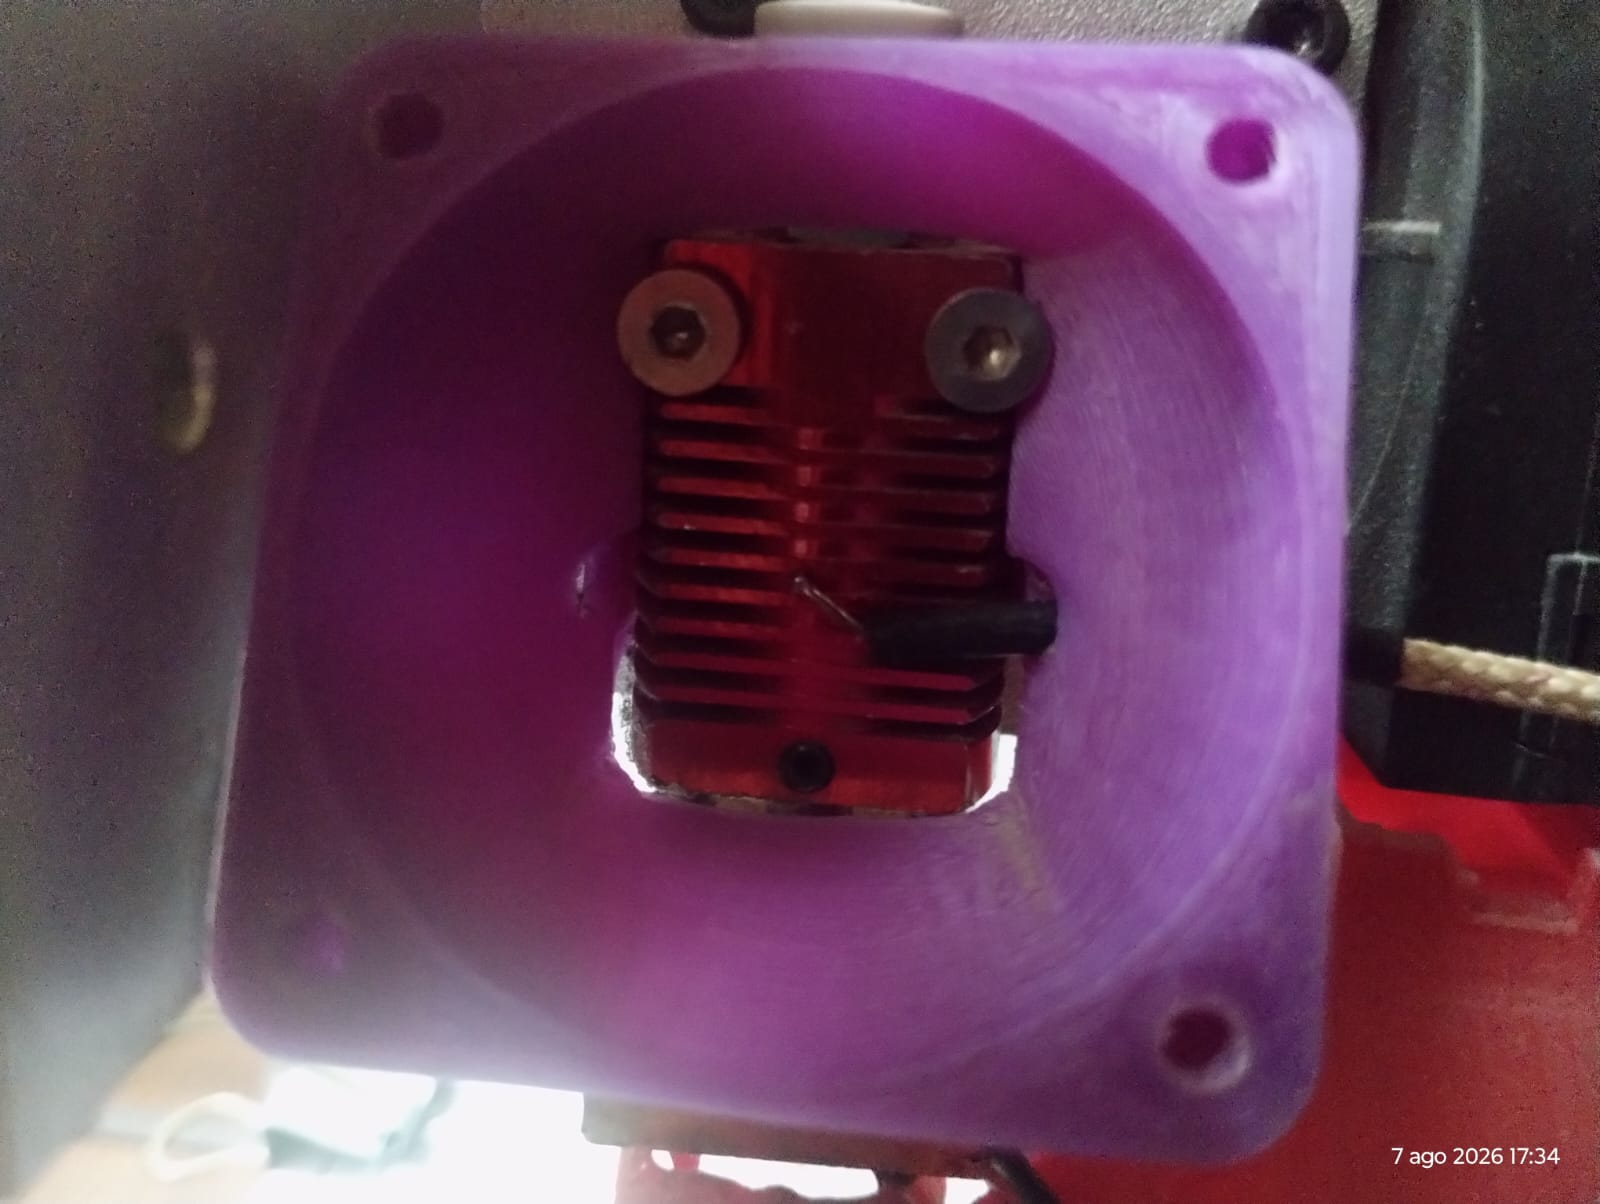
\includegraphics[width=0.5\linewidth]{Evidencia_posicion_sensor.jpeg}
    \caption{Evidencia posicionamiento de sensor de pruebas}
    \label{fig:posicion_sensor}
\end{figure}

\section{Evaluación de calidad de impresión}

\subsection{Precisión dimensional}

Evaluando la precisión del equipo conseguido se llegaron a los valores mostrados en la Tabla~\ref{tab:cubos_calibracion}. Donde estan enlistadas las dimensiones de cubos de prueba. Las dimensiones se midieron con un vernier marca Truper con resolución de \qty{0.02}{\mm}. 

\begin{table}[htbp]
    \centering
    \caption{Dimensiones y errores de los cubos de calibración.}
    \label{tab:cubos_calibracion}
    \begin{tabular}{lcccc}
        \toprule
        \textbf{Eje} & \textbf{Dimensión CAD} & \textbf{Dimensión medida} & \textbf{Error (mm)} & \textbf{Error (\%)} \\
        \midrule
        \(X\) & \qty{20.00}{\mm} & \qty{20.30}{\mm} & \qty{+0.30}{\mm} & +1.50\% \\
        \(Y\) & \qty{20.00}{\mm} & \qty{20.10}{\mm} & \qty{+0.10}{\mm} & +0.50\% \\
        \(Z\) & \qty{20.00}{\mm} & \qty{20.14}{\mm} & \qty{+0.14}{\mm} & +0.70\% \\
        \bottomrule
    \end{tabular}
\end{table}


\subsection{Pruebas geométricas}
\label{subsec:pruebas_geometricas}

Se realizaron pruebas geométricas estándar para evaluar la capacidad del 
sistema de imprimir geometrías complejas. Las pruebas incluyeron overhang, 
stringing y una torre de temperatura. Las Figuras~\ref{fig:overhang} a \ref{fig:torre_temperatura} muestran las piezas obtenidas.

\begin{figure}[H]
    \centering
    \begin{subfigure}[b]{0.45\linewidth}
        \centering
        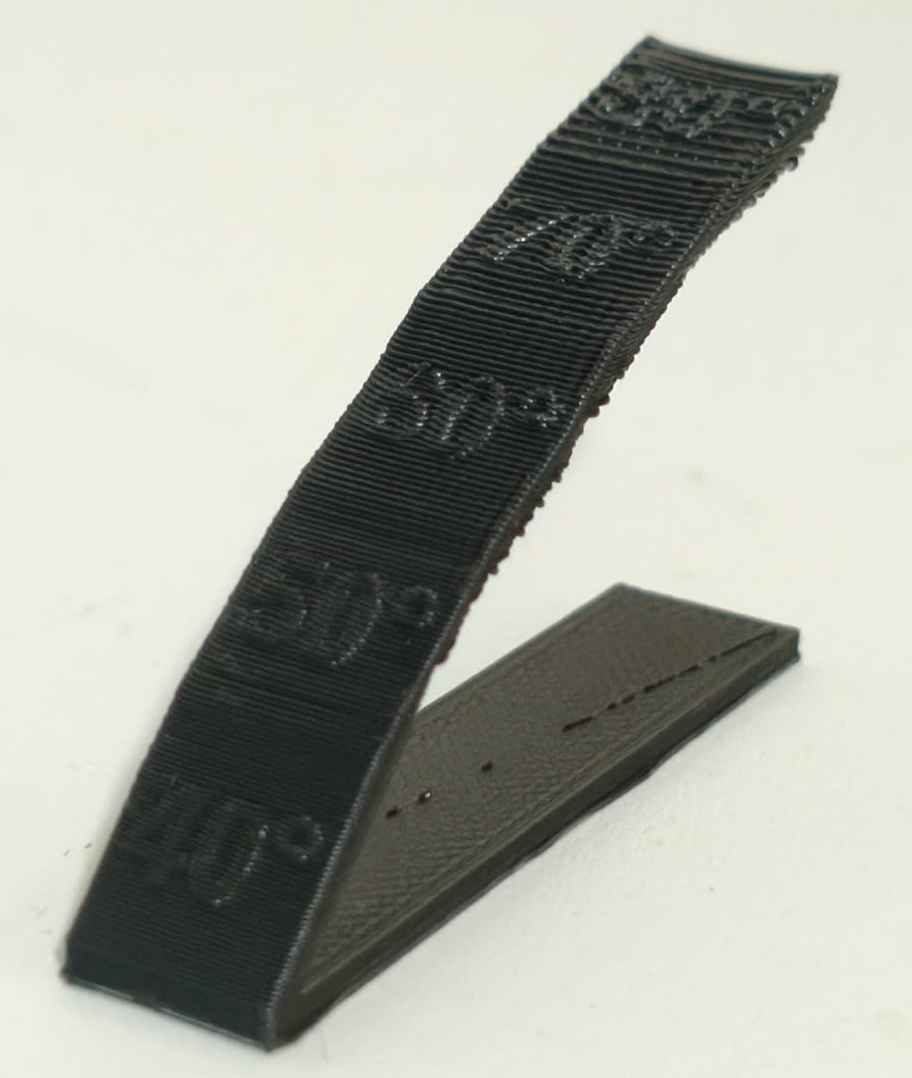
\includegraphics[width=\linewidth]{overhang.jpg}
        \caption{Prueba de overhang.}
        \label{fig:overhang}
    \end{subfigure}
    \hfill
    \begin{subfigure}[b]{0.4\linewidth}
        \centering
        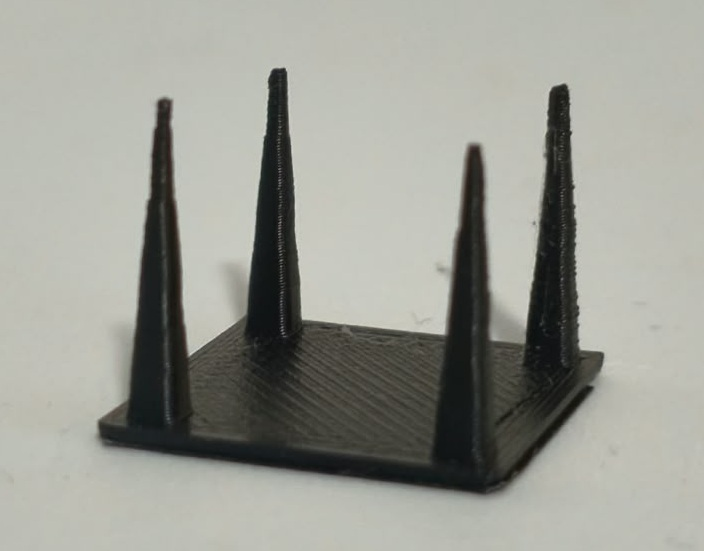
\includegraphics[width=\linewidth]{stringing.jpg}
        \caption{Prueba de stringing.}
        \label{fig:stringing}
    \end{subfigure}
    \caption{Pruebas geométricas: overhang (izquierda) y stringing (derecha).}
    \label{fig:pruebas_overhang_stringing}
\end{figure}

\begin{figure}[H]
    \centering
    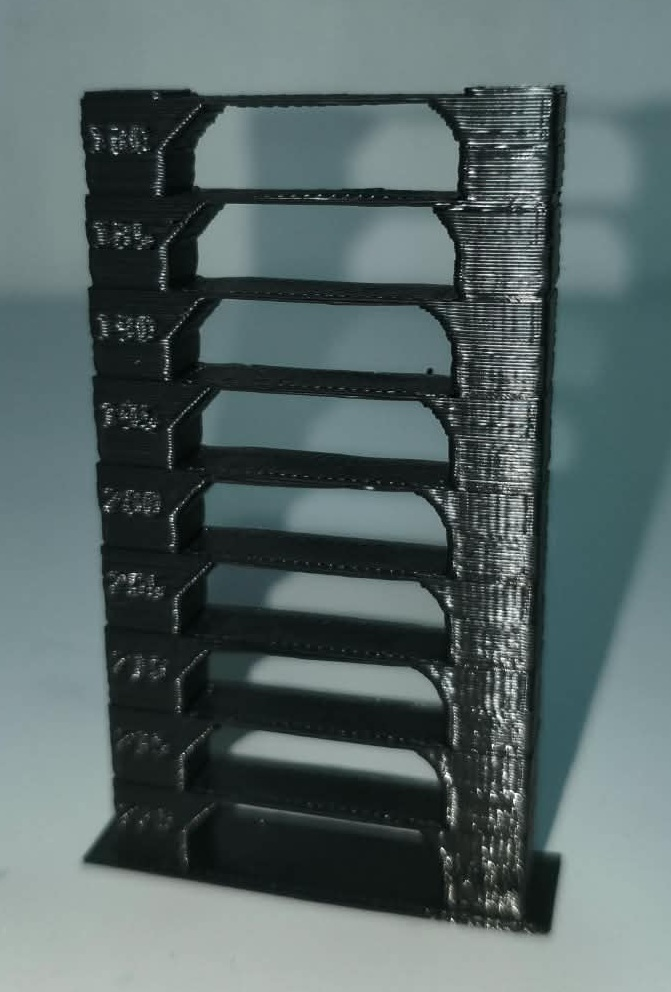
\includegraphics[width=0.5\linewidth]{torre_temperatura.jpg}
    \caption{Torre de temperatura.}
    \label{fig:torre_temperatura}
\end{figure}

\textbf{Overhang:} La pieza de prueba consistió en una geometría escalonada que varió desde \ang{40} hasta \ang{80} en incrementos de \ang{10}. Hasta \ang{70} la pieza no presentó deflexión apreciable. A partir de ese ángulo se observó un incremento en la visibilidad de las líneas de capa, que se 
acentuó a \ang{80}. No obstante, en ningún caso se produjo el colapso de la estructura, por lo que el sistema mantuvo la continuidad de la impresión en toda la pieza.

\textbf{Stringing:} La pieza de prueba consistió en cuatro torres separadas. No se observó formación significativa de hilos entre las torres; únicamente se apreciaron un par de filamentos muy finos que no resultaron visibles en la fotografía. Las torres conservaron su forma y sus dimensiones sin presentar defectos apreciables.

\textbf{Torre de temperatura:} La torre se imprimió en un rango de \qty{220}{\celsius} en la base hasta \qty{180}{\celsius} en la parte superior, con decrementos de \qty{5}{\celsius} por escalón. A simple vista, todos los escalones presentaron una impresión satisfactoria. Sin embargo, al inspeccionar la pieza a contraluz se observaron diferencias notables entre los escalones.

Los escalones correspondientes al rango de \qty{210}{\celsius} a 
\qty{220}{\celsius} presentaron translucidez, lo que permitió observar a través de la pieza. Los escalones inferiores, correspondientes al rango de \qty{180}{\celsius} a \qty{190}{\celsius}, mostraron ligeros defectos superficiales. El escalón correspondiente a \qty{205}{\celsius} presentó la mejor combinación de acabado superficial y uniformidad, por lo que este valor se adoptó como temperatura de referencia para las impresiones posteriores.

\subsection{Problemas de impresión presentados y soluciones}
\label{subsec:problemas_soluciones}

A lo largo del desarrollo de las pruebas de impresión se presentaron diversas 
problemáticas que requirieron ajustes iterativos. Dado que las pruebas se 
realizaron en distintas etapas del proyecto y con diferentes materiales, los 
problemas y sus soluciones se describen a continuación de forma cronológica.

\textbf{Ajuste inicial y evolución de la calidad:} Durante las primeras 
fases de calibración, se imprimieron múltiples cubos de prueba para afinar 
los parámetros del laminador. En la Figura~\ref{fig:evolucion_cubos} se 
observa una comparación entre dos cubos impresos consecutivamente con 
configuraciones distintas, donde se aprecia una mejora sustancial en la 
uniformidad de las paredes, la definición de las esquinas y la precisión 
dimensional.

\begin{figure}[h]
    \centering
    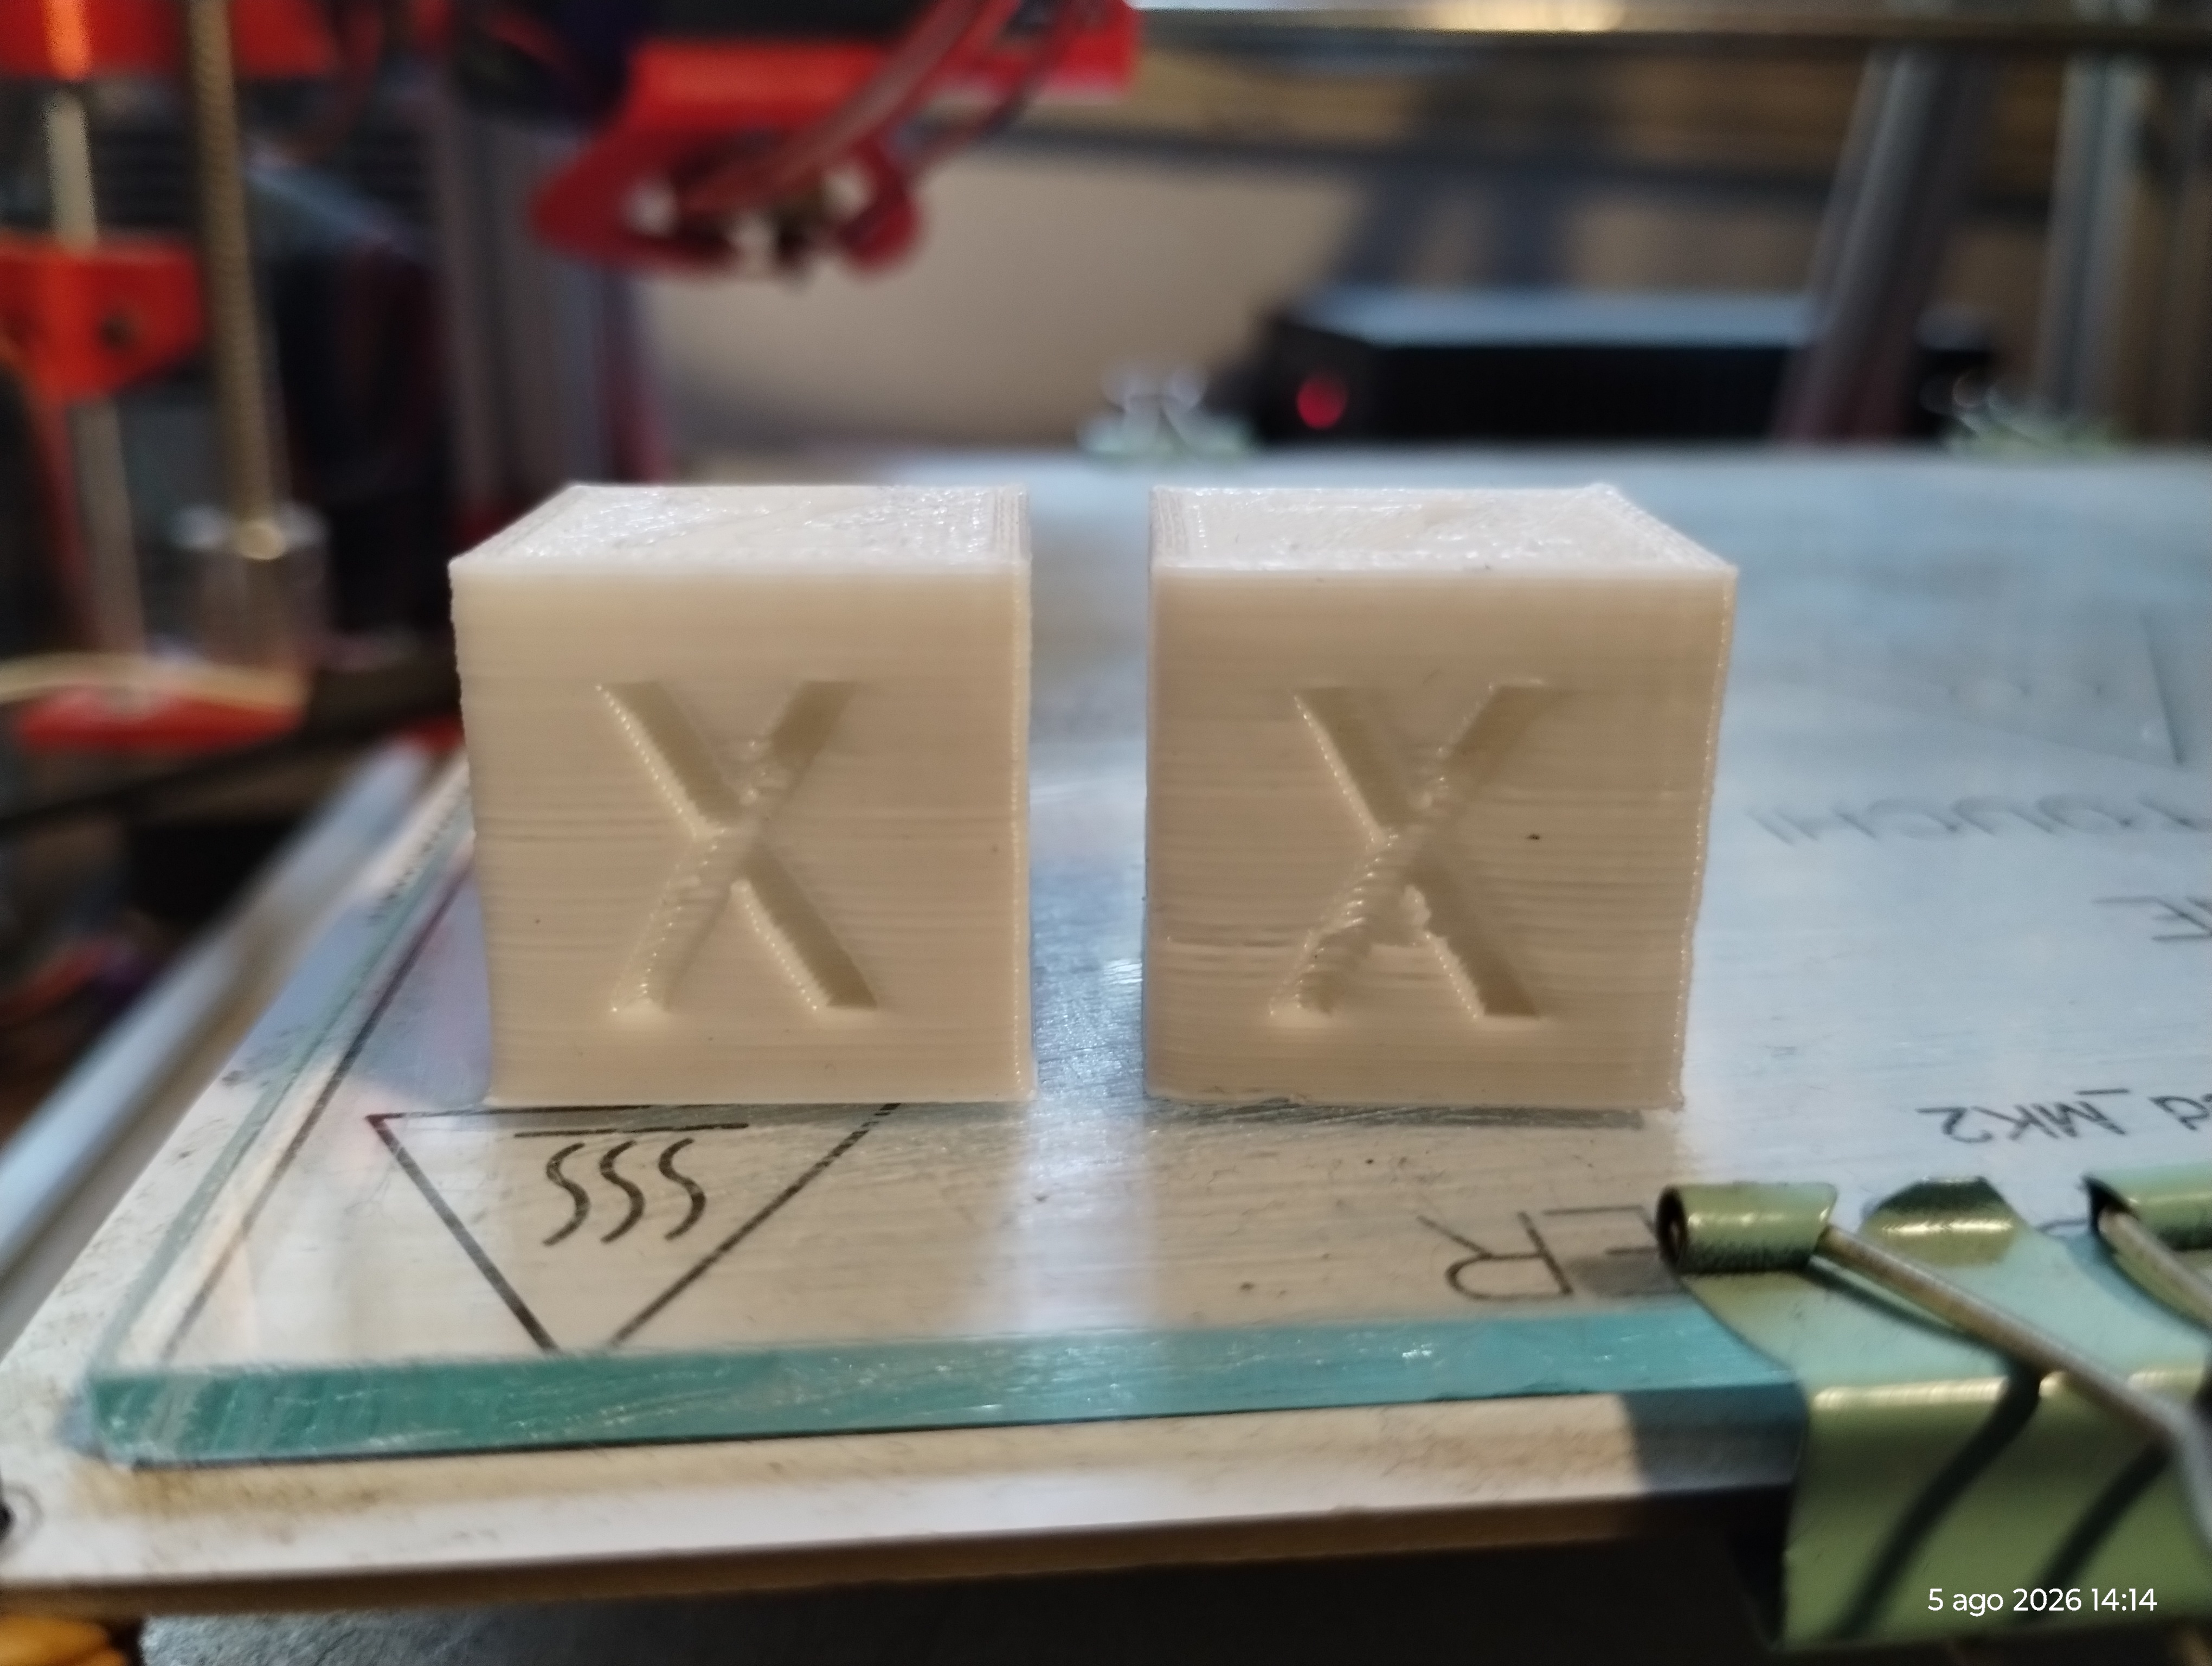
\includegraphics[width=0.5\linewidth]{comparacion calidad.jpg}
    \caption{Comparación entre dos cubos de calibración impresos con diferentes parámetros de configuración.}
    \label{fig:evolucion_cubos}
\end{figure}

\textbf{Diagnóstico de humedad en el filamento:} Tras un periodo de 
impresiones exitosas, la calidad de las piezas comenzó a deteriorarse 
repentinamente. Se verificó que los parámetros del software no se habían 
modificado y que la impresora no presentaba fallas mecánicas (como 
atascamientos o pérdida de pasos). Los síntomas observados en las piezas 
fueron una mayor fragilidad y un acabado superficial inusualmente brillante. 
Tras consultar literatura técnica y foros especializados, se identificó que 
estos síntomas eran característicos de la humedad absorbida por el filamento 
de PLA.

Para comprobar esta hipótesis, se realizó una prueba de control sustituyendo 
el carrete por un filamento nuevo de otra marca. Las impresiones mejoraron 
significativamente desde la primera prueba, lo que confirmó que el problema 
no era mecánico ni de configuración, sino que el filamento anterior había 
absorbido humedad del ambiente. No obstante, el nuevo material requirió un 
ajuste fino en los parámetros del laminador para alcanzar la calidad óptima, 
lo que evidenció que cada marca de filamento posee características propias.

\textbf{Solución aplicada:} Al desconocer inicialmente las recomendaciones de 
almacenamiento del PLA, el carrete había permanecido montado en la impresora 
dentro de una habitación, expuesto a la humedad ambiental. 
Para solucionarlo, 
se implementó un método de secado utilizando la cama calefactada a 
\qty{50}{\celsius} durante 3 horas. Posteriormente, el mismo carrete se volvió 
a montar para imprimir una pieza de prueba, y se observó una recuperación 
notable en la calidad: desaparecieron las superficies irregulares y la fragilidad de la pieza disminuyó. A partir de este hallazgo, se estableció un procedimiento de almacenamiento de los carretes de filamento en bolsas herméticas con desecante.

\textbf{Diferencias entre marcas de filamento:} El uso de carretes de 
distintas marcas durante el proyecto evidenció que no todos los filamentos 
de PLA se comportan de la misma manera. Se observó que el filamento de la 
marca [COMPLETAR] requería una temperatura de [dato]\,\(^\circ\)C, mientras 
que el de la marca [COMPLETAR] presentaba mejores resultados a 
[dato]\,\(^\circ\)C. Esta variación se atribuye a diferencias en la 
composición química del polímero, los aditivos colorantes y el diámetro real 
del filamento.


\section{Evaluación económica}
La evaluación económica tiene como propósito determinar la viabilidad del sistema desarrollado frente a alternativas comerciales equivalentes. Para ello, se analizan dos aspectos: el costo de fabricación del equipo y la comparación con impresoras comerciales de gama similar. Los precios se expresan en pesos mexicanos (MXN) y corresponden a cotizaciones obtenidas durante el desarrollo del proyecto. No se incluye el costo de mano de obra, ya que el ensamblaje y la calibración fueron realizados por los autores como parte del trabajo académico. 

\subsection{Costo de fabricación}
En la Tabla~\ref{tab:costo_fabricacion} se presenta el desglose de los componentes utilizados en la fabricación e integración de la impresora. Se incluyen tanto los elementos electrónicos como los mecánicos y auxiliares.

\begin{table}[H]
    \centering
    \small
    \caption{Costo de fabricación de la impresora custom.}
    \label{tab:costo_fabricacion}
    \begin{tabular}{lccc}
        \toprule
        \textbf{Componente} & \textbf{Cantidad} & \textbf{Costo unitario} & \textbf{Costo total} \\
        \midrule
        Arduino Mega                    & 1 pza.            & \$189.00 & \$189.00 \\
        Placa RAMPS 1.4                 & 1 pza.            & \$94.00  & \$94.00  \\
        Motores NEMA 17                 & 4 pzas.           & \$32.00  & \$128.00 \\
        Cables para motor               & 4 pzas.           & \$27.25  & \$109.00 \\
        Hotend Ender Creality CR-10     & 1 pza.            & \$138.00 & \$138.00 \\
        Cama calefactada                   & 1 pza.            & \$274.00 & \$274.00 \\
        Fuente de poder                 & 1 pza.            & \$299.00 & \$299.00 \\
        Drivers A4988 con disipador     & 4 pzas.           & \$30.50  & \$122.00 \\
        Ventilador \qty{12}{\V}, \qty{40}{\mm} & 2 pzas.   & \$29.50  & \$59.00  \\
        Extrusor Ender Creality CR-10S  & 1 pza.            & \$106.00 & \$106.00 \\
        Resortes para cama              & 4 pzas.           & \$21.00  & \$84.00  \\
        Tubo de teflón PTFE translúcido & 2 m               & \$47.00  & \$94.00  \\
        Microswitch endstop             & 3 pzas.           & \$64.67  & \$194.00 \\
        Banda dentada GT2               & 2 pzas.           & \$64.50  & \$129.00 \\
        Polea dentada GT2 20T           & 2 pzas.           & \$37.00  & \$74.00  \\
        Termistor NTC 100K              & 2 pzas.           & \$38.00  & \$76.00  \\
        Tubo termocontráctil            & 1 lote            & \$30.00  & \$30.00  \\
        Lámina galvanizada              & 1 pza.            & \$100.00 & \$100.00 \\
        Rodamientos lineales            & 8 pzas.           & \$9.00   & \$72.00  \\
        Rodamientos                     & 3 pzas.           & \$10.00  & \$30.00  \\
        Tuerca T M4                     & 50 pzas.          & \$2.70   & \$135.00 \\
        Husillo                         & 2 pzas.           & \$125.00 & \$250.00 \\
        Coples                          & 2 pzas.           & \$70.00  & \$140.00 \\
        Varilla lisa                    & 4 pzas.           & \$53.25  & \$213.00 \\
        Vidrio                          & 1 pza.            & \$50.00  & \$50.00  \\
        Perfil de aluminio extruido     & 6 m               & \$166.67 & \$1000.00 \\
        \midrule
        \textbf{Costo total}            &                   &          & \textbf{\$4189.00} \\
        \bottomrule
    \end{tabular}
\end{table}

El costo total de fabricación de la impresora custom fue de \$4189 MXN. Este valor incluye únicamente los componentes listados; no se incluyen costos de mano de obra, envío ni herramientas.

\subsection{Comparación con alternativas comerciales}
Se seleccionaron dos impresoras comerciales de gama similar: Creality Ender 3 V3\cite{creality_ender3v3} y Bambu Lab A1 \cite{bambu_a1}. Ambas ofrecen volúmenes de impresión comparables y están orientadas a usuarios no especializados. La Tabla~\ref{tab:comparacion_de_especificaciones} resume las especificaciones técnicas más relevantes, mientras que la Tabla~\ref{tab:comparacion_costo_comercial} compara los costos totales.

\begin{table}[H]
    \centering
    \caption{Comparación de especificaciones técnicas.}
    \label{tab:comparacion_de_especificaciones}
    \footnotesize
    \begin{tabularx}{\textwidth}{>{\centering\arraybackslash}X >{\centering\arraybackslash}X >{\centering\arraybackslash}X >{\centering\arraybackslash}X}
        \toprule
        \textbf{Especificación} & \textbf{Ender 3 V3} & \textbf{Bambu Lab A1} & \textbf{Impresora Custom} \\
        \midrule
        Volumen de impresión (mm) & 220$\times$220$\times$250 & 256$\times$256$\times$256 & 200$\times$200$\times$180 \\
        Dimensiones del equipo (mm) & 349$\times$364$\times$490 & 385$\times$430$\times$410 & 470$\times$520$\times$570 \\
        Peso bruto (kg) & 7.12 & 8.3 & 7.2 \\
        Extrusor directo & $\checkmark$ & $\checkmark$ & $\checkmark$ \\
        Materiales soportados & PLA, PETG, TPU & PLA, PETG, TPU, PVA & PLA \\
        Superficie de impresión & Lámina de acero con recubrimiento PC & Acero + aluminio extruido & Vidrio + aluminio extruido \\
        Pantalla & 3.2" color con perilla & 3.5" táctil IPS & $\chi$ \\
        Nivelación automática & $\checkmark$ & $\checkmark$ & $\chi$ \\
        Sensor de filamento & $\chi$ & $\checkmark$ & $\chi$ \\
        Recuperación de energía & $\checkmark$ & $\checkmark$ & $\chi$ \\
        Conectividad & USB & Wi-Fi, Bambu-Bus, USB & USB \\
        Temp. máx. cama & 100\,\textdegree C & 100\,\textdegree C & 100\,\textdegree C \\
        Temp. máx. hotend & 260\,\textdegree C & 300\,\textdegree C & 260\,\textdegree C \\
        Voltaje nominal & 110--220\,V & 100--240\,V & 110\,V \\
        Diámetro de filamento & 1.75\,mm & 1.75\,mm & 1.75\,mm \\
        \bottomrule
    \end{tabularx}
    \vspace{2mm}
    \footnotesize \textit{Fuente: Especificaciones oficiales de Creality 
    \cite{creality_ender3v3} y Bambu Lab \cite{bambu_a1}.}
\end{table}

\begin{table}[H]
    \centering
    \caption{Comparación de costos comerciales.}
    \label{tab:comparacion_costo_comercial}
    \begin{tabular}{ccc}
        \toprule
        \textbf{Creality Ender 3 V3} & \textbf{Bambu Lab A1} & \textbf{Impresora Custom} \\
        \midrule
        \$4500 & \$8000 & \$4189 \\
        \bottomrule
    \end{tabular}
\end{table}

Los precios de los equipos comerciales corresponden a cotizaciones de tiendas oficiales obtenidas en \textbf{[FECHA]} y no incluyen costos de envío ni impuestos de importación.


\chapter{Discusión}
El presente capítulo interpreta los resultados obtenidos durante el desarrollo del proyecto y los contrasta con el estado del arte en manufactura aditiva de código abierto. A diferencia del capítulo de resultados, donde los datos se presentaron de forma descriptiva, aquí se analizan las causas de los comportamientos observados, se evalúa el cumplimiento de los objetivos planteados y se reconocen las limitaciones del trabajo.

\section{Diseño del módulo de extrusión y sistema de enfriamiento}
\label{sec:discusion_extrusion}

El rediseño del módulo de extrusión logró una reducción significativa en masa y volumen respecto a la configuración original. La masa total disminuyó de \qty{650}{\g} a \qty{493}{\g}, lo que representa una reducción del 24.2\%. Esta disminución tiene implicaciones directas sobre la dinámica del sistema: al reducir la masa del carro del eje \(X\), disminuyen las fuerzas de inercia generadas durante los cambios de dirección. Esto contribuye a una mayor estabilidad dinámica y a una reducción potencial de defectos por vibración, como el \textit{ghosting}.

Otro aspecto relevante del rediseño fue la incorporación de una base estructural de aluminio que separa térmicamente el hotend de las piezas poliméricas. En la primera iteración del diseño, el soporte fabricado en PLA alcanzó temperaturas superiores a su temperatura de transición vítrea (\(T_g\)) debido al calor transferido por el bloque calefactor , deformándose. La sustitución por una base de aluminio resolvió esta incompatibilidad térmica, actuando como disipador y como barrera térmica. Este resultado coincide con lo reportado por \cite{gibson2021}, quien señala que la separación térmica entre la zona caliente y las piezas poliméricas es un requisito crítico en el diseño de módulos de extrusión para FDM.

En cuanto al sistema de enfriamiento, las pruebas demostraron que la base de  aluminio por sí sola redujo la temperatura del disipador de \qty{71}{\celsius} a \qty{41}{\celsius} (una reducción del 42.25\%). La incorporación del ventilador permitió reducir aún más la tempertatura hasta \qty{9999}{\celsius}. Pero la reducción del abanico de temperatura fue mínimo comparado al efecto de la base de aluminio. Esto sugiere que la disipación pasiva proporcionada por la base estructural es el factor dominante en la reducción de temperatura, mientras que el ventilador contribuye de manera secundaria.

Mantener el disipador por debajo de la \(T_g\) del PLA (aproximadamente \qty{60}{\celsius}) es crucial para evitar el fenómeno de \textit{heat creep}, que ocurre cuando el calor se propaga hacia la zona fría y ablanda el filamento prematuramente, causando atascamientos.

Sin embargo, el diseño conserva limitaciones inherentes a su configuración. Al tratarse de un sistema de accionamiento directo (\textit{direct drive}), el motor NEMA 17 se desplaza junto con el hotend sobre el carro del eje \(X\). Si bien esto simplifica el recorrido del filamento y mejora la respuesta de retracción, también añade masa e inercia, lo que limita la velocidad máxima de impresión en comparación con sistemas \textit{Bowden}, donde el motor se fija al chasis. Para aplicaciones académicas y de prototipado, esta limitación es aceptable, ya que la calidad y la facilidad de mantenimiento se priorizan sobre la velocidad. 

\section{Calidad de impresión}
\label{sec:discusion_calidad}

La evaluación de la calidad de impresión reveló que el sistema es altamente sensible a las condiciones del material. El deterioro repentino en la calidad de las piezas (fragilidad y brillo excesivo) fue diagnosticado correctamente como absorción de humedad por parte del PLA. La vaporización del agua al pasar por el hotend no solo interrumpe el flujo continuo del polímero, sino que afecta sus propiedades mecánicas. Para contrarrestar esto, se implementó un 
secado del filamento utilizando la cama calefactada a \qty{50}{\celsius} durante 3 horas. Si bien esta solución resultó efectiva para recuperar la calidad de impresión en el corto plazo, representa una medida provisional, ya que su eficiencia es limitada en comparación con un deshumidificador comercial dedicado, el cual permite un control más preciso de la temperatura y la humedad \cite{prusa_overdrying}.

Por otro lado, la prueba de torre de temperatura evidenció que la ventana de impresión óptima para el material utilizado se sitúa en torno a \qty{205}{\celsius}. Las temperaturas más altas (\qty{210}{\celsius} a \qty{220}{\celsius}) produjeron piezas más translúcidas, lo que indica una mejor adhesión interlaminar, pero las temperaturas más bajas (\qty{180}{\celsius} a \qty{190}{\celsius}) mostraron defectos superficiales por fusión incompleta. El ajuste fino en esta temperatura fue clave para reducir defectos como el \textit{stringing} (hilos finos), lo cual coincide con lo reportado por \cite{creality_stringing_guide}, quien señala que la optimización de la retracción es una de las estrategias más efectivas para mitigar este defecto.

Respecto al \textit{warping} (deformación térmica en la base), este no fue un problema significativo. El PLA tiene una baja tasa de contracción en comparación con el ABS, y el uso de una cama calefactada ayudó a mantener la adherencia de la primera capa. Las ligeras deformaciones observadas en piezas de gran base podrían mitigarse en el futuro mediante el uso de adhesivos adicionales (laca o cinta).

El \textit{ghosting} (ondulación por vibraciones) se manifestó levemente a altas velocidades. Aunque la reducción de masa del extrusor ayudó a mitigarlo, la estructura de perfiles de aluminio V-Slot no es tan rígida como un marco monolítico, por lo que las escuadras de refuerzo instaladas fueron fundamentales para mejorar la rigidez torsional del sistema.

\section{Precisión dimensional}
\label{sec:discusion_precision}

Los errores dimensionales obtenidos (0.2\% en \(X\), 0.3\% en \(Y\) y 0.2\% en \(Z\)) demuestran que el sistema es capaz de fabricar piezas funcionales dentro de los estándares de la impresión 3D de escritorio, los cuales suelen tolerar errores de entre 0.2\% y 0.5\%\cite{gibson2021}.

El error ligeramente mayor en el eje \(Y\) se atribuye a la inercia de la cama calefactada. Al ser un elemento de masa considerable que se desplaza constantemente en ese eje, las fuerzas de inercia pueden generar vibraciones que afectan la precisión del posicionamiento. Este comportamiento es típico de las arquitecturas cartesianas tipo Prusa i3 \cite{cruzdeviana_efectos_2023}. 

Las causas de estos errores dimensionales son múltiples. En primer lugar, la contracción térmica del PLA durante el enfriamiento genera una reducción de volumen que no se compensa automáticamente en el modelo CAD. En segundo lugar, la tensión de las correas de los ejes \(X\) e \(Y\) influye en la precisión del posicionamiento: una tensión insuficiente produce pérdida de pasos, mientras que una tensión excesiva incrementa las cargas sobre los motores y puede deformar los ejes. En tercer lugar, el juego mecánico en las 
uniones de los perfiles de aluminio contribuye a errores acumulativos. 

Es importante destacar que la calibración de los ejes se realizó mediante pruebas de desplazamiento de 100 mm medidas con una regla graduada, mientras que la medición dimensional de los cubos se realizó con un vernier. Dado que la resolución de la regla permite estimar errores de hasta \qty{0.5}{\mm} (equivalente a un 0.5\% en un recorrido de 100 mm), el método es adecuado y suficiente para los requerimientos de este proyecto. Por lo tanto, los valores de error reportados representan fielmente el desempeño del sistema en condiciones normales de operación.

\section{Evaluación económica}
\label{sec:discusion_economica}

El análisis económico demuestra la viabilidad del sistema desarrollado. El costo total de fabricación fue de \$4189 MXN, lo que representa un ahorro del 6.9\% respecto a la Creality Ender 3 V3 (\$4500 MXN) y de un 47.6\% respecto a la Bambu Lab A1 (\$8000 MXN). En términos de masa, el equipo (\qty{7.2}{\kg}) es comparable a la Ender 3 V3 (\qty{7.12}{\kg}).

Este bajo costo se logra gracias al uso de hardware y firmware de código abierto (Arduino, RAMPS, Marlin), la fabricación local de componentes poliméricos *(que evita costos de importación)* y la selección de componentes comerciales genéricos. 

Si bien la impresora carece de funciones automatizadas presentes en los equipos comerciales (nivelación automática, sensor de filamento, recuperación de energía, conectividad Wi-Fi), en el contexto académico esta ausencia se convierte en una ventaja didáctica. Obliga al estudiante a interactuar manualmente con el equipo, comprendiendo la relación entre la altura de la boquilla, la adherencia y la calibración. 

Además, la modularidad del diseño y el uso de componentes estándar otorgan una ventaja a largo plazo: la capacidad de autorreparación. A diferencia de las impresoras comerciales con piezas propietarias, cualquier falla en este equipo puede diagnosticarse y corregirse localmente, abaratando el mantenimiento y extendiendo la vida útil de la máquina en un laboratorio con recursos limitados. Esta capacidad de autorreparación parcial es una ventaja directa de la filosofía RepRap \cite{jones2011reprap} y representa un ahorro económico a mediano y largo plazo que no se refleja en el costo inicial.

Finalmente, se concluye que la impresora desarrollada representa una alternativa económicamente viable para instituciones educativas con recursos limitados. Su costo reducido, junto con su capacidad de ser modificada y reparada localmente, la posiciona como una herramienta didáctica adecuada para la enseñanza de manufactura aditiva, control numérico y sistemas embebidos.

\section{Limitaciones y trabajo futuro}
\label{sec:discusion_limitaciones}

Este trabajo presenta limitaciones que acotan el alcance de sus conclusiones, pero que a su vez abren líneas para mejoras a futuro:


\begin{itemize}
    \item \textbf{Restricción de materiales:} Solo se evaluó el Ácido Poliláctico (PLA) como material de impresión. No se probaron otros polímeros como ABS, PETG, TPU ni materiales compuestos, los cuales poseen requisitos térmicos y mecánicos distintos.
    
    \item \textbf{Geometría de la boquilla:} Las pruebas se realizaron exclusivamente con una boquilla de \qty{0.4}{\mm}. No se exploraron los efectos mecánicos ni térmicos derivados del uso de boquillas de mayor diámetro (\qty{0.6}{\mm}, \qty{0.8}{\mm}) o menor diámetro (\qty{0.2}{\mm}).
    
    \item \textbf{Parámetros cinemáticos conservadores:} No se estudió la velocidad máxima de impresión ni la aceleración óptima del sistema. Las pruebas experimentales se ejecutaron a una velocidad conservadora de \qty{30}{\mm\per\second} para la tecnología FDM.
    
    \item \textbf{Evaluación de vida útil:} No se realizaron pruebas de fatiga o durabilidad a largo plazo, por lo que se desconoce el número de horas de operación continua que el equipo puede soportar antes de requerir mantenimiento preventivo o correctivo.
    
    \item \textbf{Análisis de vibración cualitativo:} No se midieron cuantitativamente las vibraciones mecánicas en el marco estructural ni en el carro del extrusor; las observaciones relativas al fenómeno de \textit{ghosting} se mantuvieron en un plano cualitativo.
\end{itemize}

\subsection*{Limitaciones del diseño}
\begin{itemize}
    \item \textbf{Masa del carro $X$:} La configuración de extrusión directa (\textit{direct drive}) añade masa considerable al carro del eje $X$, lo cual limita la velocidad máxima de impresión y favorece la aparición de efectos inerciales.
    
    \item \textbf{Calibración manual:} La nivelación de la cama calefactada se realiza de forma manual, lo que demanda un mayor tiempo de calibración y depende de la experiencia del operador.
    
    \item \textbf{Sistemas de protección:} No se incorporó un sensor de presencia de filamento ni un sistema de recuperación de impresión ante interrupciones del suministro eléctrico.
    
    \item \textbf{Diseño de enfriamiento experimental:} El sistema de enfriamiento de capa, aunque funcional, no fue optimizado mediante simulación de Dinámica de Fluidos Computacional (CFD). Su desarrollo se basó en un proceso iterativo puramente experimental.
\end{itemize}

\subsection*{Limitaciones metodológicas}
\begin{itemize}
    \item \textbf{Instrumentación de calibración:} La calibración de los ejes se realizó con una regla graduada y la medición de piezas con un vernier. Si bien estas herramientas ofrecen una resolución adecuada para el nivel de tolerancia de este proyecto, no poseen la exactitud de instrumentos de laboratorio especializados.
    
    \item \textbf{Inspección superficial:} Las pruebas de calidad superficial e inspección visual se evaluaron de manera cualitativa, sin recurrir a instrumentación analítica como microscopía óptica o perfilometría.
    
    \item \textbf{Tratamiento estadístico:} No se ejecutó un análisis estadístico formal de repetibilidad ni se calcularon la desviación estándar o el coeficiente de variación de las muestras.
\end{itemize}

\subsection*{Trabajo futuro}
A partir de las limitaciones identificadas en el presente proyecto, se proponen las siguientes líneas de investigación y desarrollo futuro:
\begin{itemize}
    \item Evaluar el desempeño operativo y térmico del sistema con materiales alternativos (PETG, TPU, ABS), determinando la ventana de parámetros óptimos para cada uno.
    \item Realizar pruebas de impresión continua (por ejemplo, de 24 a 48 horas) para evaluar la durabilidad de los componentes fabricados en PLA y detectar posibles deformaciones o aflojamiento de uniones mecánicas.
    \item Implementar un sistema de nivelación automática de la cama mediante sensores de proximidad inductivos o capacitivos para optimizar los tiempos de preparación.
    \item Incorporar un sensor de presencia de filamento y un módulo de soporte frente a fallas de energía eléctrica para incrementar la autonomía operativa del equipo.
    \item Optimizar la geometría de las toberas del sistema de enfriamiento de capa mediante simulación CFD para maximizar y uniformar el flujo de aire sobre la zona de deposición.
    \item Evaluar la factibilidad técnica de migrar a una configuración de extrusión tipo \textit{Bowden} con el fin de reducir la masa en movimiento y aumentar la velocidad de impresión.
    \item Desarrollar un manual formal de operación, mantenimiento y calibración que facilite la replicación y continuidad del proyecto por parte de la comunidad académica.
\end{itemize}





\begin{comment}
¿Qué ventajas tuvo?

En comparación con la configuración original, el sistema desarrollado presentó una reducción de sus dimensiones generales. La altura del módulo se redujo de \qty{18}{\cm} a \qty{14}{\cm}, mientras que el ancho y el largo disminuyeron de \qty{12}{\cm} a \qty{10}{\cm} y de \qty{9}{\cm} a \qty{7}{\cm}, respectivamente. Asimismo, la masa total disminuyó de \qty{650}{\g} a \qty{493}{\g}.
Estos cambios permitieron obtener un módulo de extrusión más compacto y de menor masa respecto a la configuración original. La reducción dimensional resulta relevante debido a su integración con el sistema de movimiento de la impresora, mientras que la disminución de masa reduce la carga asociada al desplazamiento del conjunto de extrusión. La configuración final corresponde a un sistema de accionamiento directo (\textit{direct drive}), en el que el mecanismo de alimentación se encuentra integrado directamente con el hotend.

¿Qué problemas resolvió?
¿Qué limitaciones conserva?


El rediseño del módulo de extrusión logró una reducción significativa en masa y volumen respecto a la configuración original. La masa total disminuyó de 650 g a 493 g, lo que representa una reducción del 24.2%. La altura se redujo de 18 cm a 14 cm, el ancho de 12 cm a 10 cm y el largo de 9 cm a 7 cm. Estas dimensiones implican una disminución del volumen del módulo de aproximadamente [COMPLETAR]%.

La reducción de masa tiene implicaciones directas sobre la dinámica del sistema. En una impresora de arquitectura cartesiana como la Prusa i3, el módulo de extrusión se desplaza a lo largo del eje X sobre un puente vertical. Cuanto mayor sea la masa del carro, mayores serán las fuerzas de inercia generadas durante los cambios de dirección, lo que puede producir vibraciones, pérdida de precisión y defectos superficiales como ghosting. La reducción de 157 g en el módulo desarrollado disminuye la carga inercial sobre el motor del eje X y sobre la estructura, lo que contribuye a una mayor estabilidad dinámica durante la impresión.

Otro aspecto relevante del rediseño fue la incorporación de una base estructural de aluminio que separa térmicamente el hotend de las piezas poliméricas. En la primera iteración, el soporte fabricado en PLA alcanzó temperaturas superiores a su temperatura de transición vítrea (55–60 °C) debido a la transferencia de calor del bloque calefactor y del motor, lo que provocó su deformación progresiva. La sustitución por una base de aluminio resolvió este problema al actuar como disipador y como barrera térmica. Este resultado coincide con lo reportado por [AUTOR], quien señala que la separación térmica entre la zona caliente y las piezas poliméricas es un requisito crítico en el diseño de módulos de extrusión para FDM.

El sistema de enfriamiento de capa desarrollado también mostró mejoras respecto a la configuración original, que carecía por completo de ventilación dirigida hacia el material depositado. La incorporación de un ventilador radial con conducto dirigido permitió reducir la temperatura del disipador del hotend de 71 °C (sin ventilador ni estructura de aluminio) a 47 °C (con ventilador y estructura de aluminio), lo que representa una reducción de 24 °C. Esta disminución es relevante porque mitiga el riesgo de heat creep, fenómeno que ocurre cuando el calor se propaga hacia la zona fría del hotend y ablanda prematuramente el filamento, provocando atascamientos. La mejora en la disipación térmica contribuye directamente a la continuidad de la extrusión y a la estabilidad del proceso.

Sin embargo, el diseño conserva limitaciones inherentes a su configuración. Al tratarse de un sistema de accionamiento directo (direct drive), el motor NEMA 17 se desplaza junto con el hotend sobre el carro del eje X. Si bien esto simplifica el recorrido del filamento y mejora la respuesta de retracción, también añade masa al conjunto móvil, lo que limita la velocidad máxima de impresión en comparación con sistemas Bowden, donde el motor se fija al chasis. Para aplicaciones académicas y de prototipado, esta limitación es aceptable, ya que la calidad y la facilidad de mantenimiento priman sobre la velocidad. No obstante, si se buscara optimizar el sistema para mayores velocidades, sería necesario evaluar una configuración Bowden o un motor de menor masa.

La separación térmica entre el hotend y las piezas poliméricas, junto con la 
ventilación forzada dirigida al disipador, permitió mantener la temperatura 
del soporte por debajo de la temperatura de transición vítrea del PLA durante 
la operación. Esta condición es relevante porque, en la primera iteración del 
diseño, el soporte fabricado en PLA alcanzó temperaturas superiores a la 
\(T_g\) del material y se deformó progresivamente.

\section{Calidad de impresión}
\begin{comment}
  No repetir:

Se observó stringing.

Sino analizar:

El stringing probablemente estuvo asociado a la temperatura de extrusión y a la retracción configurada. 




La reducción de masa del módulo (de \qty{650}{\g} a \qty{493}{\g}) 
disminuye la carga inercial sobre el motor del eje \(X\) y sobre la 
estructura, lo que contribuye a una mayor estabilidad dinámica durante la 
impresión. Este efecto es particularmente relevante en configuraciones de 
accionamiento directo, donde el motor y el mecanismo de alimentación se 
desplazan junto con el hotend.

La calidad de impresión obtenida con el sistema rediseñado se evaluó a través de la presencia de defectos característicos del proceso FDM: stringing, warping y ghosting. Los resultados mostraron que estos defectos se redujeron respecto a las pruebas iniciales, aunque no se eliminaron por completo.

El stringing, definido como la formación de hilos finos entre secciones separadas de la pieza, estuvo presente en las primeras pruebas. Este fenómeno se atribuye a una combinación de factores: temperatura de extrusión elevada, retracción insuficiente y humedad del filamento \cite{creality_stringing_guide}. En el caso del PLA, las guías de fabricantes como Creality indican que temperaturas de impresión superiores a los 200 °C aumentan la fluidez del polímero fundido, favoreciendo la formación de hilos durante los desplazamientos en vacío. Como medida correctiva, se recomienda reducir la temperatura de la boquilla en incrementos de 5 °C y ajustar la distancia de retracción, que para un sistema de accionamiento directo (direct drive) como el desarrollado debe situarse entre 0.8 y 2 mm, con una velocidad de retracción de 25 a 45 mm/s \cite{creality_stringing_guide, creality_retraction_guide}. Tras ajustar la temperatura de impresión a [COMPLETAR] °C y aumentar la distancia de retracción a [COMPLETAR] mm, los hilos se redujeron notablemente. Este resultado coincide con lo reportado por \cite{creality_stringing_guide}, quien señala que la optimización de la retracción es una de las estrategias más efectivas para mitigar el stringing en PLA.

La humedad del filamento también contribuyó a los defectos observados. El filamento utilizado presentaba porosidad y signos de deterioro temporal, lo que sugiere que absorbió humedad del ambiente. Cuando el filamento húmedo pasa por el hotend, el agua se vaporiza y genera burbujas que interrumpen el flujo continuo de material, produciendo superficies irregulares y aumentando la formación de hilos \cite{creality_dryer_guide, bambu_drying_guide}. Las guías de fabricantes como Bambu Lab y Prusa recomiendan secar el PLA a una temperatura de 45 °C durante 6 horas, o alternativamente entre 55 °C durante 8 horas y 65-75 °C durante 12 horas según el método utilizado \cite{bambu_drying_guide, prusa_drying_guide}.

Para verificar esta hipótesis, se realizó una prueba de secado utilizando la cama calefactada a 50 °C durante 3 horas, un método reportado en la literatura para eliminar la humedad absorbida en filamentos de PLA \cite{prusa_drying_guide}. Tras el secado, se observó una mejora notable en la calidad de impresión, con una reducción significativa del stringing y de las superficies irregulares. Este resultado es consistente con lo reportado por \cite{creality_dryer_guide}, quien señala que la eliminación de la humedad del filamento es una de las estrategias más efectivas para mejorar la calidad de impresión, ya que la humedad no solo afecta la apariencia, sino que también reduce la resistencia mecánica de las piezas y provoca una mayor fluidez del polímero fundido. Si bien el método de secado en la cama caliente resultó efectivo, su eficiencia es limitada en comparación con un deshumidificador de filamento dedicado, el cual permite un control más preciso de la temperatura y el tiempo \cite{prusa_overdrying}. No obstante, para un contexto académico con recursos limitados, esta solución representa una alternativa viable y de bajo costo.

El warping, o deformación térmica de la base de la pieza, no fue un problema significativo en las pruebas realizadas. Esto se atribuye a que el PLA tiene una baja tasa de contracción térmica en comparación con otros materiales como el ABS. Además, la cama calefactada se mantuvo a [COMPLETAR] °C durante la impresión, lo que favoreció la adherencia de la primera capa. No obstante, se observó una ligera deformación en piezas de gran área de base, lo que sugiere que la nivelación manual de la cama y la ausencia de un sistema de adhesión adicional (como laca o cinta) podrían mejorarse en trabajos futuros.

El ghosting, u ondulación superficial asociada a vibraciones mecánicas, se manifestó de forma leve en las piezas impresas a velocidades superiores a [COMPLETAR] mm/s. Este defecto está relacionado con la rigidez estructural del marco y con la masa del carro del extrusor. Si bien la reducción de masa del módulo contribuyó a disminuir las vibraciones, la estructura de perfiles de aluminio V-Slot de 20 × 20 mm no es tan rígida como un marco monolítico de placa de acero. Para mitigar este efecto, se incorporaron escuadras de refuerzo en las uniones críticas, lo que mejoró la rigidez torsional del conjunto. Sin embargo, no se realizaron mediciones cuantitativas de vibración, por lo que esta observación es cualitativa y debería verificarse en trabajos futuros con instrumentación adecuada.

En cuanto a las pruebas geométricas estándar (overhang, puentes, stringing y Benchy), los resultados fueron [COMPLETAR: describir objetivamente qué se observó en cada prueba]. El ángulo de overhang máximo soportado fue de [COMPLETAR] grados, lo que se considera [COMPLETAR: aceptable/bueno/excelente] para una impresora FDM de este rango. Los puentes de [COMPLETAR] mm de longitud se imprimieron sin deflexión significativa, lo que indica que el enfriamiento de capa fue suficiente para solidificar el material antes de que la gravedad lo deformara. La prueba de stringing mostró [COMPLETAR: presencia/ausencia] de hilos, y el Benchy presentó [COMPLETAR: describir defectos o ausencia de ellos]. En conjunto, estas pruebas confirman que el sistema es capaz de producir piezas funcionales con calidad aceptable para aplicaciones didácticas y de prototipado.
\section{Precisión dimensional}
\begin{comment}
No decir:

El error fue de 0.10 mm.

Sino:

Ese error es suficientemente bajo para el propósito del prototipo.

La precisión dimensional del sistema se evaluó mediante la impresión de cubos de calibración y la comparación entre las dimensiones programadas en el modelo CAD y las dimensiones medidas en las piezas impresas. Los errores obtenidos fueron de 0.2\% en el eje X, 0.3\% en el eje Y y 0.2\% en el eje Z. Estos valores son comparables a los reportados para impresoras FDM de gama baja, que típicamente presentan errores del 0.2\% al 0.5\%.

El error ligeramente mayor en el eje Y (0.3\%) puede atribuirse a la mayor masa de la cama calefactada, que se desplaza a lo largo de este eje. Las fuerzas de inercia generadas durante los cambios de dirección de la cama producen vibraciones que se transmiten al marco estructural y que pueden afectar la precisión del posicionamiento. Este comportamiento es consistente con lo reportado por [AUTOR], quien señala que en la arquitectura Prusa i3 el eje Y es el más susceptible a errores dimensionales debido a la masa móvil de la cama.

El error en el eje Z (0.2\%) es particularmente relevante porque la altura de capa determina la resolución vertical de la impresión. Un error del 0.2\% en una pieza de 100 mm de altura representa una desviación de 0.2 mm, lo que equivale a una capa completa de 0.2 mm. Esto significa que la pieza podría tener una capa adicional o faltante, lo que afectaría el ensamblaje con otros componentes. No obstante, para aplicaciones didácticas y de prototipado, este error es aceptable y puede compensarse mediante tolerancias de diseño.

Las causas de los errores dimensionales son múltiples. En primer lugar, la contracción térmica del PLA durante el enfriamiento genera una reducción de volumen que no se compensa automáticamente en el modelo CAD. En segundo lugar, la tensión de las correas de los ejes X e Y influye en la precisión del posicionamiento: una tensión insuficiente produce pérdida de pasos, mientras que una tensión excesiva incrementa las cargas sobre los motores y puede deformar los ejes. En tercer lugar, el juego mecánico en las uniones de los perfiles de aluminio contribuye a errores acumulativos. La incorporación de escuadras de refuerzo y de un tensor ajustable para la correa del eje X contribuyó a mitigar estos efectos, pero no los eliminó por completo.

Es importante señalar que la calibración de los pasos por milímetro de cada eje se realizó de manera iterativa, comparando el desplazamiento programado con el desplazamiento real medido con una regla graduada. Si bien este método es suficiente para aplicaciones académicas, no tiene la precisión de instrumentos como un calibrador digital o un reloj comparador. Por lo tanto, los valores de error reportados deben interpretarse como una estimación conservadora de la precisión del sistema.

\section{Evaluacion economica}
El análisis económico del sistema desarrollado permite evaluar su viabilidad frente a impresoras comerciales de características similares. A diferencia de la sección de resultados, donde únicamente se presentaron los costos y las especificaciones, en esta sección se interpreta el significado de esas diferencias y se discuten sus implicaciones para el contexto académico.

El costo total de fabricación de la impresora custom fue de [COMPLETAR] MXN, mientras que la Creality Ender 3 V3 tiene un precio aproximado de [VERIFICAR] MXN y la Bambu Lab A1 de [VERIFICAR] MXN. Esto representa una diferencia porcentual de [COMPLETAR]\% y [COMPLETAR]\% respectivamente. Es decir, la impresora desarrollada cuesta aproximadamente [COMPLETAR] veces menos que la alternativa comercial más económica y [COMPLETAR] veces menos que la más costosa.

En cuanto a dimensiones y masa, el equipo desarrollado presenta valores 
comparables con impresoras comerciales de volumen similar. La masa total de 
\qty{7.2}{\kg} es prácticamente idéntica a la de la Creality Ender 3 V3 
(\qty{7.12}{\kg}) y ligeramente inferior a la de la Bambu Lab A1 
(\qty{8.3}{\kg}).

Esta reducción de costo se explica por tres factores principales. Primero, el uso de componentes de código abierto y de fácil adquisición, como la placa RAMPS 1.4, los drivers A4988 y el firmware Marlin, que no requieren licencias ni hardware propietario. Segundo, la reutilización de componentes de la impresora original que se rehabilitó como punto de partida, lo que evitó la compra de motores, fuente de poder y estructura básica. Tercero, la fabricación local de piezas mediante manufactura aditiva, lo que eliminó costos de importación y tiempos de espera asociados a refacciones comerciales.

Sin embargo, la impresora custom carece de funciones automatizadas presentes en los equipos comerciales de referencia. Entre ellas se encuentran la nivelación automática de la cama, el sensor de filamento, la recuperación de energía ante cortes, la pantalla táctil y la conectividad inalámbrica. Estas ausencias implican una mayor intervención manual durante la configuración y operación del equipo. Por ejemplo, la nivelación de la cama debe realizarse manualmente con los tornillos y resortes, lo que requiere mayor tiempo y experiencia por parte del usuario. De igual manera, la ausencia de un sensor de filamento implica que el usuario debe supervisar visualmente el proceso para detectar el agotamiento del material.

No obstante, en el contexto académico estas limitaciones no representan necesariamente una desventaja. Al contrario, la necesidad de intervenir manualmente en la calibración y operación del equipo obliga al estudiante a comprender los principios físicos y de control que subyacen a cada subsistema. La nivelación manual, por ejemplo, permite entender la relación entre la altura de la boquilla, la adherencia de la primera capa y la precisión dimensional. La ausencia de automatización convierte a la impresora en una herramienta didáctica más que en un electrodoméstico.

La principal ventaja económica de la impresora custom no radica únicamente en su bajo costo inicial, sino en su modularidad y facilidad de reparación. Al utilizar perfiles de aluminio estándar, componentes comerciales de fácil adquisición y firmware de código abierto, cualquier falla puede diagnosticarse y corregirse sin depender del fabricante. Esto extiende la vida útil del equipo y reduce los costos de mantenimiento a largo plazo. En contraste, las impresoras comerciales, aunque más automatizadas y con mejor acabado, utilizan arquitecturas parcialmente cerradas y componentes propietarios que limitan las modificaciones y encarecen las refacciones. En un laboratorio universitario con recursos limitados, esta diferencia puede ser determinante para la continuidad de las actividades prácticas.

Otra consideración relevante es el costo de las refacciones. En una impresora comercial, la sustitución de un hotend o de un extrusor puede requerir la compra de un componente propietario con un sobreprecio significativo. En la impresora custom, en cambio, cualquier componente puede sustituirse por una alternativa genérica de bajo costo o, en el caso de las piezas poliméricas, fabricarse nuevamente mediante manufactura aditiva. Esta capacidad de autorreparación parcial es una ventaja directa de la filosofía RepRap y representa un ahorro económico a mediano y largo plazo que no se refleja en el costo inicial.

Finalmente, se concluye que la impresora desarrollada representa una alternativa económicamente viable para instituciones educativas con recursos limitados. Su costo reducido, junto con su capacidad de ser modificada y reparada localmente, la posiciona como una herramienta didáctica adecuada para la enseñanza de manufactura aditiva, control numérico y sistemas embebidos. 
\section{Comparación con otros trabajos}

Aquí sí puedes decir:

Otros autores reportan...

y comparar:

precisión,
costo,
dimensiones,
velocidad,
calidad.


\section{Limitaciones}
\begin{comment}
    

Esta parte muchas tesis la olvidan.

Por ejemplo:

no se evaluaron todos los materiales,
solo se utilizó PLA,
las pruebas se realizaron con una boquilla de 0.4 mm,
no se estudió la velocidad máxima de impresión.

Eso no debilita la tesis; al contrario, demuestra que conoces el alcance de tu trabajo.


La Validación de los finales de carrera satisfactoria. Al ser dispositivos simples que tan solo detectan cuando el carro llega a un punto determinado, fue cuestión de comprobar si este se detenía al tener contacto. El comportamiento fue exactamente lo esperado. En el caso particular del Eje Z al estar relacionado con la altura de capa, se ocupaba comprobar el comportamiento del soporte calibrador de altura de capa visto en la figura (). El comportamiento no es tan preciso y podría mejorarse. Pero aun así dota al sistema de la capacidad de tener un comportamiento aceptable y repetible.


Este trabajo presenta varias limitaciones que deben considerarse al interpretar los resultados obtenidos.

\subsection*{Limitaciones del alcance experimental}
\begin{itemize}
    \item \textbf{Restricción de materiales:} Solo se evaluó el Ácido Poliláctico (PLA) como material de impresión. No se probaron otros polímeros como ABS, PETG, TPU ni materiales compuestos, los cuales poseen requisitos térmicos y mecánicos distintos.
    
    \item \textbf{Geometría de la boquilla:} Las pruebas se realizaron exclusivamente con una boquilla de \qty{0.4}{\mm}. No se exploraron los efectos mecánicos ni térmicos derivados del uso de boquillas de mayor diámetro (\qty{0.6}{\mm}, \qty{0.8}{\mm}) o menor diámetro (\qty{0.2}{\mm}).
    
    \item \textbf{Parámetros cinemáticos conservadores:} No se estudió la velocidad máxima de impresión ni la aceleración óptima del sistema. Las pruebas experimentales se ejecutaron a una velocidad conservadora de \qty{30}{\mm\per\second} para la tecnología FDM.
    
    \item \textbf{Evaluación de vida útil:} No se realizaron pruebas de fatiga o durabilidad a largo plazo, por lo que se desconoce el número de horas de operación continua que el equipo puede soportar antes de requerir mantenimiento preventivo o correctivo.
    
    \item \textbf{Análisis de vibración cualitativo:} No se midieron cuantitativamente las vibraciones mecánicas en el marco estructural ni en el carro del extrusor; las observaciones relativas al fenómeno de \textit{ghosting} se mantuvieron en un plano cualitativo.
\end{itemize}

\subsection*{Limitaciones del diseño}
\begin{itemize}
    \item \textbf{Masa del carro $X$:} La configuración de extrusión directa (\textit{direct drive}) añade masa considerable al carro del eje $X$, lo cual limita la velocidad máxima de impresión y favorece la aparición de efectos inerciales.
    
    \item \textbf{Calibración manual:} La nivelación de la cama caliente se realiza de forma manual, lo que demanda un mayor tiempo de calibración y depende de la experiencia del operador.
    
    \item \textbf{Sistemas de protección:} No se incorporó un sensor de presencia de filamento ni un sistema de recuperación de impresión ante interrupciones del suministro eléctrico.
    
    \item \textbf{Diseño de enfriamiento experimental:} El sistema de enfriamiento de capa, aunque funcional, no fue optimizado mediante simulación de Dinámica de Fluidos Computacional (CFD). Su desarrollo se basó en un proceso iterativo puramente experimental.
\end{itemize}

\subsection*{Limitaciones metodológicas}
\begin{itemize}
    \item \textbf{Instrumentación de calibración:} La calibración de los pasos por milímetro de los motores se realizó empleando una regla graduada en lugar de instrumentos de metrología de mayor resolución.
    
    \item \textbf{Inspección superficial:} Las pruebas de calidad superficial e inspección visual se evaluaron de manera cualitativa, sin recurrir a instrumentación analítica como microscopía óptica o perfilometría.
    
    \item \textbf{Tratamiento estadístico:} No se ejecutó un análisis estadístico formal de repetibilidad ni se calcularon la desviación estándar o el coeficiente de variación de las muestras.
\end{itemize}

\subsection*{Trabajo futuro}
A partir de las limitaciones identificadas en el presente proyecto, se proponen las siguientes líneas de investigación y desarrollo futuro:
\begin{itemize}
    \item Evaluar el desempeño operativo y térmico del sistema con materiales alternativos (PETG, TPU, ABS), determinando la ventana de parámetros óptimos para cada uno.
    \item Realizar un análisis modal y de vibraciones empleando acelerómetros mecánicos para cuantificar el efecto de las mejoras estructurales y optimizar la rigidez del chasis.
    \item Implementar un sistema de nivelación automática de la cama mediante sensores de proximidad inductivos o capacitivos para optimizar los tiempos de preparación.
    \item Incorporar un sensor de presencia de filamento y un módulo de soporte frente a fallas de energía eléctrica para incrementar la autonomía operativa del equipo.
    \item Optimizar la geometría de las toberas del sistema de enfriamiento de capa mediante simulación CFD para maximizar y uniformar el flujo de aire sobre la zona de deposición.
    \item Evaluar la factibilidad técnica de migrar a una configuración de extrusión tipo \textit{Bowden} con el fin de reducir la masa en movimiento y aumentar la velocidad de impresión.
    \item Ejecutar ensayos estandarizados de fatiga y degradación mecánica para determinar la vida útil de los componentes estructurales fabricados en PLA.
    \item Desarrollar un manual formal de operación, mantenimiento y calibración que facilite la replicación y continuidad del proyecto por parte de la comunidad académica.
\end{itemize}

La nueva impresora no solo cumplió con los objetivos de diseño, sino que
demostró su capacidad para fabricar componentes funcionales destinados a
otro equipo. En particular, se imprimió un módulo de extrusión más compacto
para la impresora rehabilitada, lo que redujo su masa móvil y mejoró su
desempeño. Este resultado evidencia el potencial de autorreplicación de la
plataforma desarrollada y su pertinencia en entornos educativos, donde la
capacidad de fabricar refacciones localmente representa una ventaja
significativa

\end{comment}


\section{Conclusiones}

El desarrollo de este proyecto permitió diseñar, fabricar y validar una 
impresora 3D tipo FDM de arquitectura abierta, cumpliendo satisfactoriamente 
con el objetivo general planteado. A partir del análisis de los resultados 
experimentales, se presentan las siguientes conclusiones:

\begin{itemize}
    \item \textbf{Diseño y fabricación:} Se construyó un equipo funcional y 
    modular, utilizando componentes de código abierto y manufactura aditiva. 
    La integración de una estructura de perfiles de aluminio y el uso de 
    firmware Marlin permitieron obtener una plataforma robusta, cuya 
    calibración y mantenimiento están al alcance de un estudiante.

    \item \textbf{Rediseño del sistema de extrusión y enfriamiento:} La 
    sustitución de los componentes originales por un sistema de accionamiento 
    directo (\textit{direct drive}) con una base estructural de aluminio 
    resolvió los problemas de incompatibilidad térmica. Se logró una reducción 
    del 24.2\% en la masa del módulo, lo que disminuyó la inercia sobre el 
    eje \(X\). Asimismo, la incorporación de la base de aluminio y el 
    ventilador redujo la temperatura del disipador en un 42.25\%, mitigando 
    el riesgo de \textit{heat creep} y garantizando la continuidad del flujo 
    de filamento.

    \item \textbf{Calidad y precisión dimensional:} El sistema demostró ser 
    capaz de fabricar piezas con errores dimensionales inferiores al 0.3\%, 
    situándose dentro de los estándares de tolerancia para impresoras FDM de 
    escritorio. La implementación de mejoras estructurales, como las escuadras 
    de refuerzo y los tensores ajustables, permitió mitigar defectos como el 
    \textit{ghosting}.

    \item \textbf{Diagnóstico de fallas y materiales:} Se comprobó que el 
    sistema es altamente sensible a las condiciones del filamento. A través 
    de un proceso de diagnóstico experimental, se identificó la humedad 
    ambiental como la causa de la fragilidad y el acabado irregular en las 
    piezas, validando un método de secado por cama calefactada como una 
    solución provisional efectiva. Asimismo, la torre de temperatura permitió 
    establecer que la ventana térmica óptima para el PLA utilizado se sitúa 
    en \qty{205}{\celsius}.

    \item \textbf{Viabilidad económica y didáctica:} El costo total de 
    fabricación (\$4189 MXN) resultó menor que el de impresoras comerciales 
    de gama baja. Si bien el equipo carece de automatizaciones (como 
    nivelación automática), esta característica se convierte en una ventaja 
    pedagógica, ya que obliga al usuario a comprender y ajustar manualmente 
    cada subsistema. La modularidad y capacidad de autorreparación confirman 
    la vigencia de la filosofía RepRap en entornos académicos con recursos 
    limitados.
\end{itemize}

En términos generales, el proyecto demuestra que es posible construir una 
herramienta de manufactura digital funcional y precisa mediante la 
investigación aplicada, el diseño iterativo y el aprovechamiento de 
tecnologías abiertas. Las limitaciones identificadas, como la velocidad de 
impresión o la falta de ciertos sensores, no demeritan el desempeño del 
equipo, sino que establecen una hoja de ruta clara para futuras generaciones 
de estudiantes que deseen continuar con el desarrollo de esta plataforma.

\chapter{Conclusiones}
\label{ch:conclusiones}

El desarrollo de este proyecto permitió diseñar, fabricar y validar una 
impresora 3D tipo FDM de arquitectura abierta, cumpliendo satisfactoriamente 
con el objetivo general planteado. A partir del análisis de los resultados 
experimentales, se presentan las siguientes conclusiones:

\begin{itemize}
    \item \textbf{Diseño y fabricación:} Se construyó un equipo funcional y 
    modular, utilizando componentes de código abierto y manufactura aditiva. 
    La integración de una estructura de perfiles de aluminio y el uso de 
    firmware Marlin permitieron obtener una plataforma robusta, cuya 
    calibración y mantenimiento están al alcance de un estudiante.

    \item \textbf{Rediseño del sistema de extrusión y enfriamiento:} La 
    sustitución de los componentes originales por un sistema de accionamiento 
    directo (\textit{direct drive}) con una base estructural de aluminio 
    resolvió los problemas de incompatibilidad térmica. Se logró una reducción 
    del 24.2\% en la masa del módulo, lo que disminuyó la inercia sobre el 
    eje \(X\). Asimismo, la incorporación de la base de aluminio y el 
    ventilador redujo la temperatura del disipador en un 42.25\%, mitigando 
    el riesgo de \textit{heat creep} y garantizando la continuidad del flujo 
    de filamento.

    \item \textbf{Calidad y precisión dimensional:} El sistema demostró ser 
    capaz de fabricar piezas con errores dimensionales inferiores al 0.3\%, 
    situándose dentro de los estándares de tolerancia para impresoras FDM de 
    escritorio. La implementación de mejoras estructurales, como las escuadras 
    de refuerzo y los tensores ajustables, permitió mitigar defectos como el 
    \textit{ghosting}.

    \item \textbf{Diagnóstico de fallas y materiales:} Se comprobó que el 
    sistema es altamente sensible a las condiciones del filamento. A través 
    de un proceso de diagnóstico experimental, se identificó la humedad 
    ambiental como la causa de la fragilidad y el acabado irregular en las 
    piezas, validando un método de secado por cama calefactada como una 
    solución provisional efectiva. Asimismo, la torre de temperatura permitió 
    establecer que la ventana térmica óptima para el PLA utilizado se sitúa 
    en \qty{205}{\celsius}.

    \item \textbf{Viabilidad económica y didáctica:} El costo total de 
    fabricación (\$4189 MXN) resultó menor que el de impresoras comerciales 
    de gama baja. Si bien el equipo carece de automatizaciones (como 
    nivelación automática), esta característica se convierte en una ventaja 
    pedagógica, ya que obliga al usuario a comprender y ajustar manualmente 
    cada subsistema. La modularidad y capacidad de autorreparación confirman 
    la vigencia de la filosofía RepRap en entornos académicos con recursos 
    limitados.
\end{itemize}

En términos generales, el proyecto demuestra que es posible construir una 
herramienta de manufactura digital funcional y precisa mediante la 
investigación aplicada, el diseño iterativo y el aprovechamiento de 
tecnologías abiertas. Las limitaciones identificadas, como la velocidad de 
impresión o la falta de ciertos sensores, no demeritan el desempeño del 
equipo, sino que establecen una hoja de ruta clara para futuras generaciones 
de estudiantes que deseen continuar con el desarrollo de esta plataforma.

\chapter{Referencias bibliográficas}
\printbibliography[heading=none] 





\end{document}
